\chapter{Background from the main beam dumps}
\label{BeamDumps}

\begin{chapterabstract}
 After every beam collision, the beams of a linear collider are dumped into the main beam dumps.
 For the International Linear Collider, the main beam dump design is based on a water tank, which is tailored to absorb the beam power over a length of about \SI[detect-all]{12}{\meter}.
 \\Section~\ref{BeamDumps:fluka} describe the simulation tools \fluka and \flair, which were used for the simulation of the main beam dumps.
 The two studied beam dump designs are presented in Section~\ref{BeamDumps:designs}.
 Section~\ref{BeamDumps:sim_surrounding} is focused on the irradiation of the water tank and its surroundings, as well as on the neutrons that are produced due to the interaction of the beam particles with the water molecules.
 \\The second part of this chapter discusses those neutrons which are directed towards the ILC extraction line.
 The simulation of the neutrons traveling through the extraction line is discussed in Section~\ref{BeamDumps:sim_EXT}.
 The neutrons reaching the interaction region present an additional background for the experiments.
 Their effect on the \sid detector is shown in Section~\ref{BeamDumps:SiDocc}.
 In the end, a suggestion for an alternative beam dump design is given in Section~\ref{BeamDumps:Alternative}.
\end{chapterabstract}
\vspace*{0.5cm}\newline
\noindent
The spent \positron\electron beams are directed through the extraction line (EXT) of the ILC towards the main beam dumps. 
As can be seen in Figure~\ref{fig:BeamDumps:IP_to_Dump}, the beam dump halls are about \SI{300}{\meter} away from the interaction point (IP) in a direct line of sight.
The extraction lines have the task of transporting the highly disrupted beams to the dumps, because of which their quadrupole magnets have a large acceptance for offsets in the beam orbit as well as in the beam momentum of up to \SI{60}{\percent}~\cite[p. 139]{TDR32}.
The quadrupole magnets are to minimize beam loss so that additional diagnostic devices in the EXT lines can measure the qualities of beam bunches before they are dumped.
\begin{figure}
\centering

\includegraphics[width=0.6\textwidth]{Figures/BeamDump/IP_EXT.png}
\caption[Schematic of the ILC interaction region with extraction line]{Illustration of the interaction region of the ILC with the extraction line (EXT) leading from the IP to the main beam dump halls.
The extraction lines are about \SI[detect-all]{300}{\meter} long.
The illustration is not to scale.}
\label{fig:BeamDumps:IP_to_Dump}
\end{figure}

The beam dump designs are based on water tanks, which are surrounded by iron and concrete shielding walls. 
The two different designs that are studied in this chapter are described in detail in Section~\ref{BeamDumps:designs}.
The choice of a water tank as the beam dump is motivated by the high specific heat capacity of water, which is ideal to dissipate the energy of the beams. 
The water beam dumps for the ILC have to be able to absorb a beam power of up to about \SI{17}{\mega\watt}\footnote{This value includes the average beam power of \SI{13.7}{\mega\watt} at a center-of-mass energy of \SI{1}{\TeV} plus safety margins of \SI{20}{\percent}.} for the ILC stage at a center-of-mass energy of \SI{1}{\TeV}~\cite{BeamDumpSpecs}.
\\The high energy lepton beam interacts with the water molecules, leading to the emission of neutrons under all solid angles. 
The central interests of this chapter are the effects of these neutrons reaching back to the interaction region, and the doses that the surrounding area would suffer from. 
The result is a rise in the occupancy of the detector experiments, and damage to the detector components.
The neutron background would firstly contribute to the radiation damage, such as displacement in the silicon sensors, which results in charge traps, reduction of charge transfer, and the overall degrading of the detector performance. 
Secondly, the immediate irradiation of the beam dump surroundings leads to restricted access for the maintenance staff and personnel.
It is therefore crucial to understand the irradiation and the level of neutron background generated by the beam pulses dumped into the ILC main beam dumps.

\section{\fluka and \flair}
\label{BeamDumps:fluka}
The simulation study of the ILC main beam dumps for this thesis was done using the Monte Carlo simulation tool \fluka~\cite{FLUKA,FLUKA2}.
\fluka calculates the particle transport and interactions with matter of the user-defined geometry.
With the graphical interface \flair~\cite{FLAIR}, which was specifically developed for \fluka, complex geometries can be constructed with the help of technical drawings that are imported as templates into the \flair-geoviewer plug-in (see Figure~\ref{fig:BeamDumps:geoviewer}).
It allows interactive geometry viewing and editing, as well as debugging and three dimensional visualization.
\\\fluka's capabilities furthermore cover the calculation of particle densities and energy densities, the activation of material, and the residual dose rates when considering variable cooling times.
These functionalities were used for the study of the ILC beam dump designs presented in the following sections.
\begin{figure}[hbp]
\centering
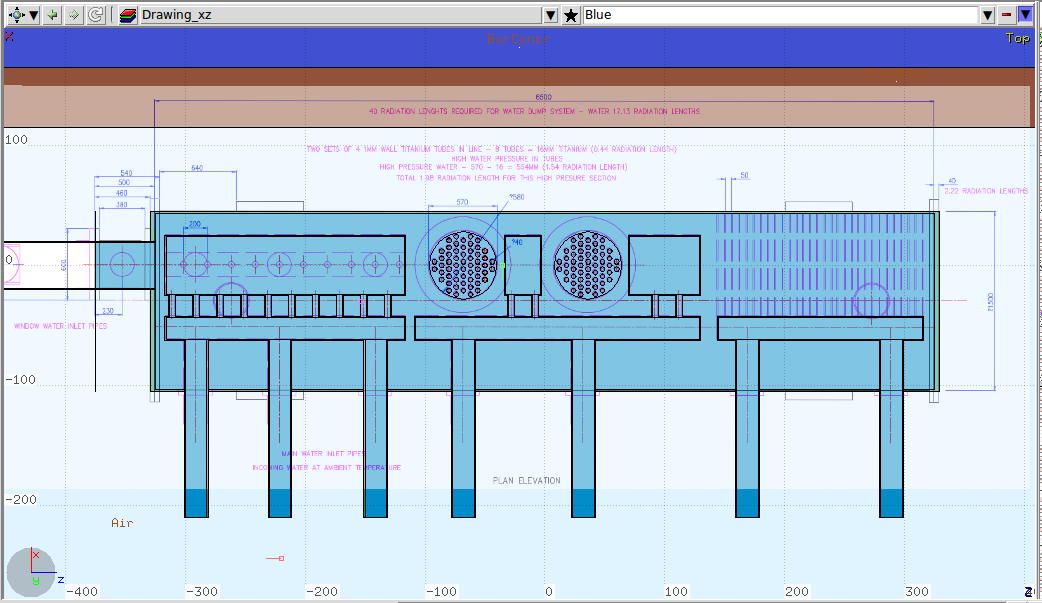
\includegraphics[width=0.5\textwidth]{Figures/BeamDump/Design2_geometry_drawing_xz.png}
\caption[Preview of the geometry construction in \flair]{Preview of the construction of the ILC beam dump using a technical drawing as a template imported into the \flair-geoviewer plug-in.}
\label{fig:BeamDumps:geoviewer}
\end{figure}

\section{ILC main beam dump designs}
\label{BeamDumps:designs}
The designs for the main beam dump in this study are based on the technical design drawings that can be found in~\cite{Smith_drawings}.
The drawings include plans for the surface building, the beam dump hall with the shielding walls around the water tank, and two different designs for the main beam dumps.
The design based on the drawing with the identification number 0-TB-0067-210-00-A~\cite{Smith_drawings} shall henceforth be called ``\designone'', the second design based on drawing 0-TB-0067-300-00-A~\cite{Smith_drawings} shall be called ``\designtwo''.
Figure~\ref{fig:BeamDumps:geometry} shows a visualization of the beam dump hall modeled within \flair. 
The innermost shielding wall around the beam dump vessel is made of iron, and has a thickness of \SI{50}{\centi\meter}.
The middle layer of shielding consists of \SI{1.5}{\meter} thick boronated concrete, surrounded by a layer of normal concrete, which has a thickness of \SI{2}{\meter}.
Boronated concrete is enriched with boron for the specific purpose of radiation shielding.
The composition of both concrete types, boronated and normal, was adapted from concrete mixtures used in Japanese research centers, as described in~\cite{concrete}. 
The infrastructure, such as cables and water pipes, is not included in the simulation geometry.
\\As mentioned in the section above, technical design drawings can be imported into \flair, and directly used as templates for the construction of the geometry.
This was done for the two beam dump designs, which will be explained in detail in the following.

\begin{figure}[hbp]
\begin{center}
\resizebox{.9\textwidth}{!}{%
\includegraphics[height=0.35\textheight]{Figures/BeamDump/Front_view_BeamDump_Tomb.png}%
\quad
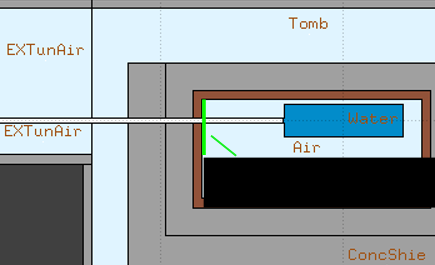
\includegraphics[height=0.35\textheight]{Figures/BeamDump/Bird_view_BeamDump_Tomb.png}%
}
\caption[Geometry visualization of the ILC main beam dump hall]{Simplified version of the beam dump hall for the purpose of visualization, containing only a simple water tank in the middle of the shielding walls. 
The geometry was modeled within \flair according to the technical drawings of the ILC beam dump facility.
The left hand picture is the front view, the beam direction is going into the page.
The right hand figure shows the top view, in which the water tank is shown in the middle of the different shielding walls. 
A \fluka specific feature is the need of having a black body void around the geometry. 
This void is the border of the tracking region, and stops all particles reaching this edge.}
\label{fig:BeamDumps:geometry}
\end{center}
\end{figure}

\subsection{\designone}
\label{BeamDumps:design:design1}
As both beam dump designs are based on a water tank system, their basic layout is very similar.
For both, the water vessel is made out of the stainless steel alloy 316L, and has a diameter of \SI{1.5}{\meter} and a length of \SI{6.5}{\meter}.
The water is pressurized to \SI{10}{\bar}.
The window between the vessel and the beam pipe has a diameter of \SI{30}{\centi\meter} and a thickness of \SI{1}{\milli\meter}.
For the window material, the titanium alloy Ti-6Al-4V is foreseen.
As can be seen from Figure~\ref{fig:BeamDumps:design1}, the vessel contains several pipes belonging to an inner vortex system.
The turbulence of the water allows the arising heat of up to \SI{150}{\celsius} from the beam power to dissipate~\cite[p. 3]{Dump_report}.
\\Overall, the water volume represents a material budget of 18 radiation lengths (\si{\xzero}), which yields an attenuation of about \SI{33}{\percent}.
An additional \SI{9}{\xzero} are placed in the end of the vessel in the form of water cooled copper plates~\cite[p. 2]{Dump_report}.

\begin{figure}[h]
 \centering
  \begin{subfigure}[b]{0.49\textwidth}
   \centering
    \includegraphics[width=\textwidth]{Figures/BeamDump/TB-0067-210-00-A_yz_view.png}
   \caption{Technical drawing, yz-view}
   \end{subfigure}
   \hfill
    \begin{subfigure}[b]{0.49\textwidth}
   \centering
    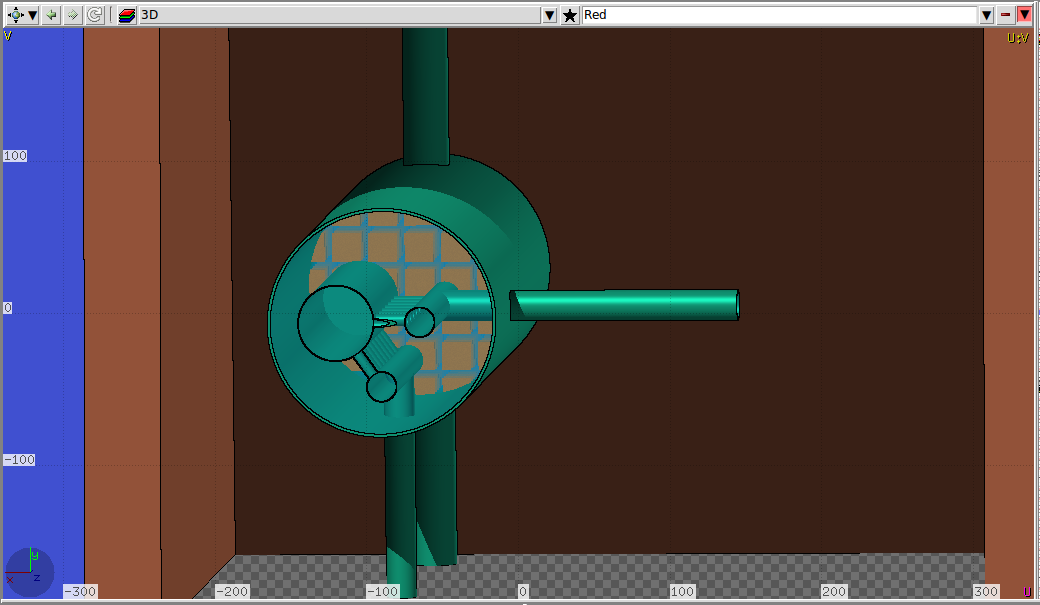
\includegraphics[width=\textwidth]{Figures/BeamDump/Design1_geometry_3Dinside.png}
   \caption{\fluka model, 3D-view}
   \end{subfigure}
   \caption[ILC main beam dump design 1]{Figure (a) shows the yz-view of the beam dump \designone from the technical drawing.
   The \fluka model constructed within \flair is shown in Figure (b).}
   \label{fig:BeamDumps:design1}
 \end{figure}

\subsection{\designtwo}
\label{BeamDumps:design:design2}
The basic layout explained above for \designone was also adopted for \designtwo, so that the measurements of the vessel and the window are the same for both designs.
The main difference is the addition of a high pressure water section in the middle of the vessel  for \designtwo.
Figure~\ref{fig:BeamDumps:design2} shows the 3D model of \designtwo implemented within \flair, with the high pressure water section in the middle. 
The titanium tubes of this system have a diameter of \SI{4}{\centi\meter}, through which high pressure water is pumped.
\\The vortex system shows also a different design approach.
More tubes connect the vortex system with the outside pumps.
The copper plates in this design are placed in the end of the vessel as well, for an additional \SI{9}{\xzero}.

\begin{figure}[h]
 \centering
  \begin{subfigure}[b]{0.49\textwidth}
   \centering
    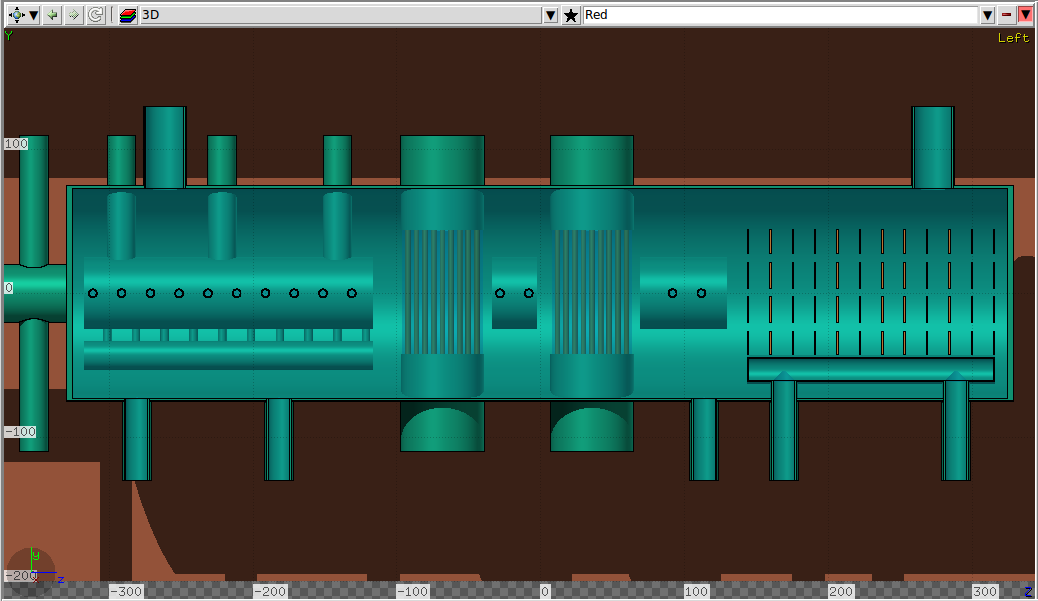
\includegraphics[width=\textwidth]{Figures/BeamDump/Design2_geometry_3Dinside3.png}
   \caption{\fluka model, yz-view}
   \end{subfigure}
   \hfill
    \begin{subfigure}[b]{0.49\textwidth}
   \centering
    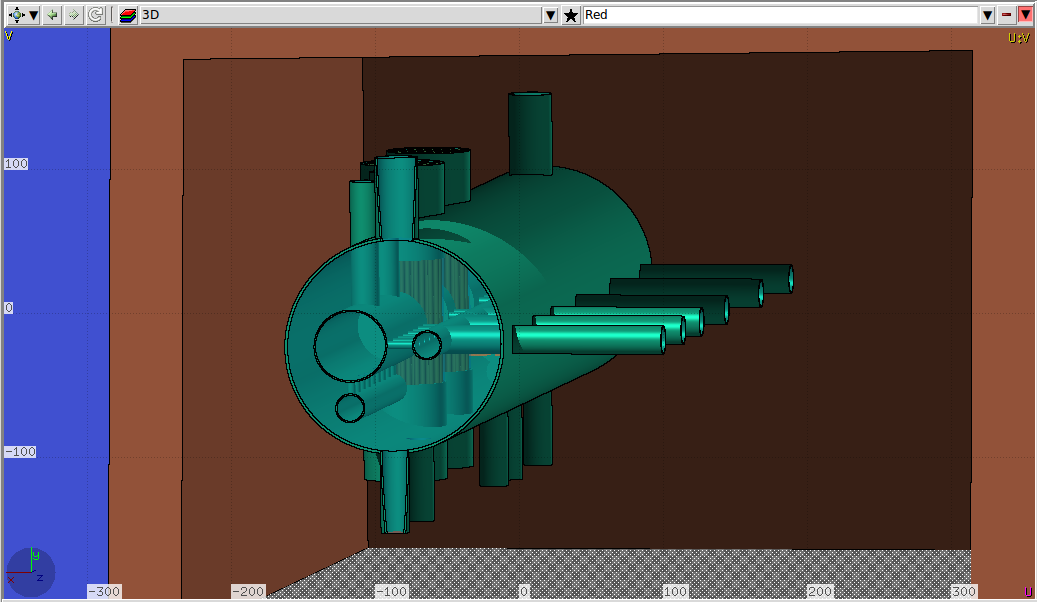
\includegraphics[width=\textwidth]{Figures/BeamDump/Design2_geometry_3Dinside1.png}
   \caption{\fluka model, 3D-view}
   \end{subfigure}
   \caption[ILC main beam dump design 2]{Figure (a) shows the yz-view of the \fluka model of the beam dump \designtwo, the 3D-view is shown in Figure (b).}
   \label{fig:BeamDumps:design2}
 \end{figure}

\section{Simulation studies of the beam dump surrounding}
\label{BeamDumps:sim_surrounding}
For the \fluka simulation of the ILC beam being dumped into the water tanks of \designone and \designtwo as explained above, the running scheme of the ILC1000B~\cite[p. 11]{TDR1} stage was chosen.
The beam bunches, which are considered un-collided and un-disrupted for this simulation study, have a bunch population of \num{1.74e10} electrons, and a beam energy of \SI{500}{\GeV}.
One beam pulse has \num{2450} bunches and a duration of \SI{896.7}{\micro\second}.
At the location of the main beam dump, the bunches have a size of $\sigma_x = $\,\SI{2.4}{\milli\meter} and $\sigma_y = $\,\SI{0.22}{\milli\meter}.
\\In the \fluka model, the origin of the coordinate system is set to the center axis of the beam pipe in x and y, and to the middle of the water vessel in z.
The beam bunches therefore start at a negative z-position of \SI{-10}{\meter} along the beam pipe center axis.
This becomes clear in Figure~\ref{fig:BeamDumps:Energy}, which shows the first \fluka result, the deposited energy per bunch.
The following sections present the expected dose rate and the particle densities.

\subsection{Energy deposition}
\label{BeamDumps:sim_surrounding:Energy}
In \fluka, various physics quantities can be measured as spatial densities or as double differential distributions in so-called scoring cards.
The measured data can then be plotted with \flair.
\\In this subsection, the energy deposition per volume is presented in the beam dump surroundings.
Figures~\ref{fig:BeamDumps:Energy} (a) and (b) show the results in the xz-plane of the geometry for y = 0 $\pm$ \SI{3}{\centi\meter}.
For two dimensional plots, the outlines of the geometry model can be superimposed in the correct plane.
In this way, the spatial distribution of the measured physics quantity can directly be associated with the material allocation of the geometry.
The comparison between Figure (a) and (b) shows that the energy deposited in \designone is well contained within the iron shielding wall.
Closest to the vessel, energies of up to about \SI{e6}{\GeV\per\centi\meter\cubed} are deposited in the iron.
For \designtwo however, the spread in the energy deposition reaches beyond the first shielding walls.
The reason for this is the larger material density in \designtwo in the form of the high pressure water section in the middle of the vessel, which leads to enhanced particle showering.
\\Figures~\ref{fig:BeamDumps:Energy} (c) and (d) show the maximum values of every bin in Figures (a) and (b).
The overall distribution of the deposited energy over z is smooth, with a maximum shortly before the vessel center.
Nevertheless, the distribution has several sharp peaks which can be identified at locations with large material density.
For \designone, the first sharp peak at z\,$\approx$\,\SI{-230}{\centi\meter} corresponds to the front side of the vortex tube, the back side of the same tube is also visible through the second peak at z\,$\approx$\,\SI{110}{\centi\meter}.
The third peak at z\,$\approx$\,\SI{220}{\centi\meter} is caused by the beam hitting the first copper plates in the end of the vessel.
\\Accordingly, the sharp peaks in Figure~\ref{fig:BeamDumps:Energy} (d) for \designtwo also correspond to locations with a higher material density.
The first two peaks at z\,$\approx$\,\SI{-100}{\centi\meter} and z\,$\approx$\,0 represent the high water pressure sections with their titanium tubes.
The last peak at z\,$\approx$\,\SI{120}{\centi\meter} originates from the first copper plates, which in this design are located closer to the vessel center.
The absolute value for the maximum energy deposited per bunch is between $\sim$\SI{1.4e8}{\GeV\per\centi\meter\cubed} and \SI{1.1e9}{\GeV\per\centi\meter\cubed}, for \designone and \designtwo respectively.
\begin{figure}[!t]
 \centering
  \begin{subfigure}[b]{0.49\textwidth}
   \centering
    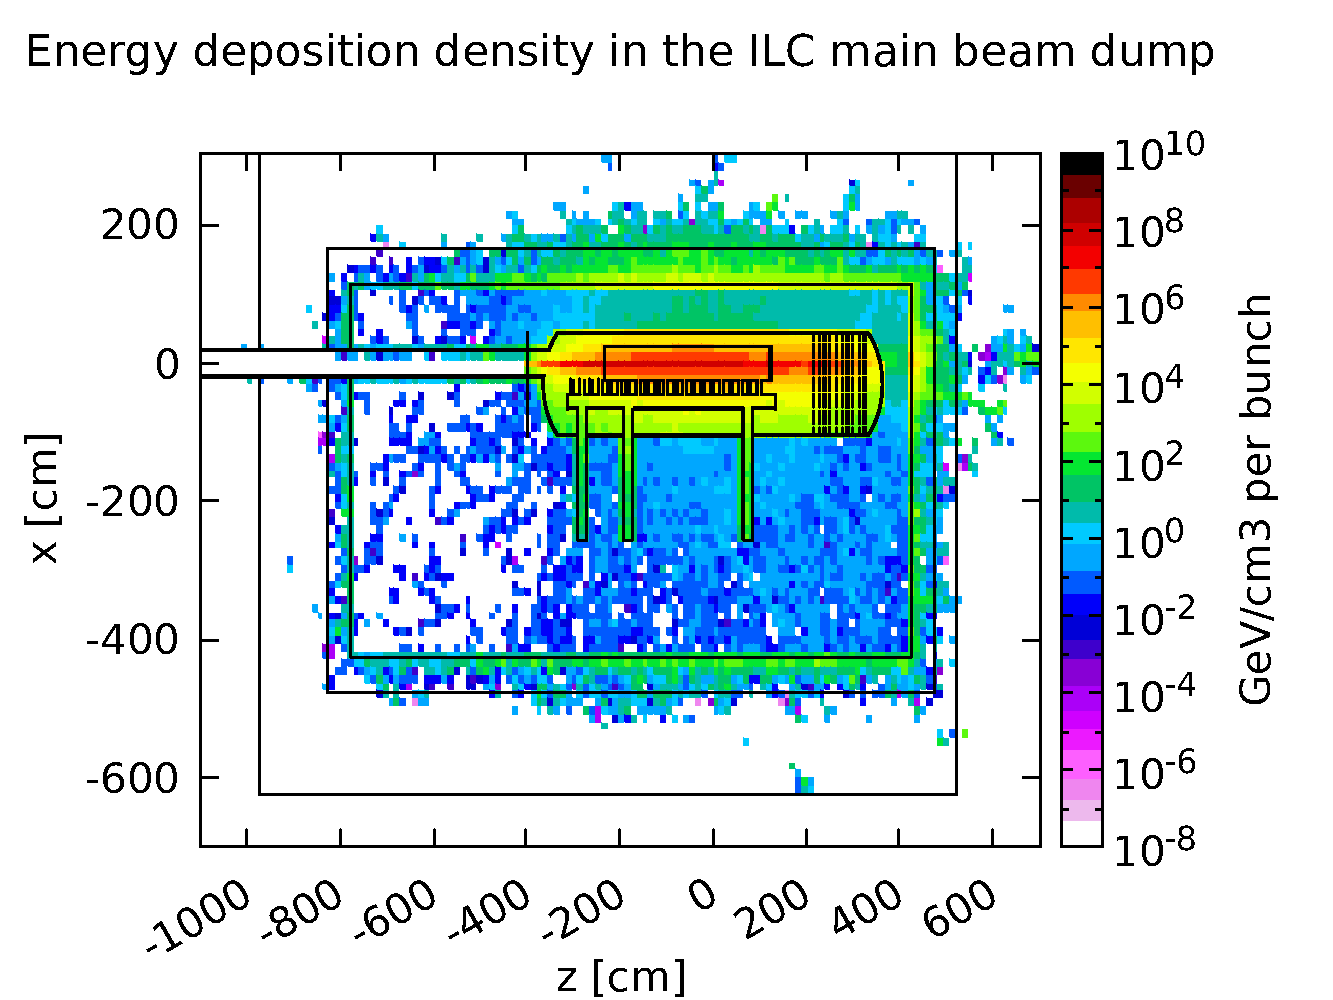
\includegraphics[width=\textwidth]{Figures/BeamDump/Energy_deposition_xz_Design1.pdf}
   \caption{\designone, xz-plane}
   \end{subfigure}
   \hfill
    \begin{subfigure}[b]{0.49\textwidth}
   \centering
    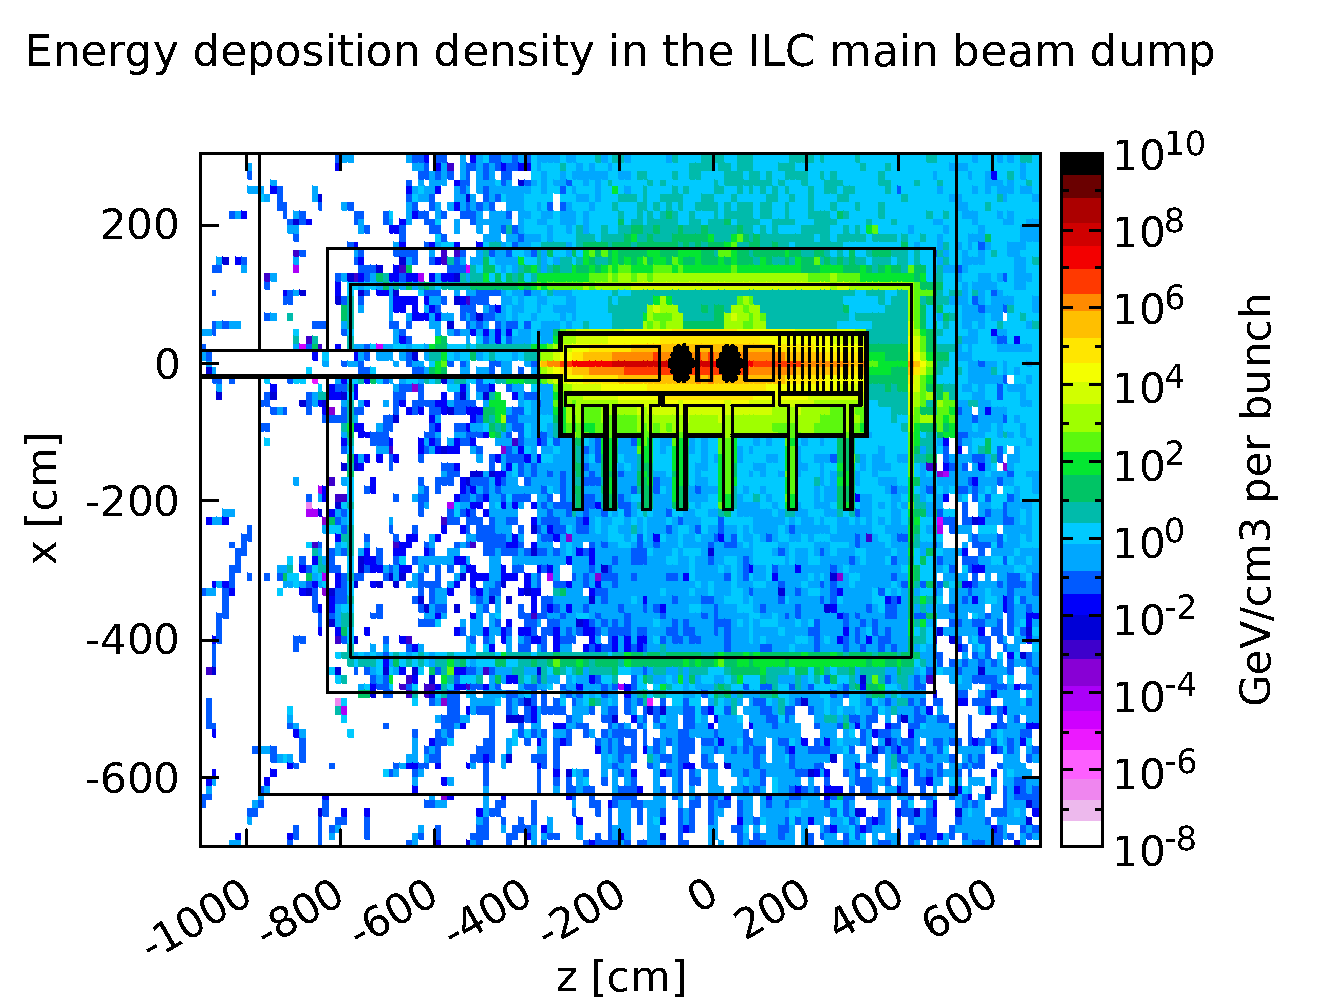
\includegraphics[width=\textwidth]{Figures/BeamDump/Energy_deposition_xz_Design2.pdf}
   \caption{\designtwo, xz-plane}
   \end{subfigure}\\ \vspace*{0.3cm}
     \begin{subfigure}[b]{0.485\textwidth}
   \centering
    \includegraphics[height=0.245\textheight]{Figures/BeamDump/Energy_deposition_1DMax_z_Design1_2.png}
   \caption{\designone, z-projection}
   \end{subfigure}
   \hfill
    \begin{subfigure}[b]{0.485\textwidth}
   \centering
    \includegraphics[height=0.248\textheight]{Figures/BeamDump/Energy_deposition_1DMax_z_Design2.png}
   \caption{\designtwo, z-projection}
   \end{subfigure}
   \caption[Energy deposition in the ILC main beam dump]{\fluka result of the energy deposition density of one beam bunch in the ILC beam dump \designone (a) and \designtwo (b).
   The view is in the xz-plane of the beam dump surroundings including the shielding walls.
   The color scale shows the deposited energy in \si[detect-all]{\GeV}/\si{\centi\meter\cubed} per bunch.
   \\Figures (c) and (d) show the maximum values of the energy deposition as a projection on the z axis.}
   \label{fig:BeamDumps:Energy}
\end{figure}
 
\subsection{Irradiation dose}
\label{BeamDumps:sim_surrounding:Dose} 
From the deposited energy, \fluka can calculate the instantaneous dose equivalent of the beam dumps and their surroundings.
Figure~\ref{fig:BeamDumps:Dose} (a) and (b) show the \fluka results of the spatial distribution of the dose from one bunch in the xz-plane, (c) and (d) show the projection of the maximum values onto the z axis, equivalent to the energy deposition plots before.
\\The distributions are comparable for both beam dump designs, the projection plots also again show sharp peaks at the locations of high material density.
The maximum dose equivalent from one bunch reaches about \SI{82}{\sievert} in \designone and \SI{105}{\sievert} in \designtwo.
\begin{figure}[!h]
 \centering
  \begin{subfigure}[b]{0.49\textwidth}
   \centering
    \includegraphics[width=\textwidth]{Figures/BeamDump/Dose_equivalent_total_Design1.pdf}
   \caption{\designone, xz-plane}
   \end{subfigure}
   \hfill
    \begin{subfigure}[b]{0.49\textwidth}
   \centering
    \includegraphics[width=\textwidth]{Figures/BeamDump/Dose_equivalent_total_Design2.png}
   \caption{\designtwo, xz-plane}
   \end{subfigure}\\ \vspace*{0.3cm}
     \begin{subfigure}[b]{0.485\textwidth}
   \centering
    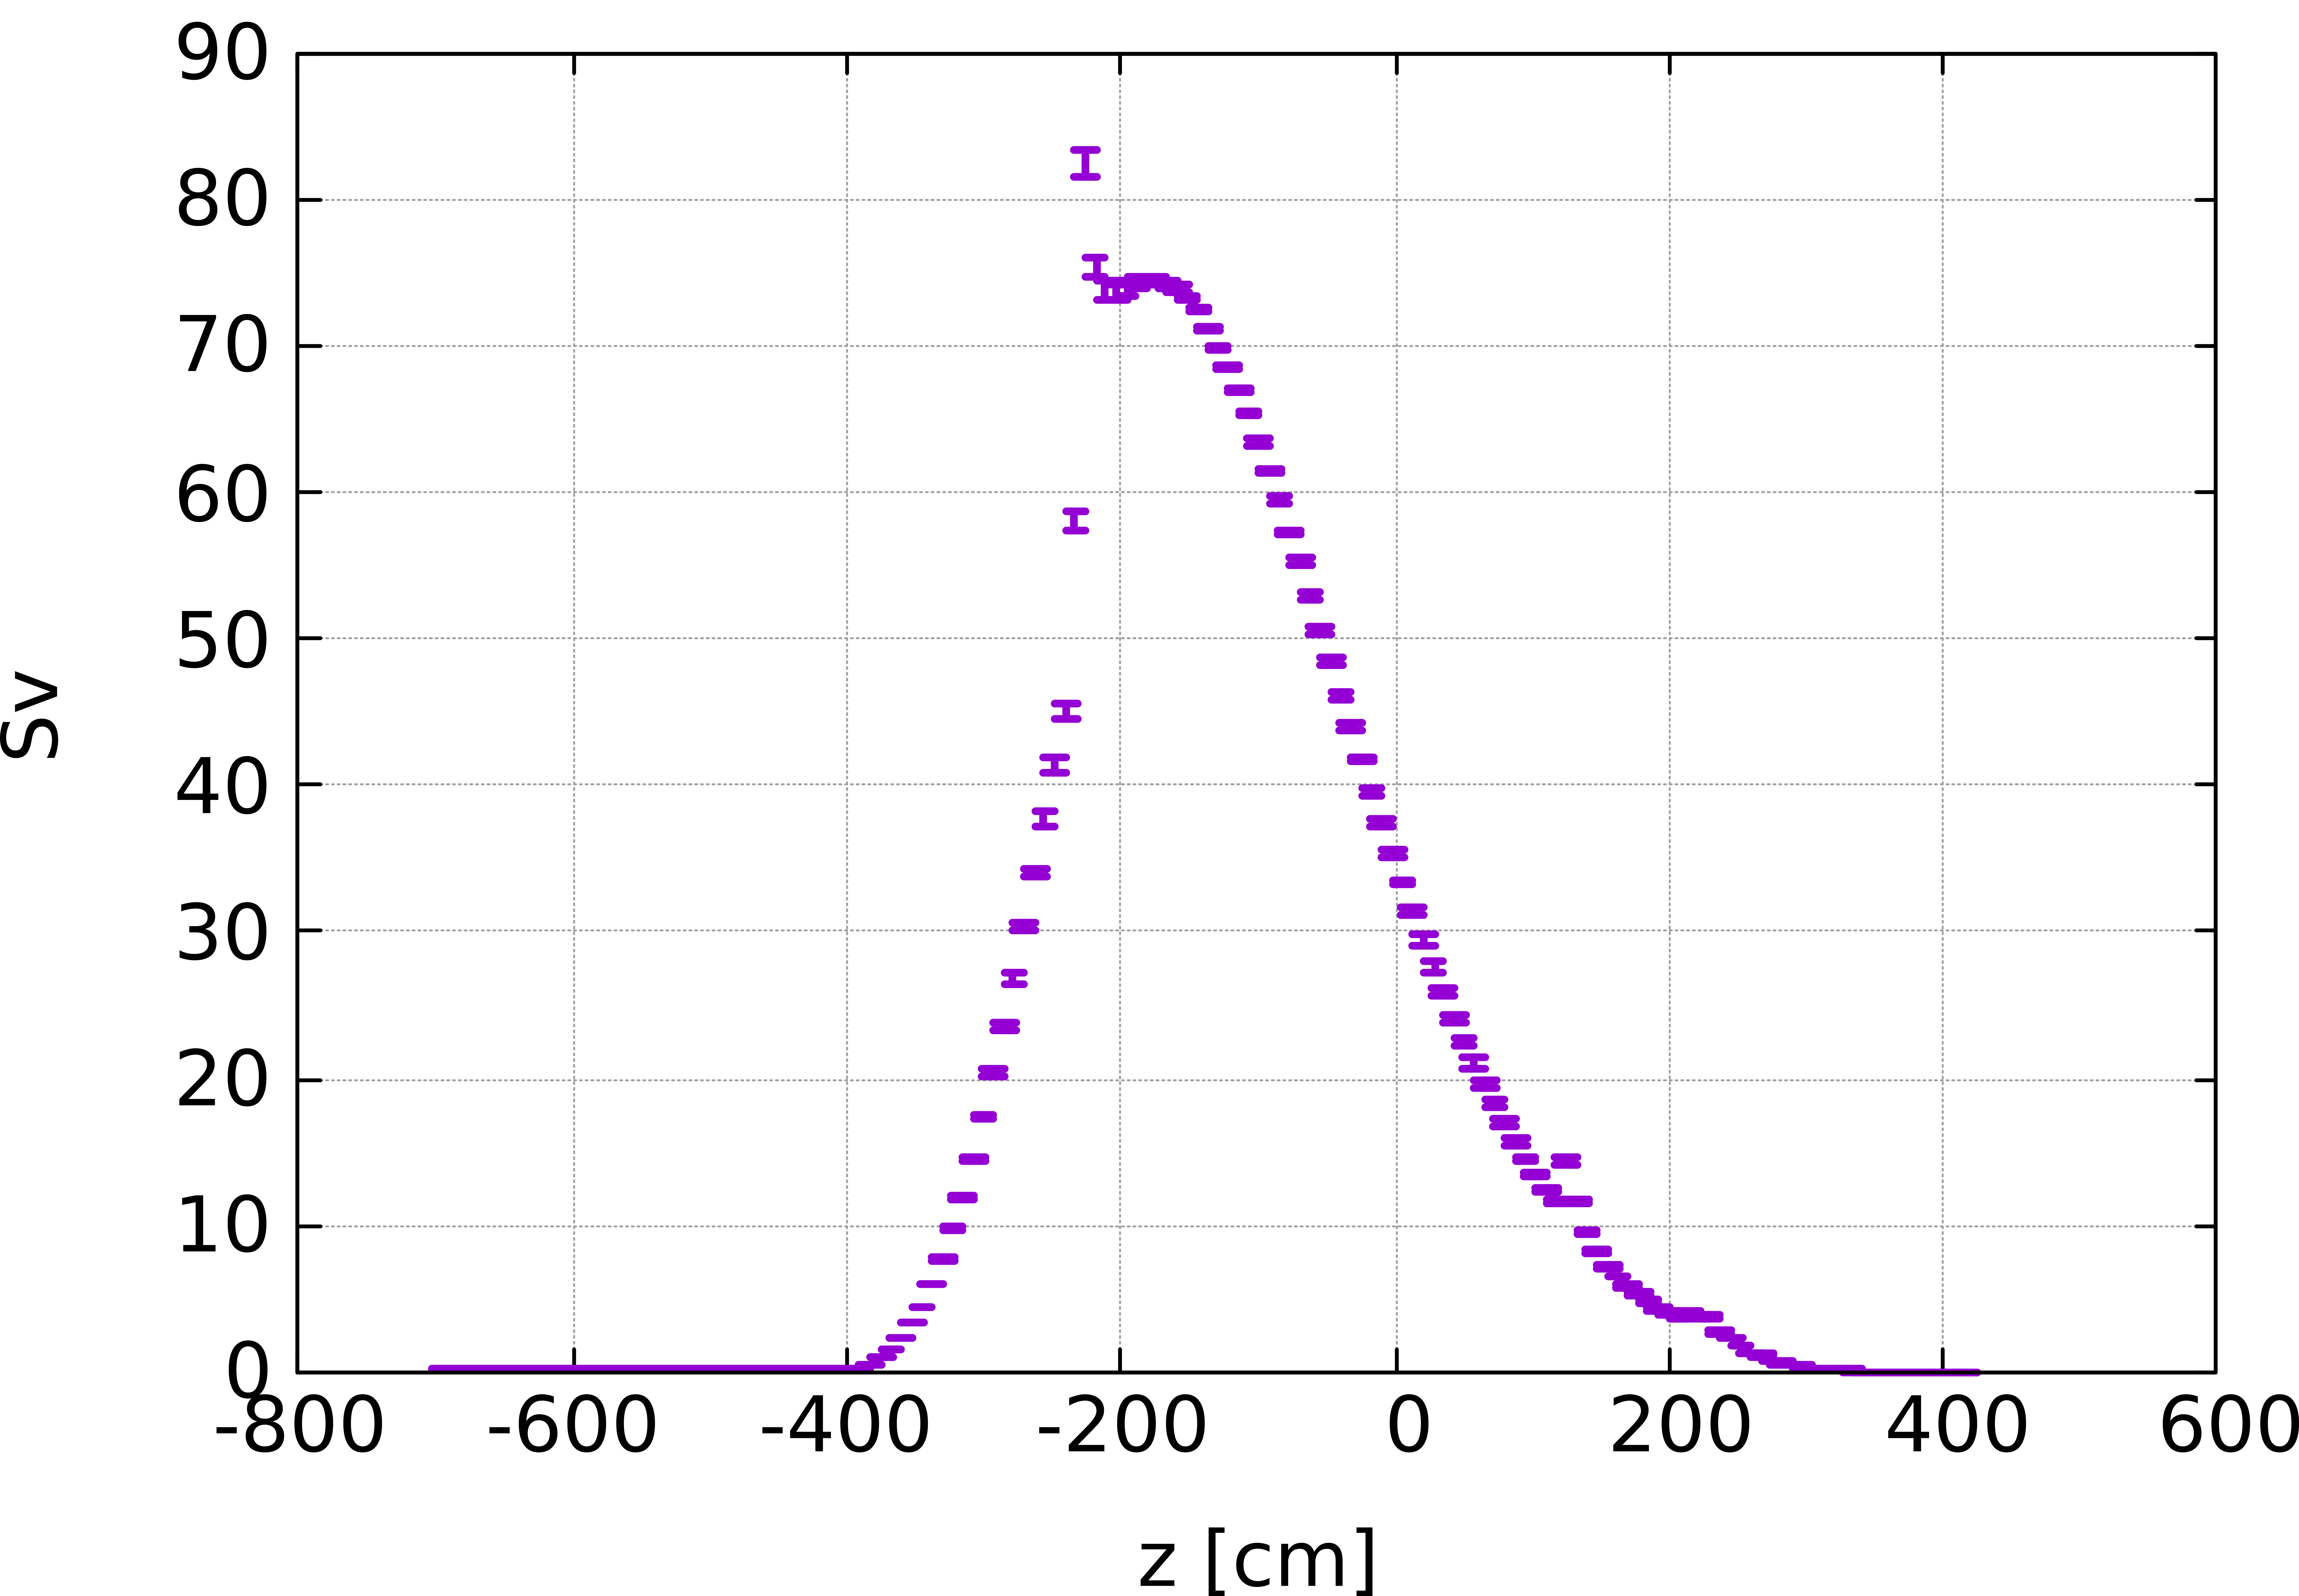
\includegraphics[height=0.24\textheight]{Figures/BeamDump/Dose_equivalent_total_1DMax_z_Design1.png}
   \caption{\designone, z-projection}
   \end{subfigure}
   \hfill
    \begin{subfigure}[b]{0.485\textwidth}
   \centering
    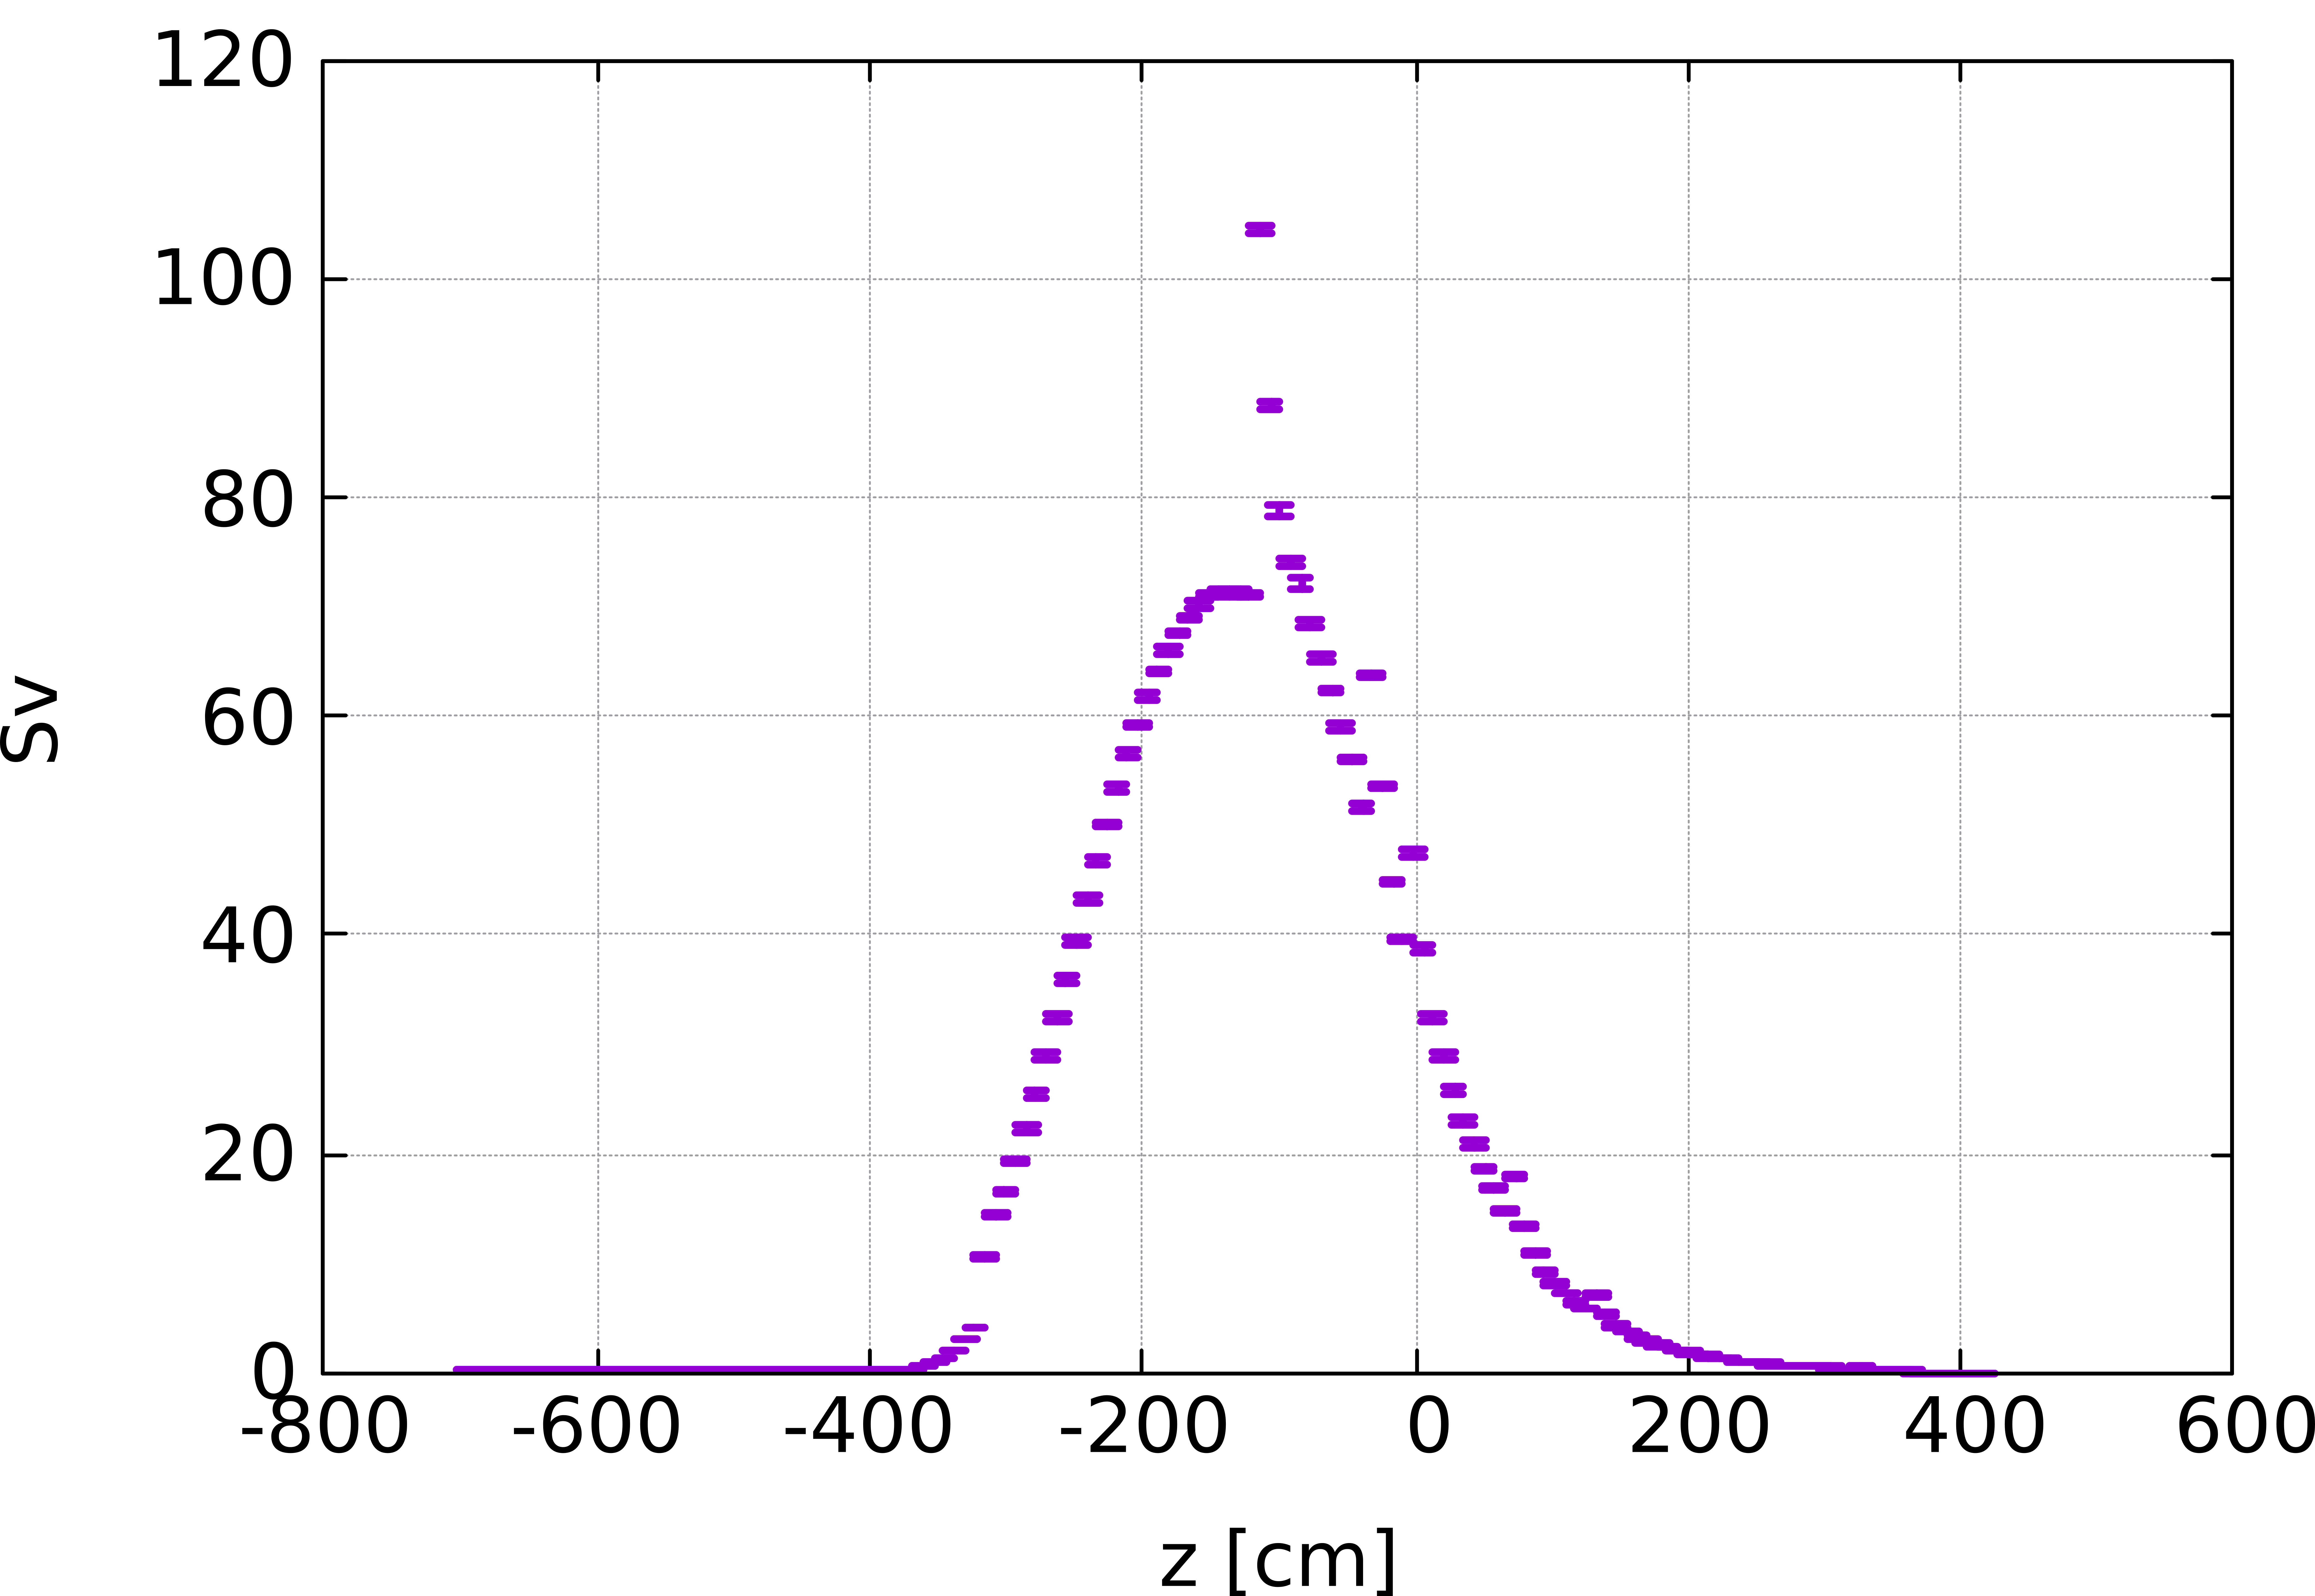
\includegraphics[height=0.24\textheight]{Figures/BeamDump/Dose_equivalent_total_1DMax_z_Design2.png}
   \caption{\designtwo, z-projection}
   \end{subfigure}
   \caption[Dose equivalent in the ILC main beam dump]{\fluka result of the dose equivalent from one beam bunch in the ILC beam dump \designone (a) and \designtwo (b) and their surroundings.
   The view is in the xz-plane of the beam dump surroundings including the shielding walls.
   The color scale shows the dose in \si[detect-all]{\milli\sievert} per bunch.
   \\Figures (c) and (d) show the maximum values of the dose as a projection on the z axis.
   The dose equivalent is here given in \si[detect-all]{\sievert}.}
   \label{fig:BeamDumps:Dose}
\end{figure}
\FloatBarrier
From this, the remaining dose rate can be calculated after certain cooling times.
It was assumed that there has been full beam operation for one month, after which the accelerator is turned off.
Considering the cooling times of one minute, one hour, one day, one month, and one year after the moment of the beam operation stop, the remaining dose rate decreases over time.
Figure~\ref{fig:BeamDumps:DoseRate} in the Appendix shows the spatial distribution of the dose rate for \designone and \designtwo for the cooling times mentioned above.
The comparison of the dose rate as a function of the cooling time for the two designs is then given in Figure~\ref{fig:BeamDumps:DoseRate_Comparison}.
\begin{figure}[!h]
\centering
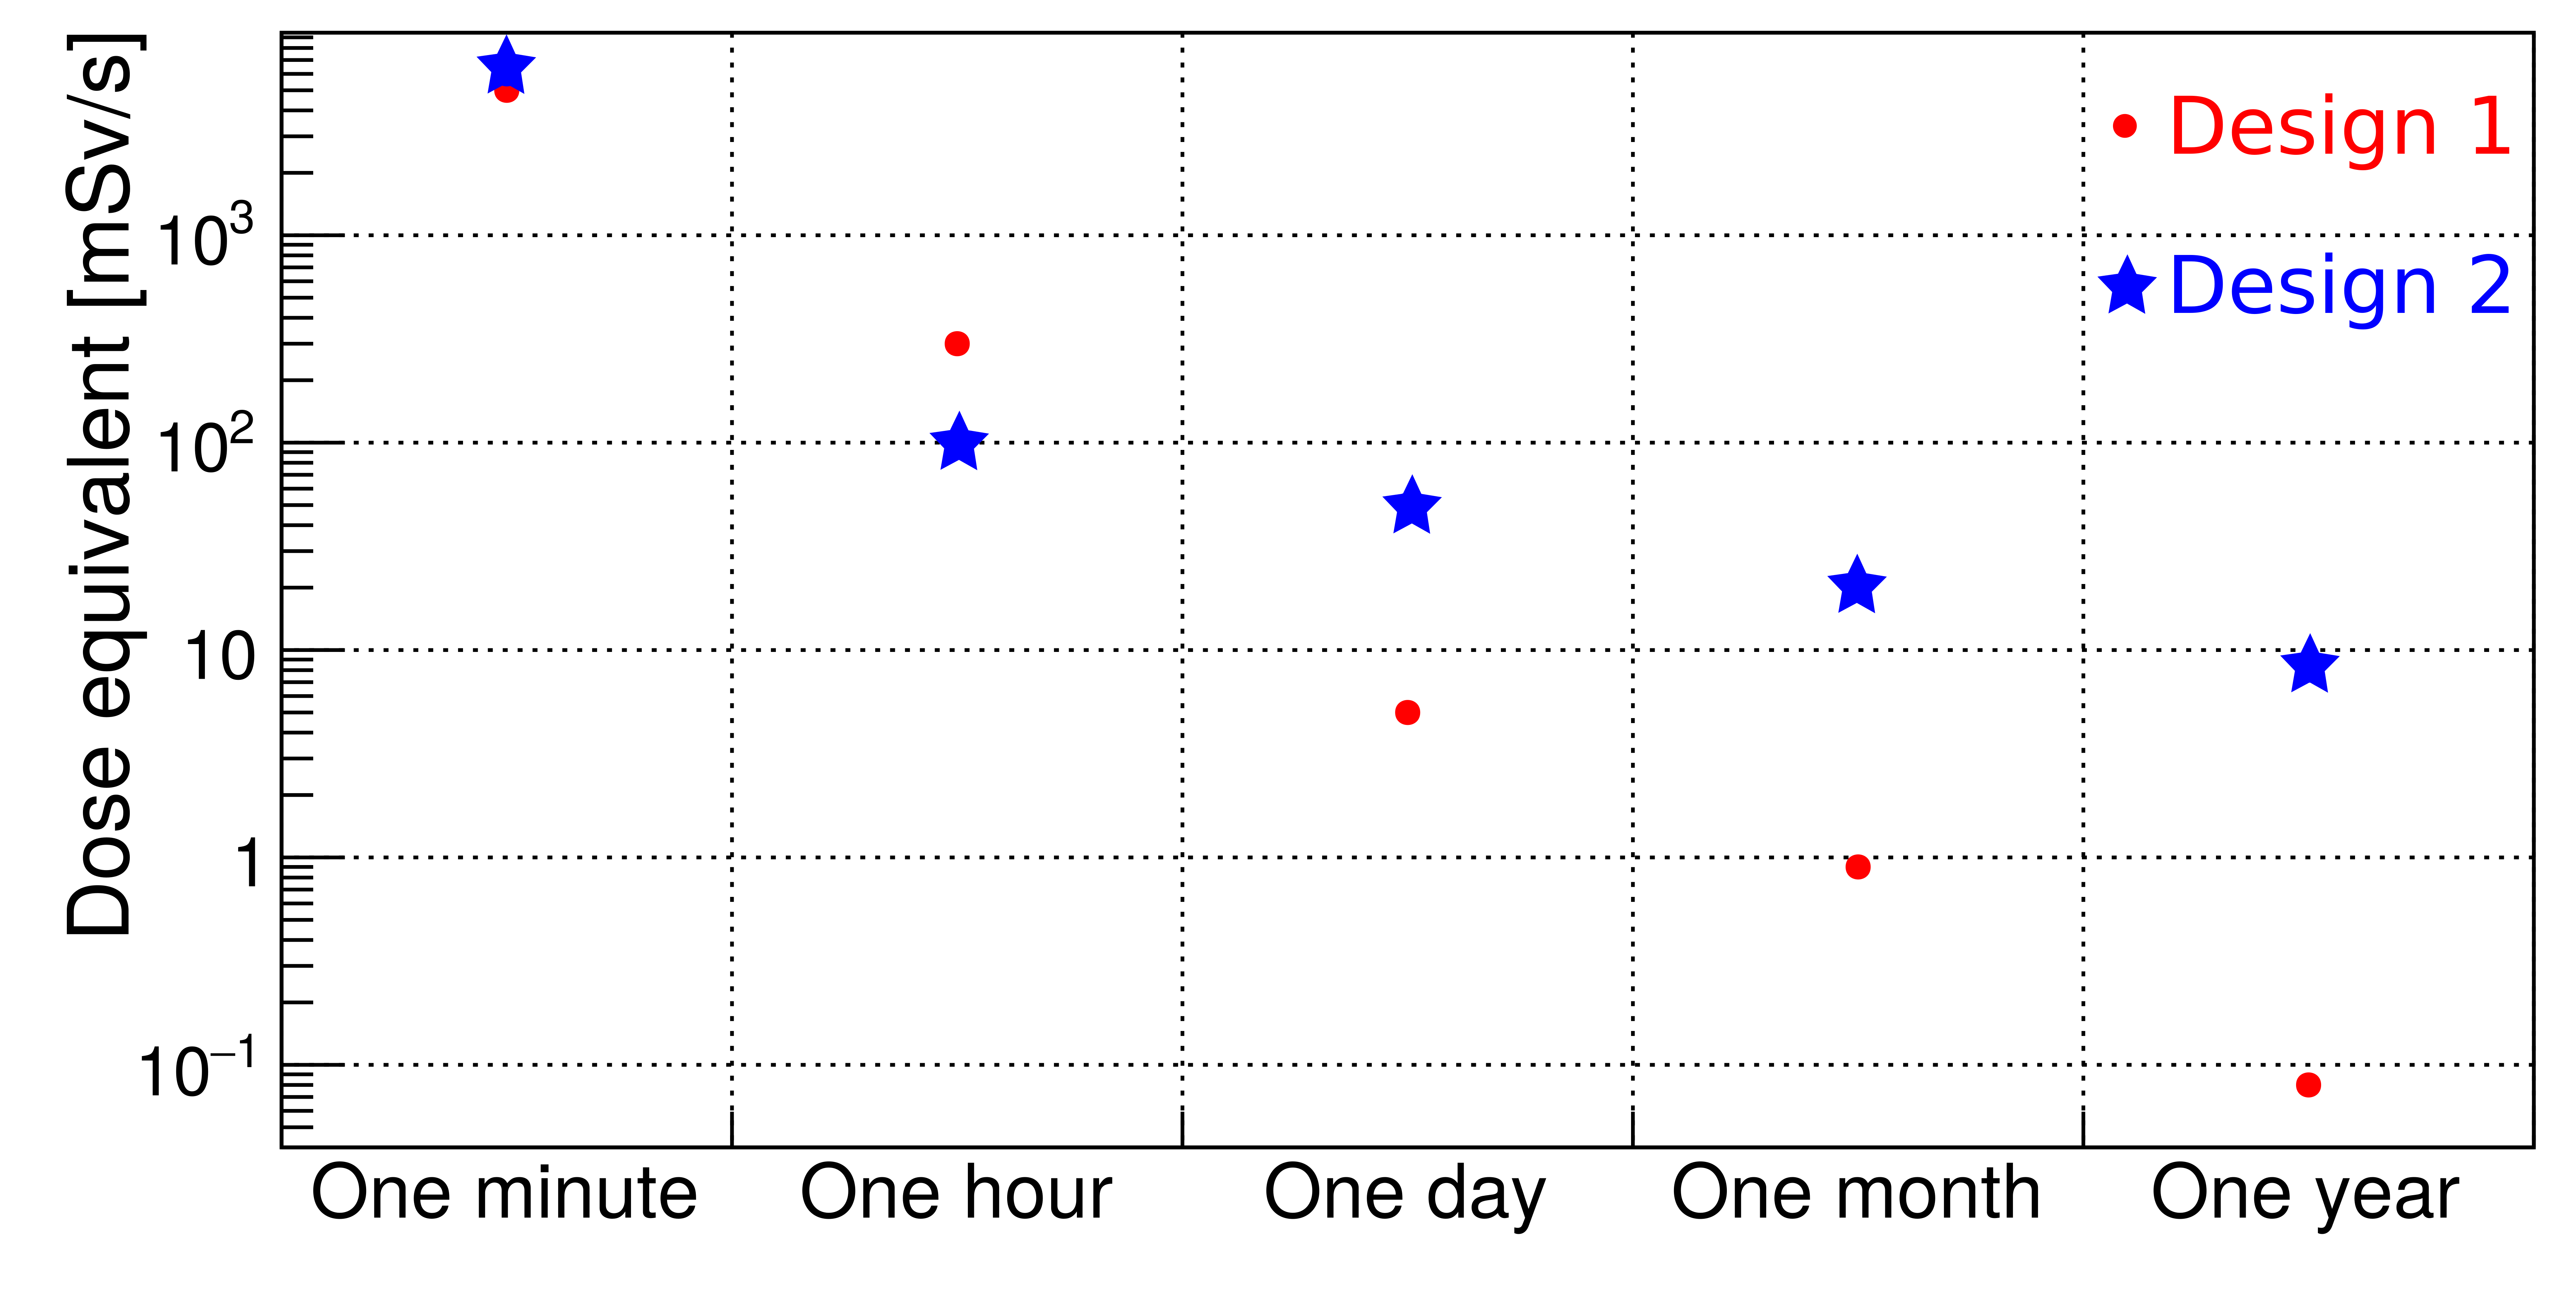
\includegraphics[width=0.65\textwidth]{Figures/BeamDump/DoseEQ_Time_Comparison.png}
\caption[Dose rate comparison of the ILC main beam dump designs]{Comparison of the maximum dose rate over the cooling time for the two ILC main beam dump designs \designone and \designtwo.}
\label{fig:BeamDumps:DoseRate_Comparison}
\end{figure}
\begin{figure}[!h]
 \centering
    \begin{subfigure}[b]{0.49\textwidth}
   \centering
    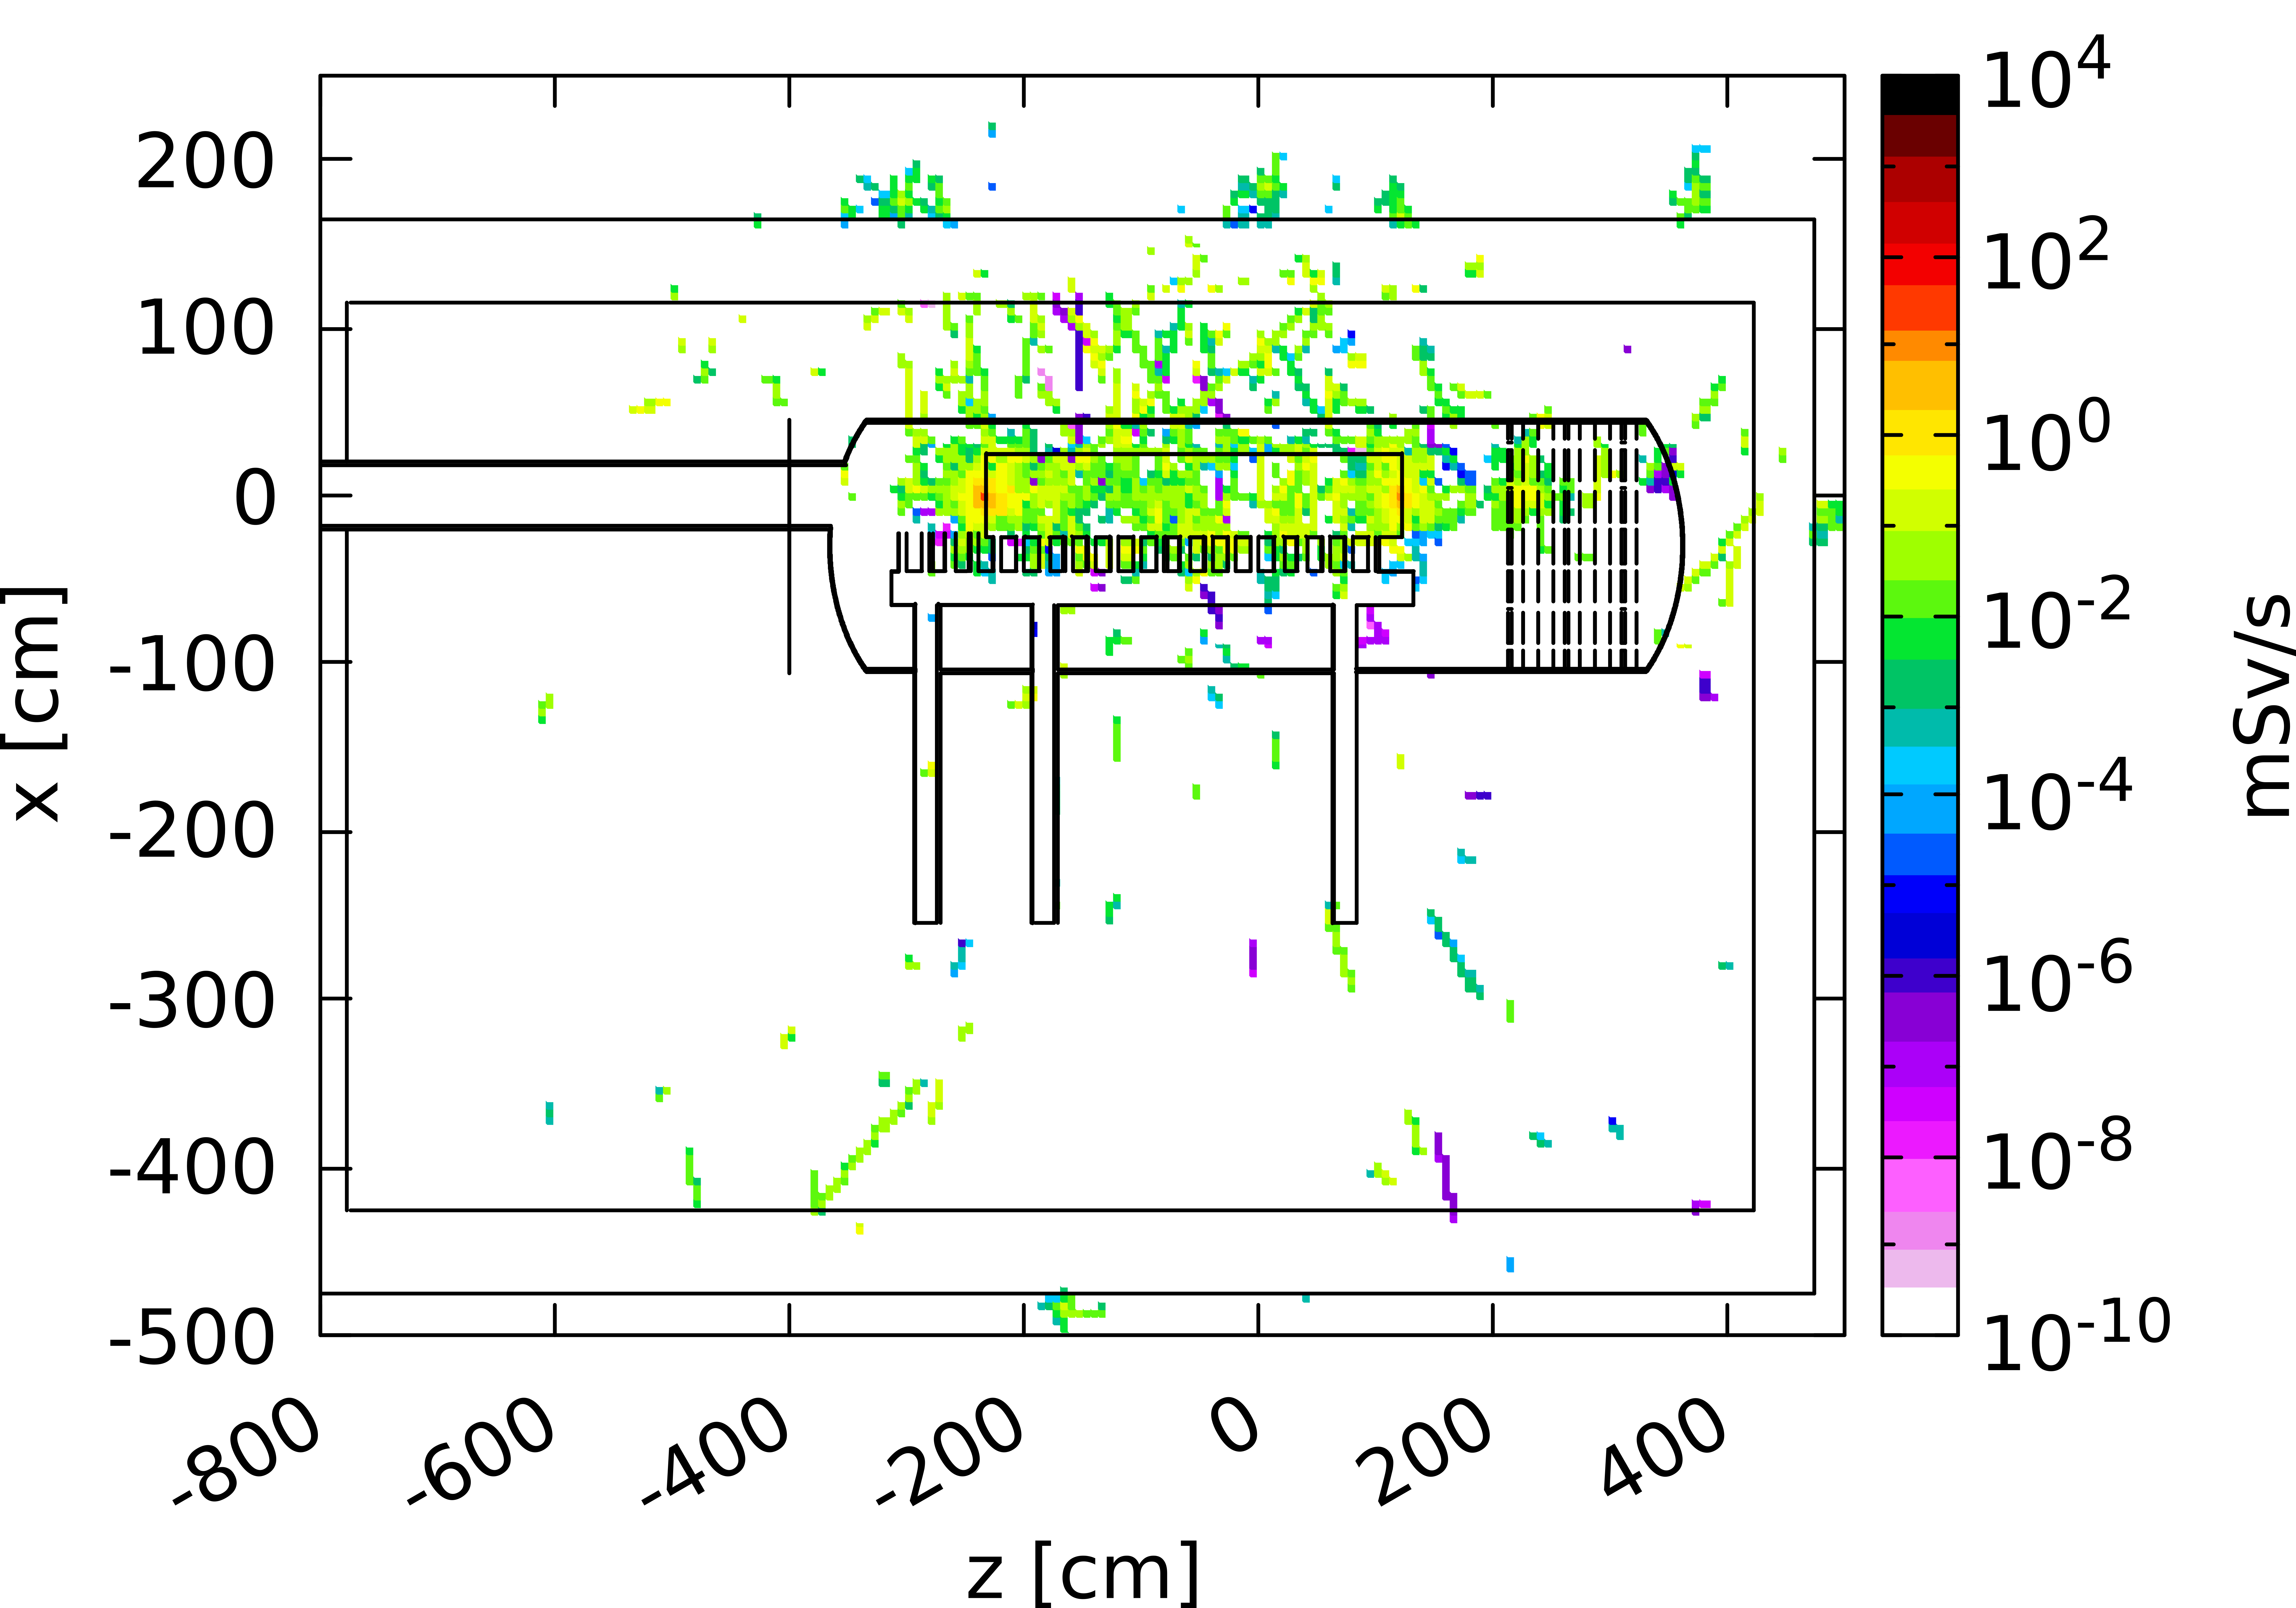
\includegraphics[width=\textwidth]{Figures/BeamDump/Design1_5.png}
   \caption{\designone, 1 year}
   \end{subfigure} 
   \hfill
    \begin{subfigure}[b]{0.49\textwidth}
   \centering
    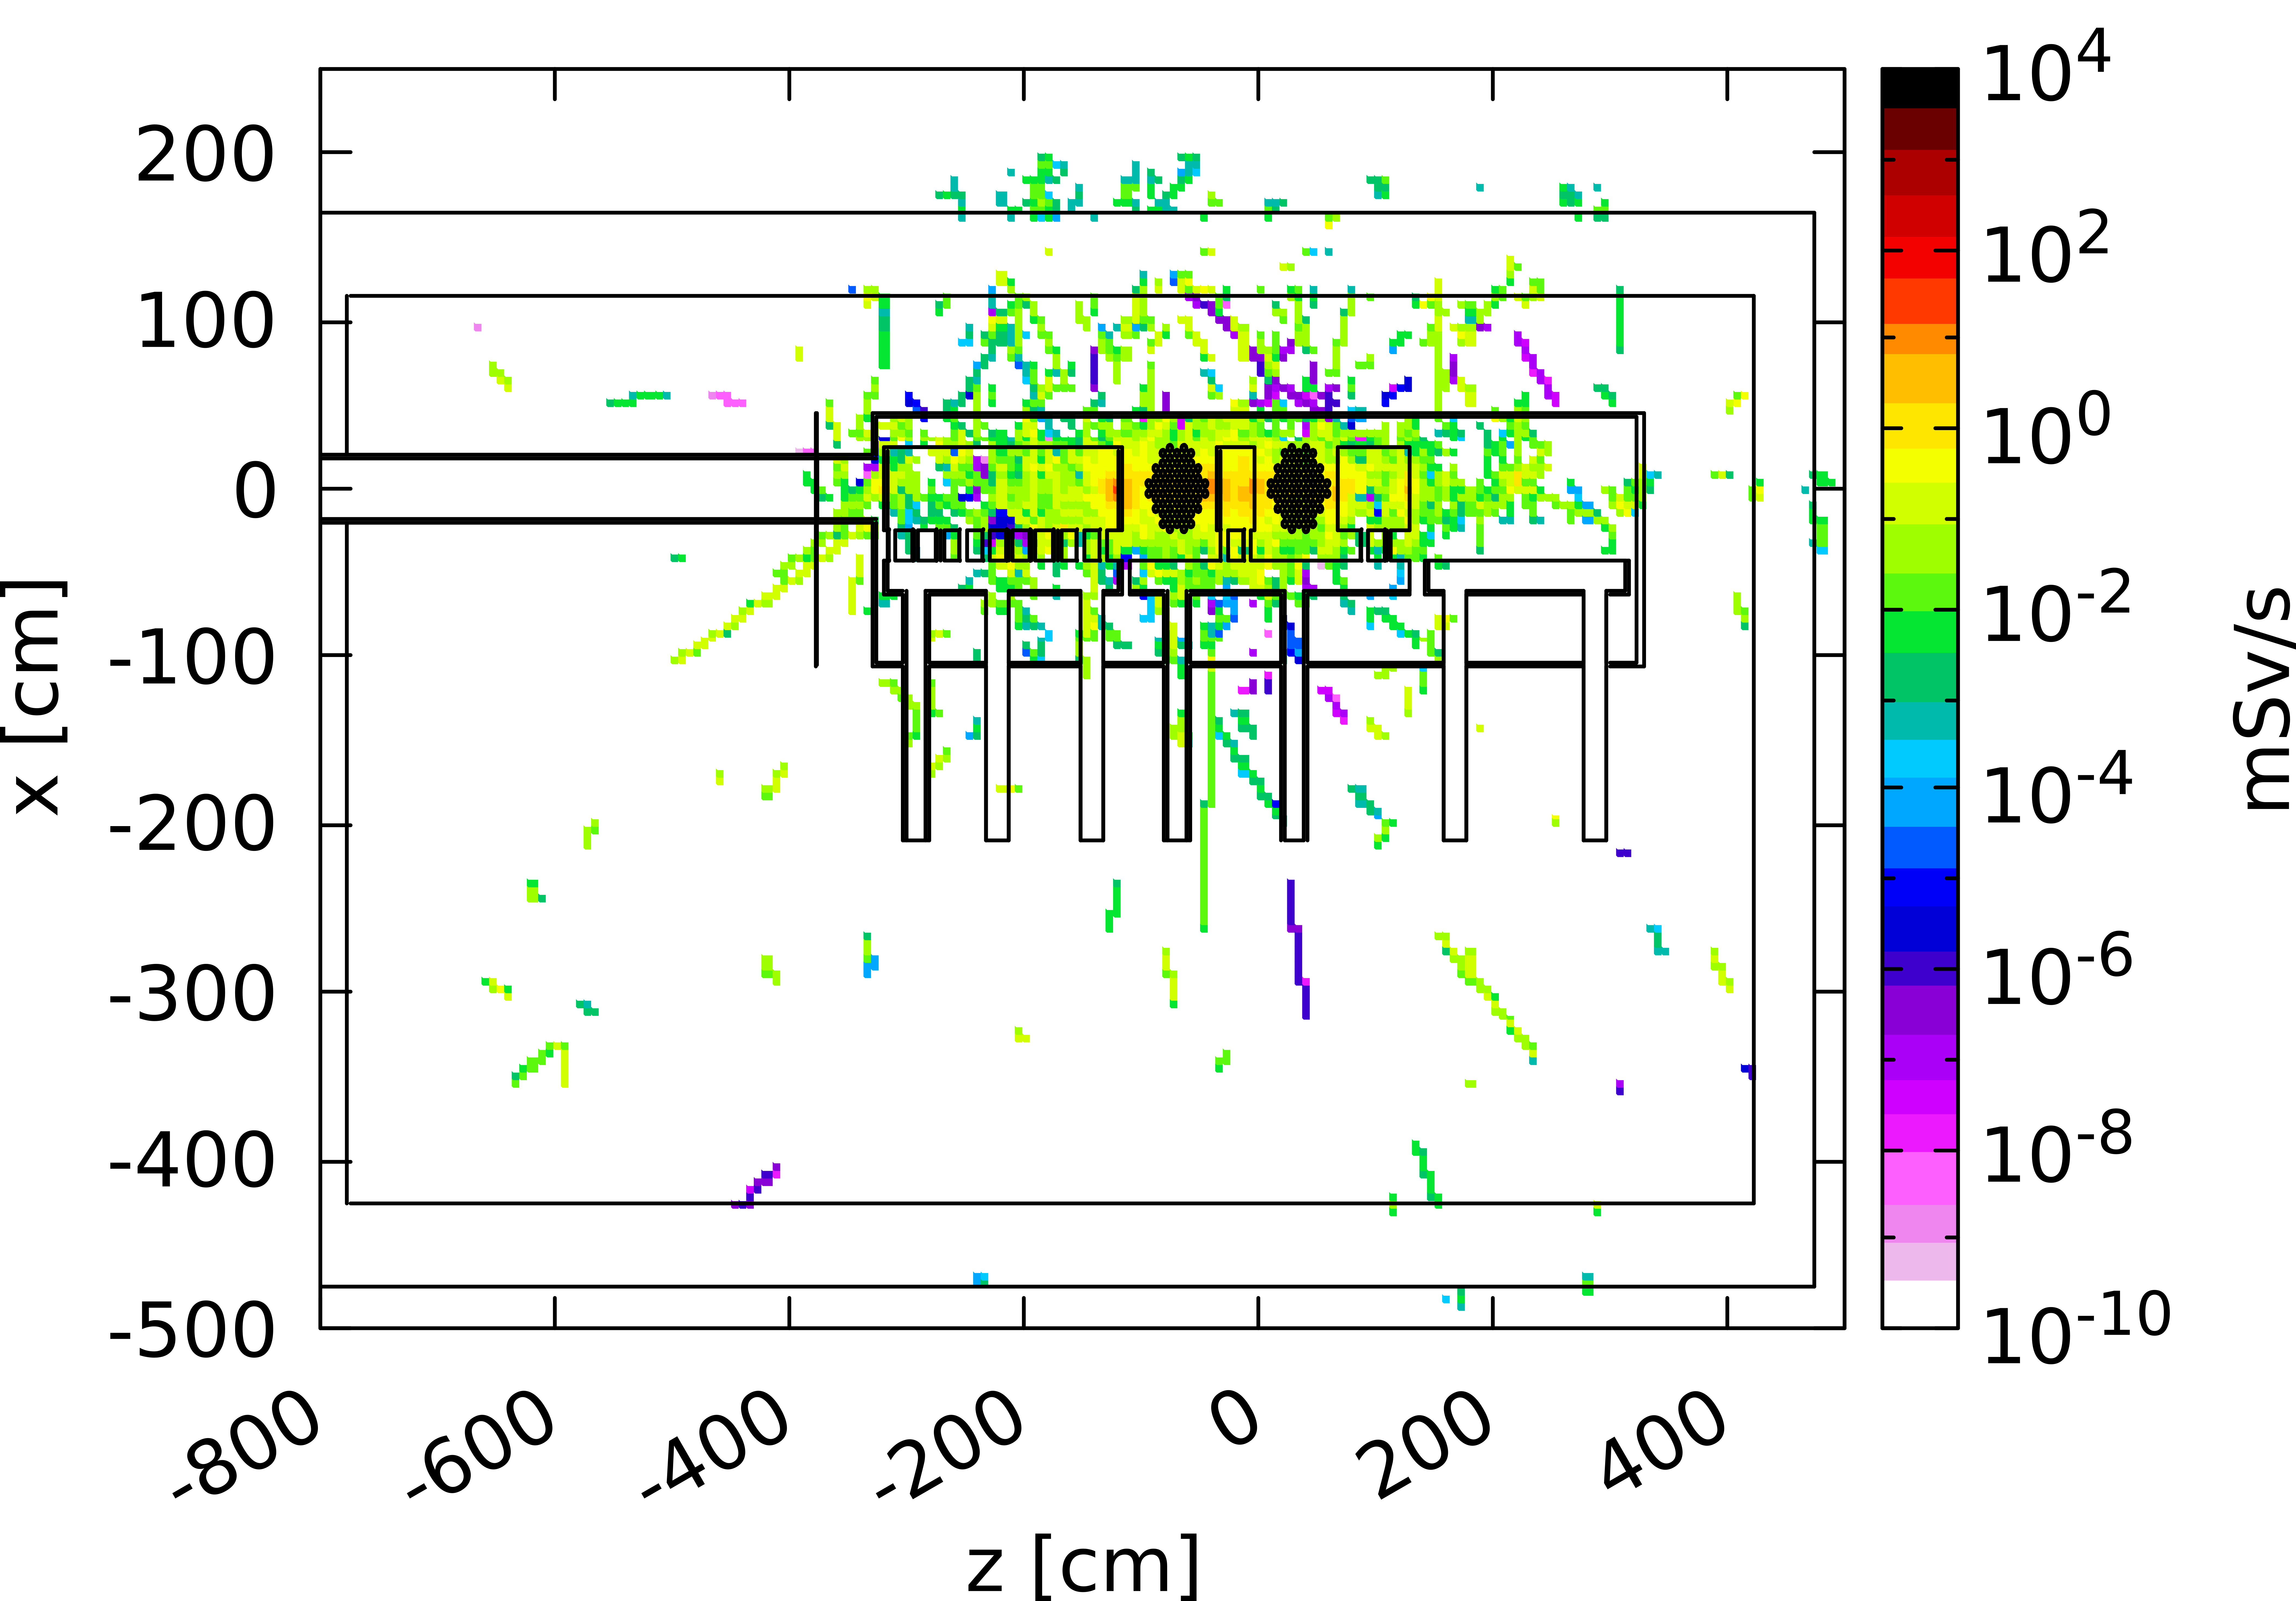
\includegraphics[width=\textwidth]{Figures/BeamDump/Design2_5.png}
   \caption{\designtwo, 1 year}
   \end{subfigure}
   \caption[Dose rate in the ILC main beam dump after one year]{\fluka result of the dose rate in the ILC beam dump \designone (a) and \designtwo (b) and their surrounding after one month of beam operation and one year of cooling time.
   The view is in the xz-plane of the beam dump surrounding including the shielding walls.
   The color scale shows the dose rate in \si{\milli\sievert\per\second}.}
   \label{fig:BeamDumps:DoseRate_1year}
\end{figure}
\\Already after one minute of cooling time the area in which a dose is measurable is reduced to the beam dump vessel and the direct surroundings.
Over the duration of one year the dose is decreasing by at least two orders of magnitude.
Nevertheless, the maximum dose rate after one year is about \SI{0.1}{\milli\sievert\per\second} for \designone, and \SI{10}{\milli\sievert\per\second} for \designtwo inside the vessel.
For a given legal dose limit of \SI{20}{\milli\sievert} per year for workers whose work involves radiation activities~\cite{Strahlenschutz}, maintenance personnel would be allowed to work on the beam dump vessel for a very restricted time only.
Figure~\ref{fig:BeamDumps:DoseRate_1year} shows additionally the spatial distribution of the dose rate after one year for both dump designs.
In the direct surroundings, the dose rate ranges around \SI{0.01}{\milli\sievert\per\second} for both designs.
Assuming the maintenance staff do not get in contact with the actual vessel, the allowed duration of stay can be calculated to be about \SI{30}{\minute}, before the yearly dose limit is reached.
Different considerations have to be made for necessary maintenance on the dump vessel itself.
A possible approach is the remote handling of the vessel, including replacements and disposal of its components.
\\The residual nuclei, which are the cause for the high dose rates, are shown in Figure~\ref{fig:BeamDumps:ResidualNuclei}.
The main contributors are \textsuperscript{3}H, \textsuperscript{49}V, \textsuperscript{54}Mn, \textsuperscript{55}Fe, \textsuperscript{56}Co, \textsuperscript{57}Co, \textsuperscript{58}Co, and \textsuperscript{60}Co, with a half-life between $\sim$1 and 13 years.

\begin{figure}[!h]
\centering
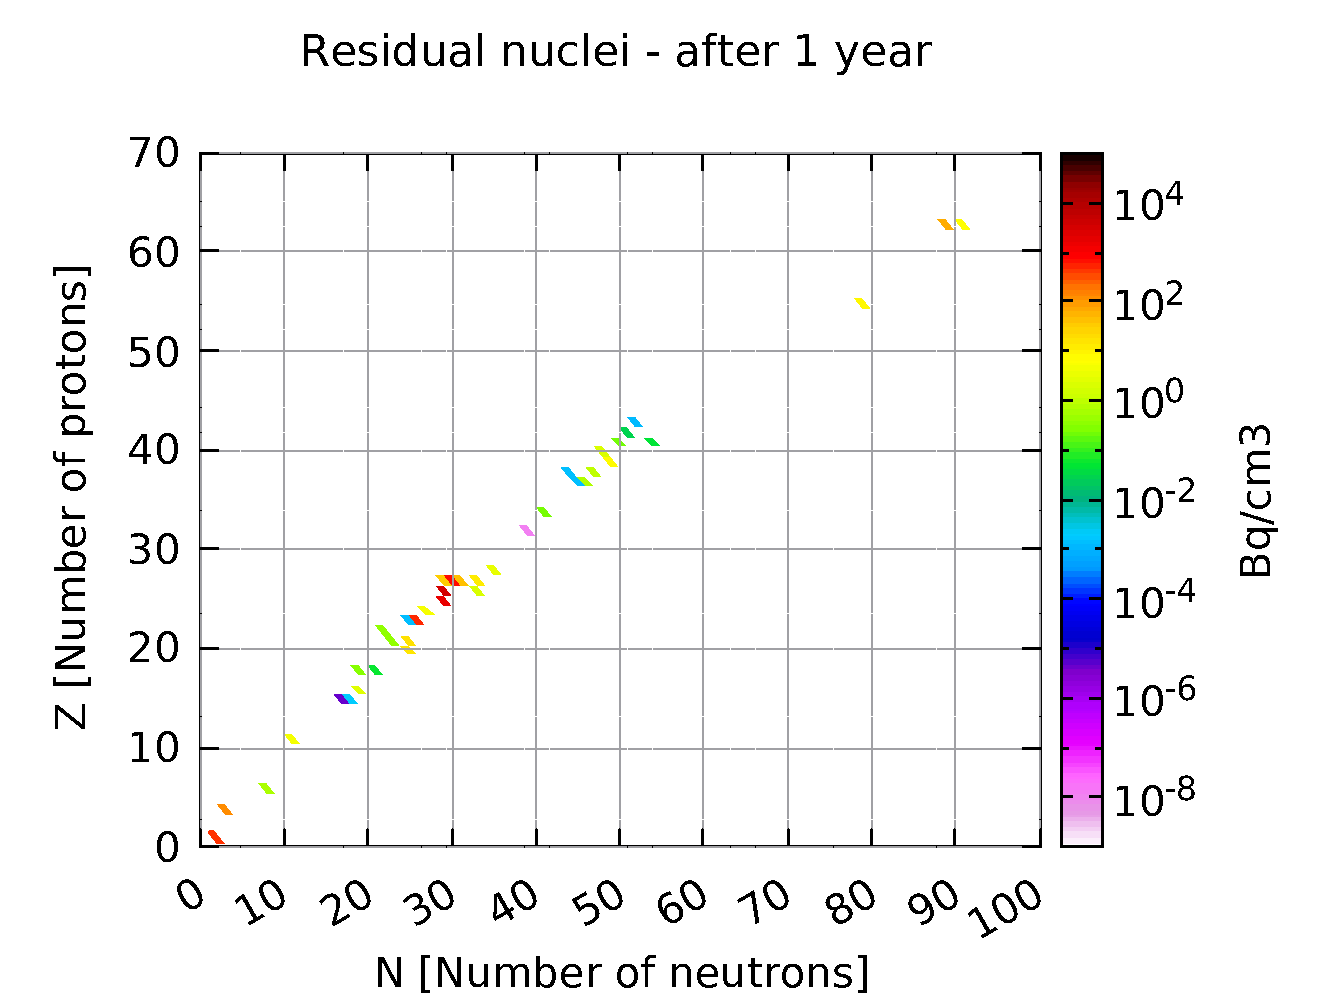
\includegraphics[width=0.6\textwidth]{Figures/BeamDump/Corrected_residualnuclei_plots/ResidualNuclei_Design2_5_correct_scale.pdf}
\caption[Residual nuclei in the ILC main beam dump after one year]{Chart of residual nuclei in the beam dump vessel and its surroundings after a cooling time of one year.
The axes show the number of protons (Z) and the number of neutrons (N) of the nuclei, from which the according element can be derived.
The color scale indicates the radioactivity in \si[detect-all]{\becquerel}/\si{\centi\meter\cubed} of the respective nuclei.}
\label{fig:BeamDumps:ResidualNuclei}
\end{figure}
\FloatBarrier
 
\subsection{Particle fluxes}
\label{BeamDumps:sim_surrounding:Particle}  
 Particle densities in the geometry can also be evaluated with \fluka, which is then given as the number of particles per \si{\centi\meter\cubed}.
 As an example, Figure~\ref{fig:BeamDumps:Electrons} shows the density distribution of electrons in the xz-plane for the two ILC beam dump designs.
 Since the primary beam also consists of electrons, the beam path is also visible coming from negative z along the beam pipe.
 Inside the water vessel, the beam is stopped and dissipated, and particle showers start forming. The electrons are boosted in the beam direction, because of which electrons outside the beam dump are mainly observed around and behind the vessel.  
\begin{figure}[!h]
 \centering
  \begin{subfigure}[b]{0.49\textwidth}
   \centering
    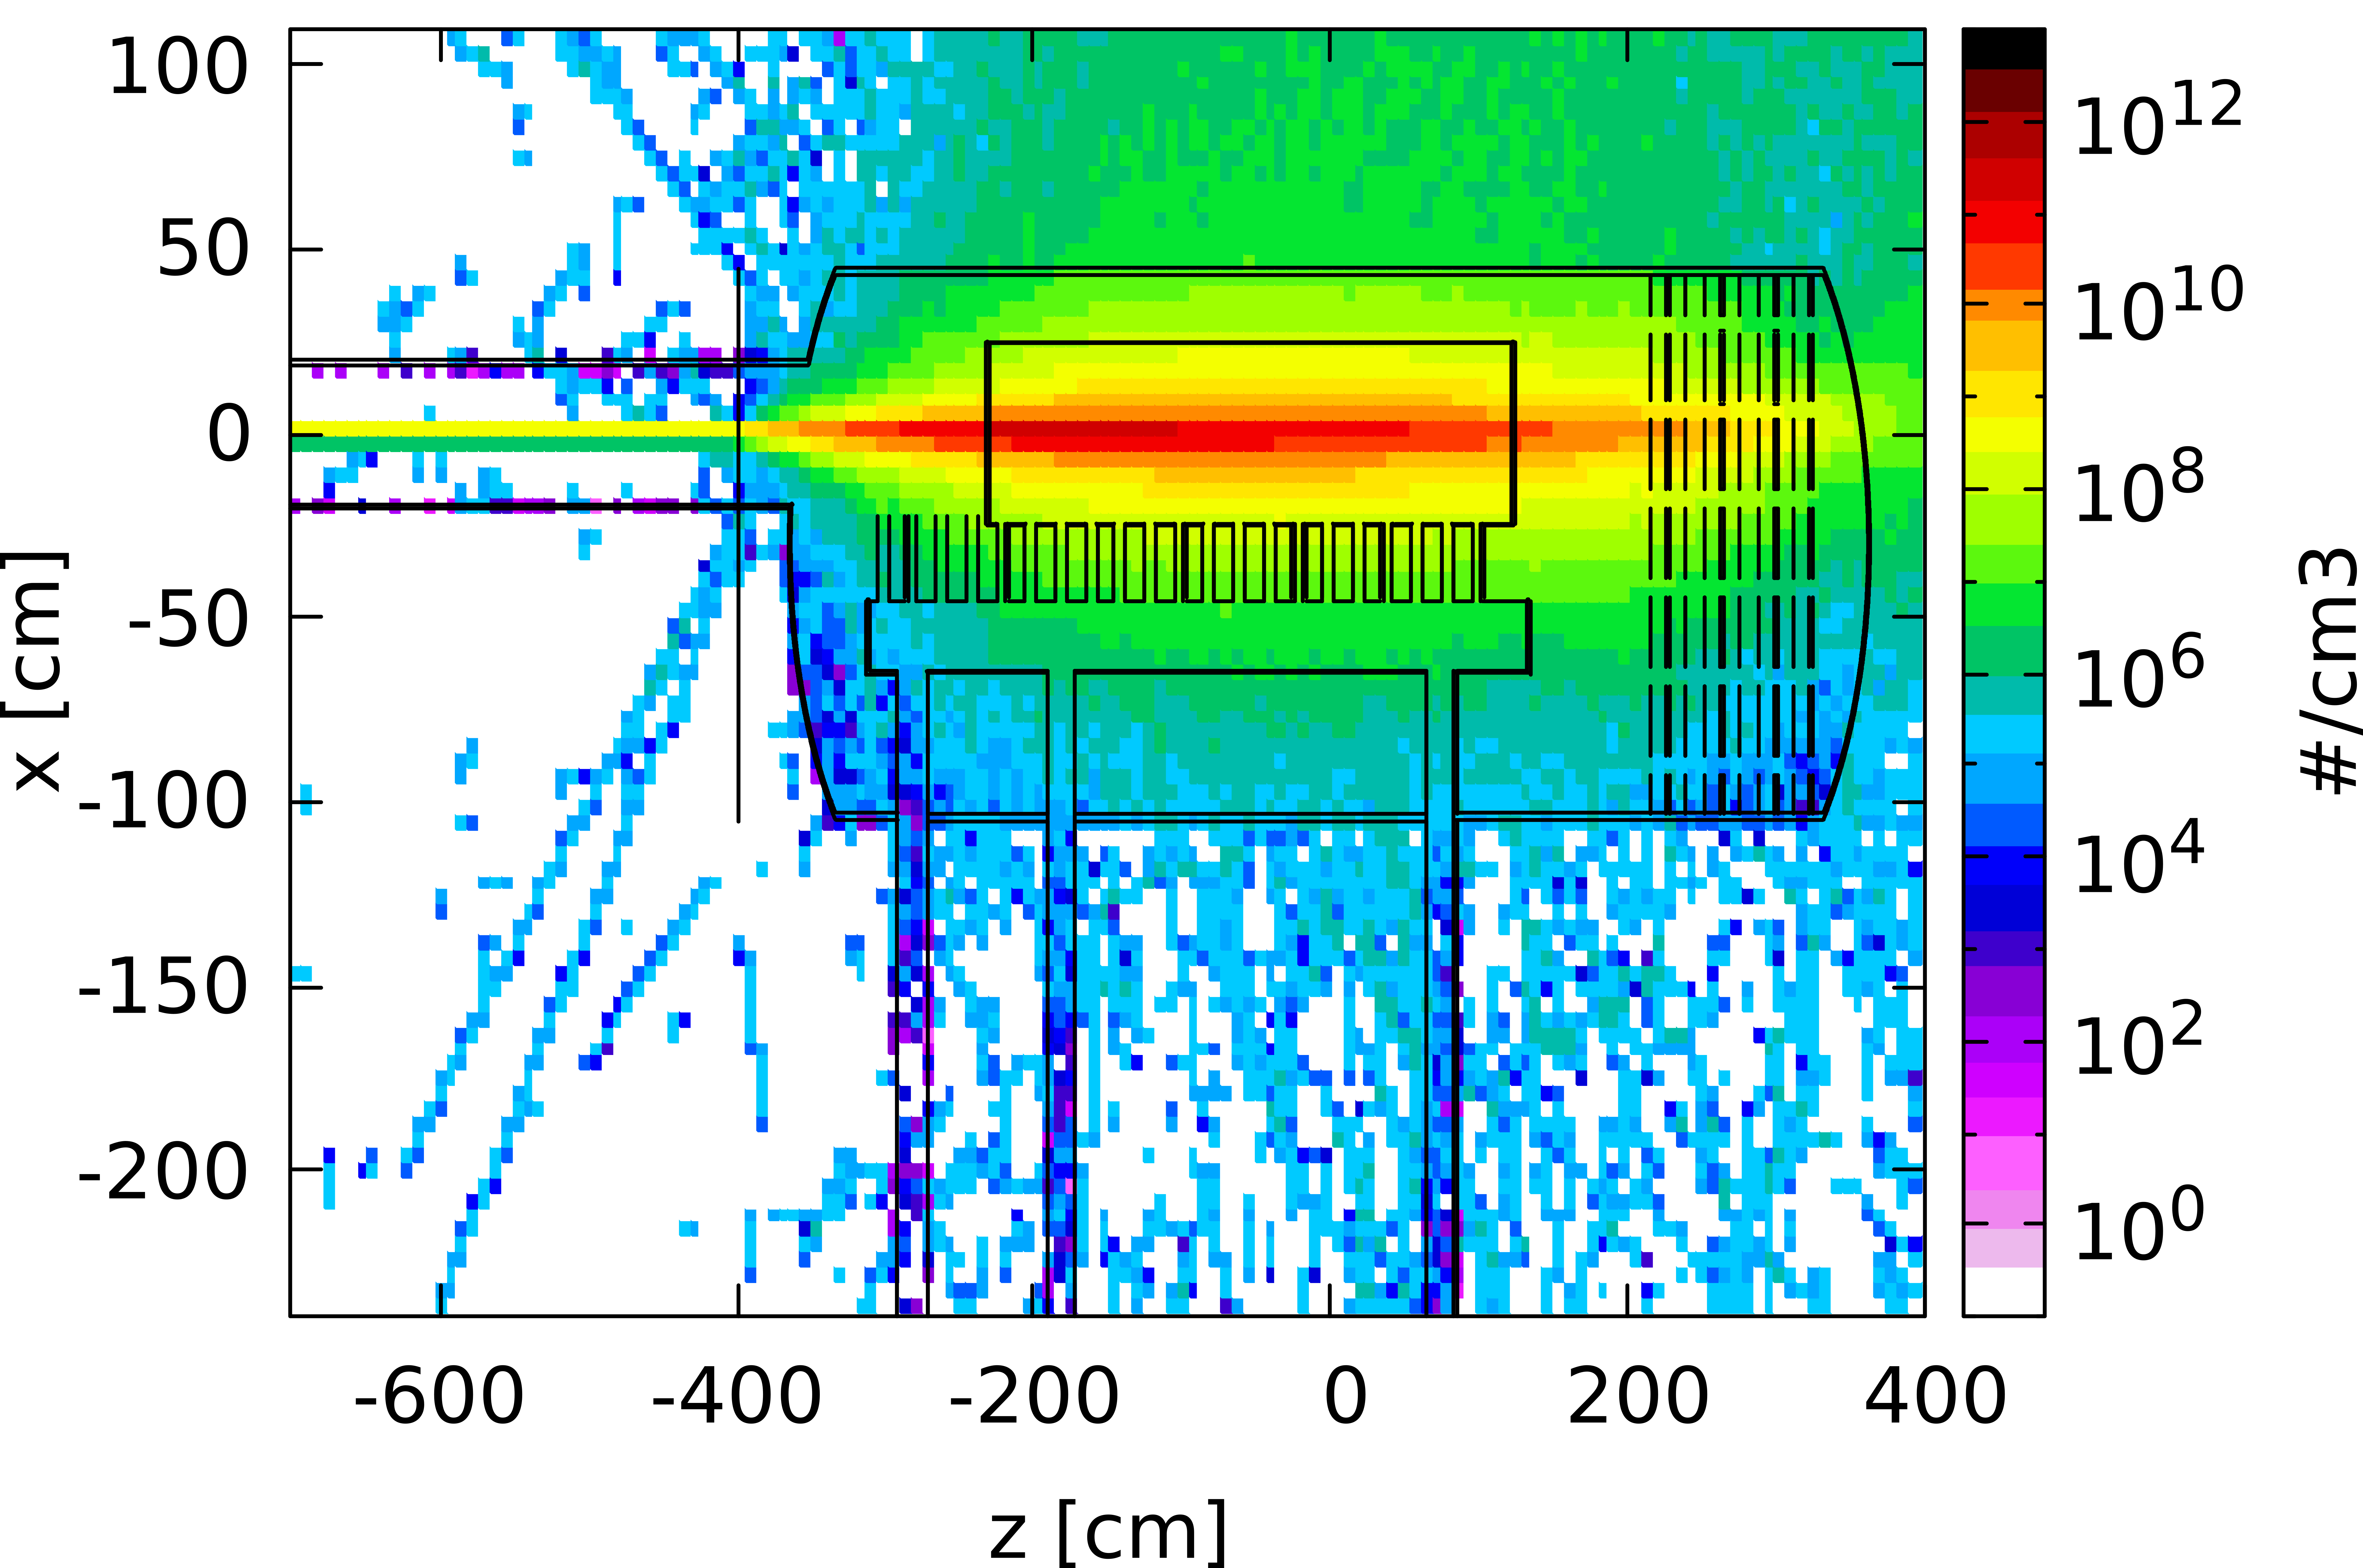
\includegraphics[width=\textwidth]{Figures/BeamDump/Electron_flux_xz_Design1.png}
   \caption{\designone}
   \end{subfigure}
   \hfill
    \begin{subfigure}[b]{0.49\textwidth}
   \centering
    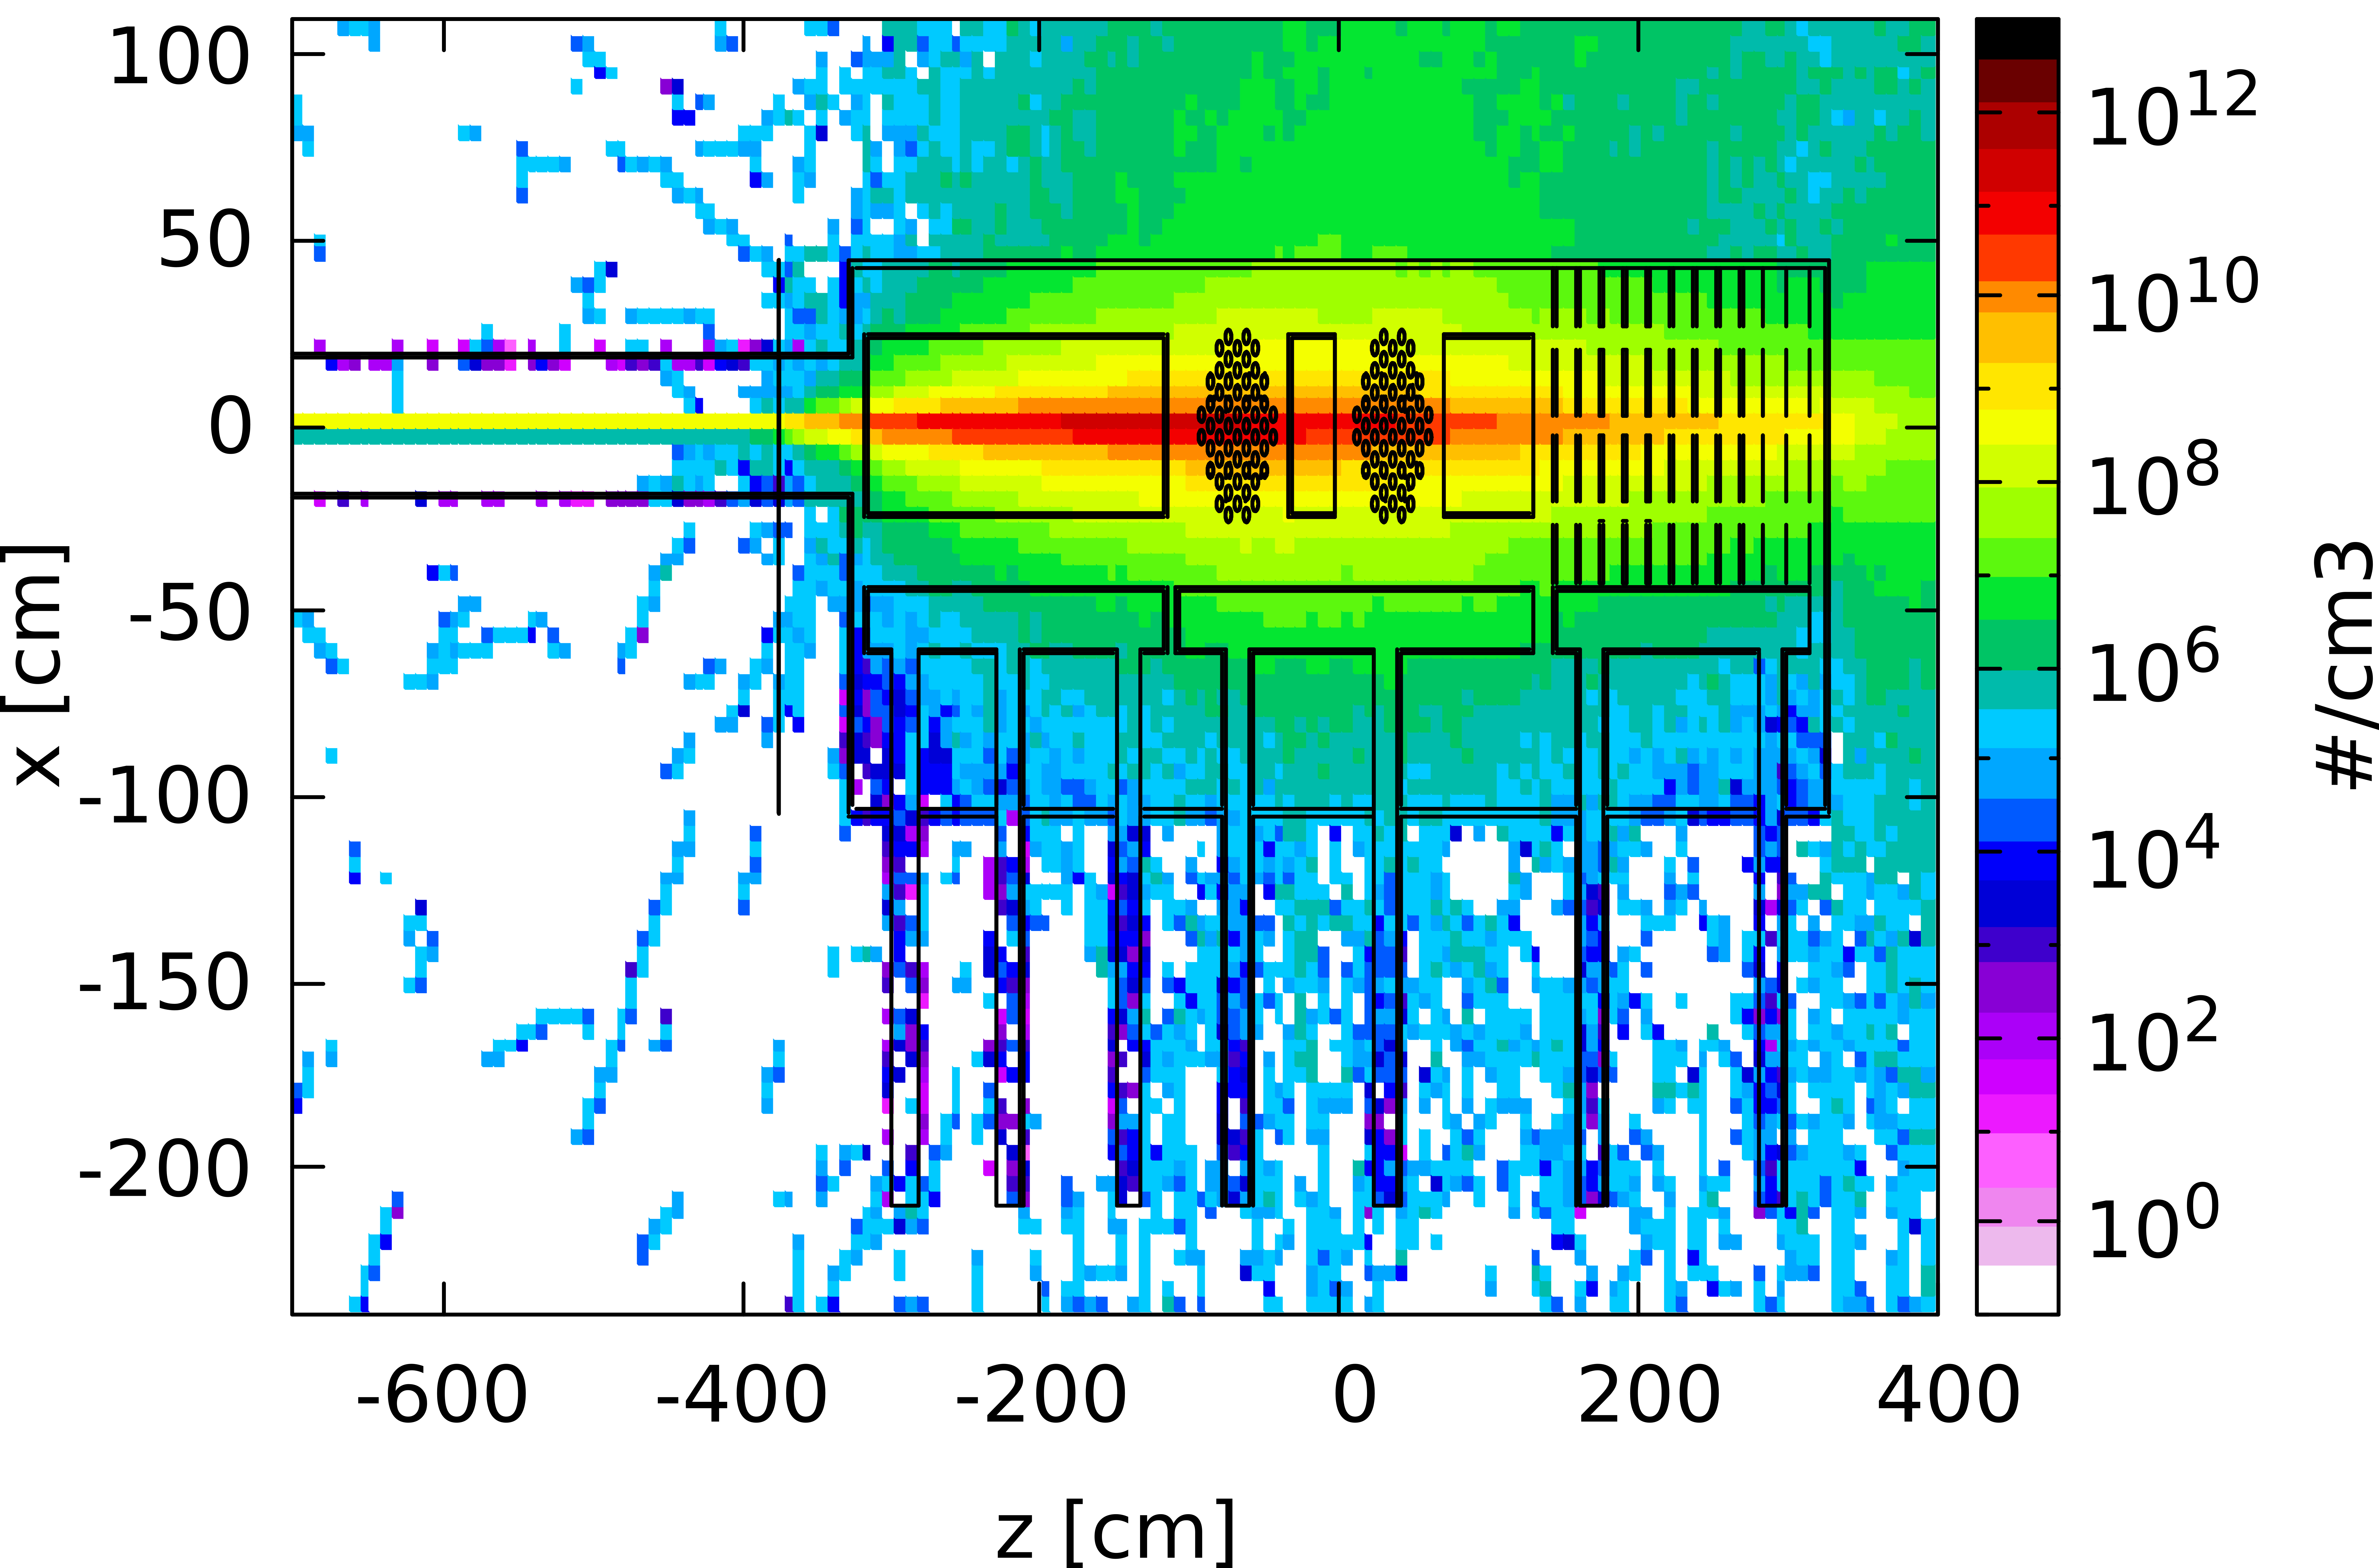
\includegraphics[width=\textwidth]{Figures/BeamDump/Electron_flux_xz_Design2.png}
   \caption{\designtwo}
   \end{subfigure}
   \caption[Electron flux in the ILC main beam dump]{\fluka result of the electron flux from one beam bunch in the ILC beam dump \designone (a) and \designtwo (b) and their surroundings.
   The view is in the xz-plane of the beam dump.
   The color scale shows the flux in number of particles per \si[detect-all]{\centi\meter\cubed} per bunch.}
   \label{fig:BeamDumps:Electrons}
\end{figure} 

This looks quite different for the neutron density distributions (Figure~\ref{fig:BeamDumps:Neutrons}).
 The primary electron beam undergoes the electromagnetic particle showers in the beam dump, which is desired in order to absorb the beam power.
 The produced secondary particles from the particle showers, however, interact with the beam dump material and the water via ionization and photonuclear processes.
 The products from these processes are neutrons in connection with the radioactive nuclei discussed in Section~\ref{BeamDumps:sim_surrounding:Dose}.
 Due to the way the neutrons are produced, they can be found under every solid angle, hence also in the backward direction.
 Since the neutron flux outside the vessel does not show a significant difference between \designone and \designtwo, the following results are shown for \designone only.
 They are however valid for both designs.
\begin{figure}[!h]
 \centering
  \begin{subfigure}[b]{0.49\textwidth}
   \centering
    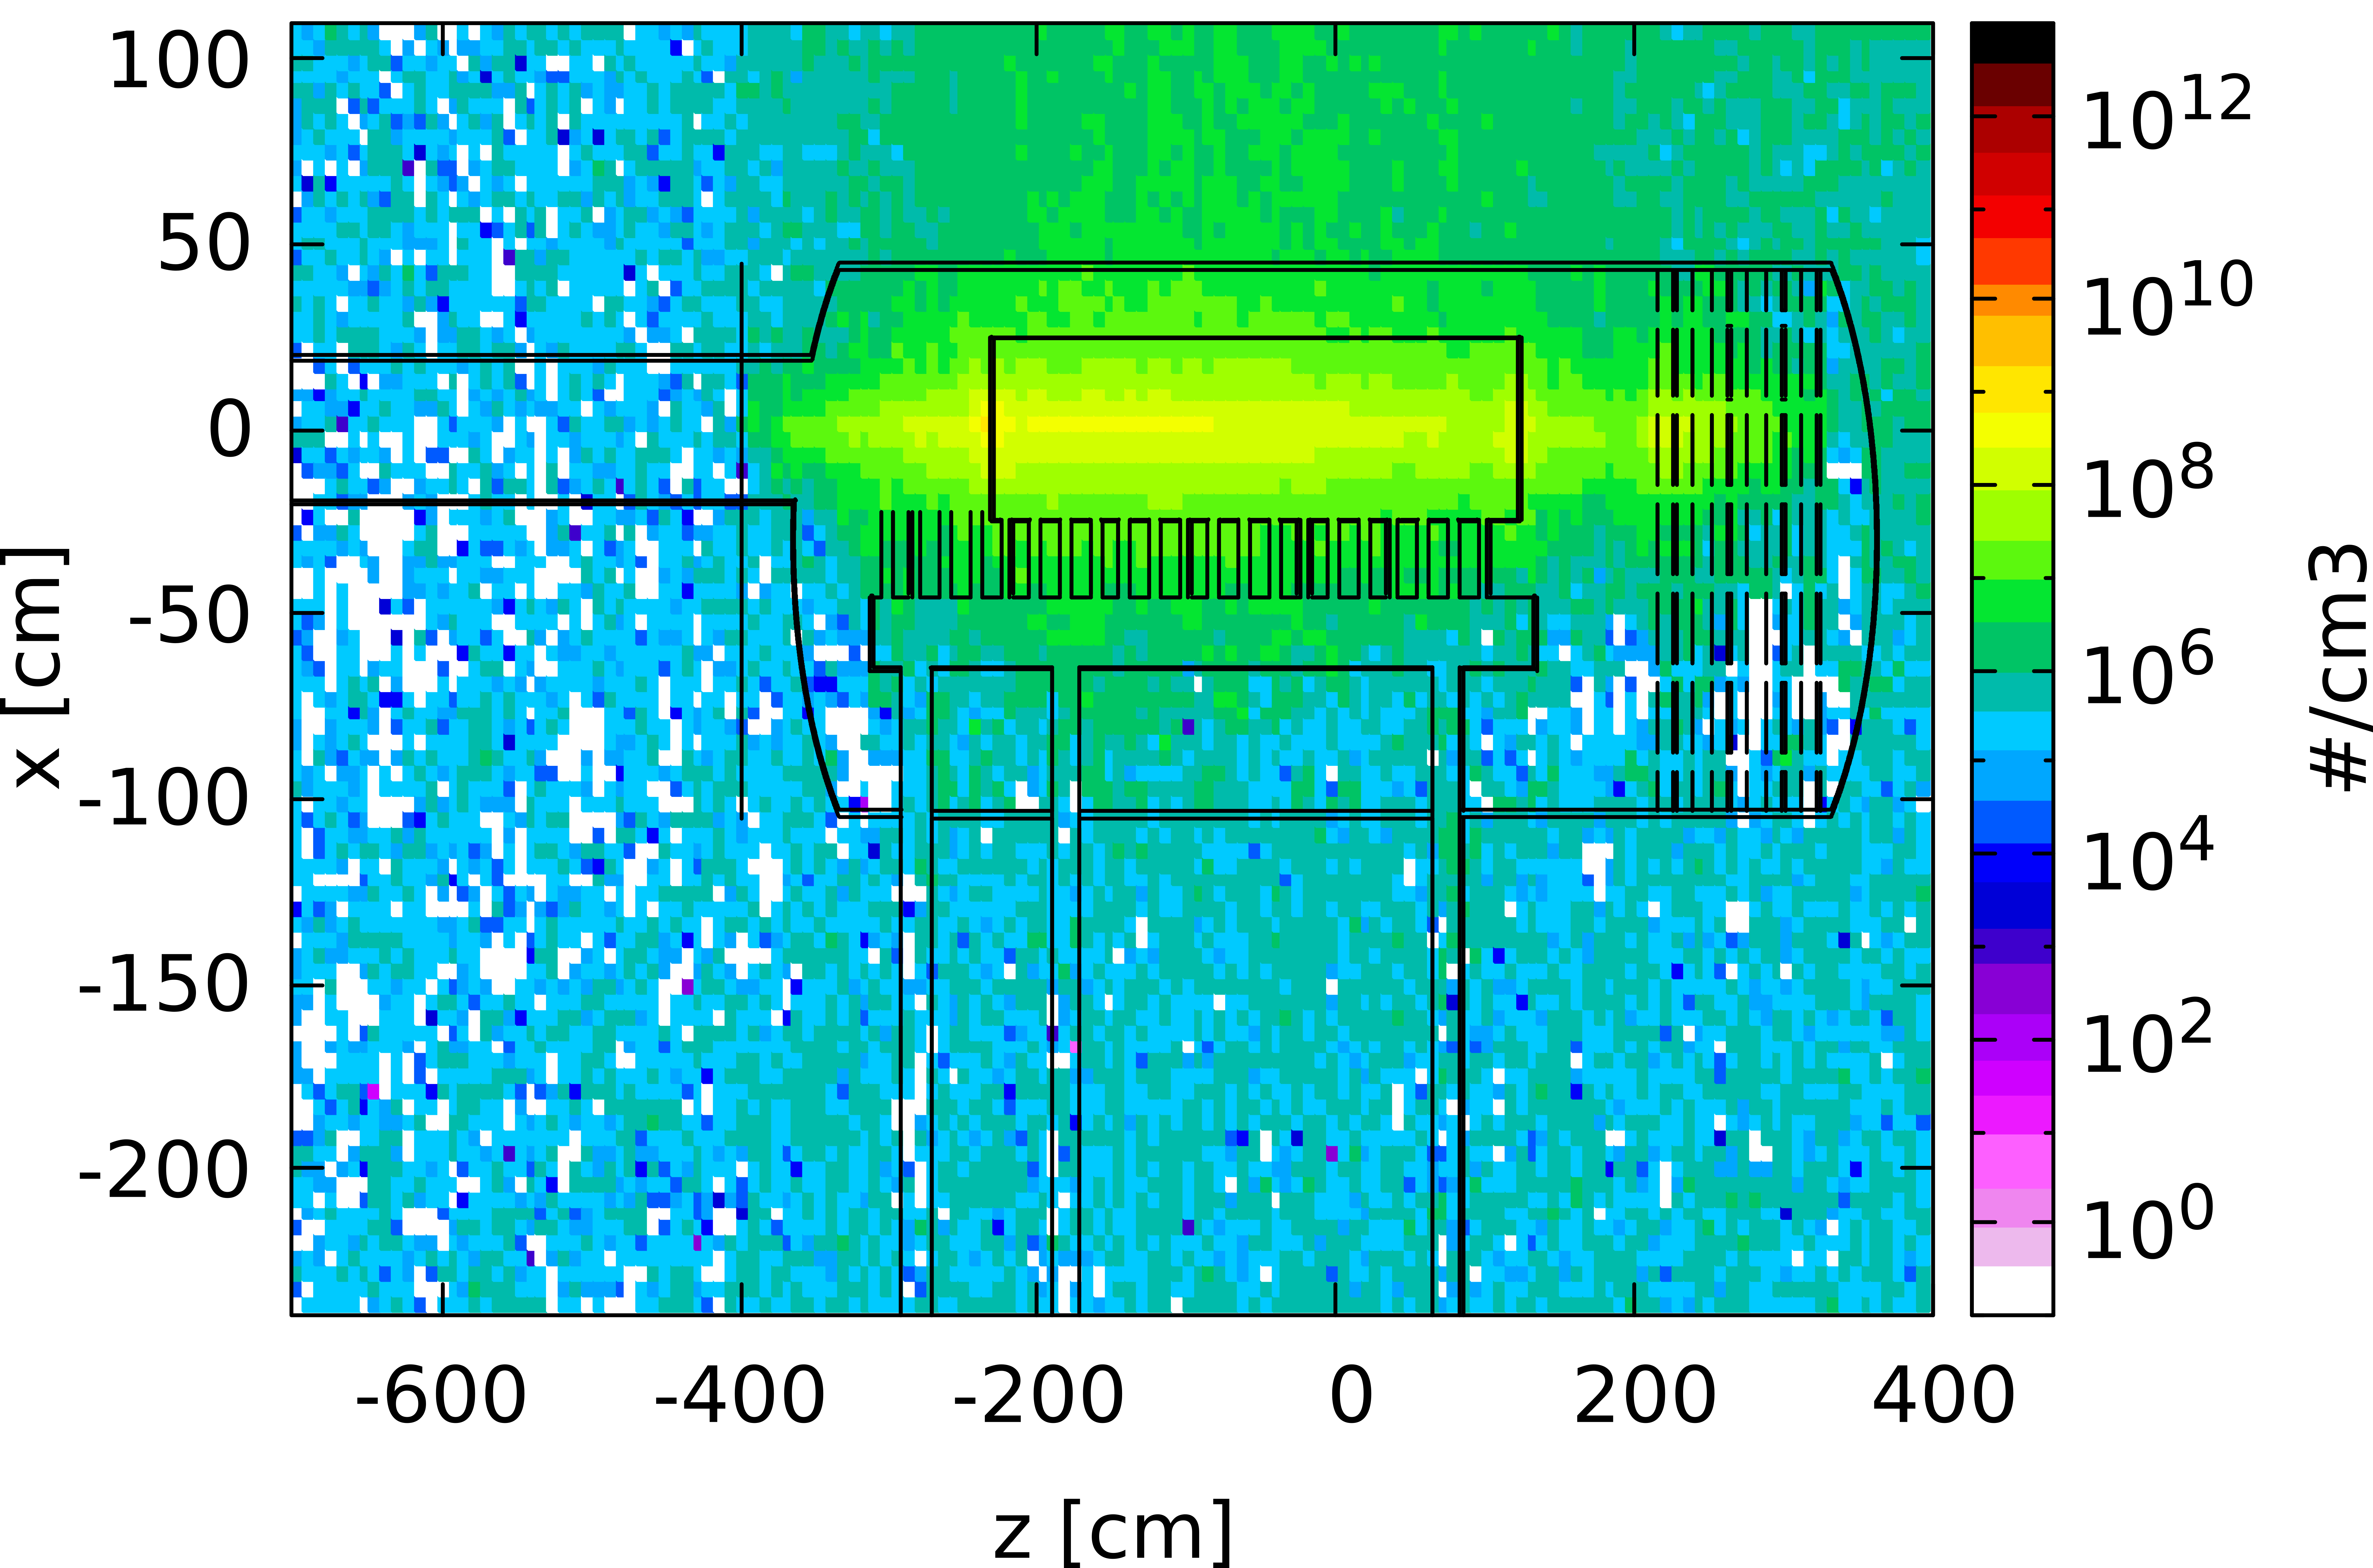
\includegraphics[width=\textwidth]{Figures/BeamDump/Neutron_flux_xz_Design1.png}
   \caption{\designone}
   \end{subfigure}
   \hfill
    \begin{subfigure}[b]{0.49\textwidth}
   \centering
    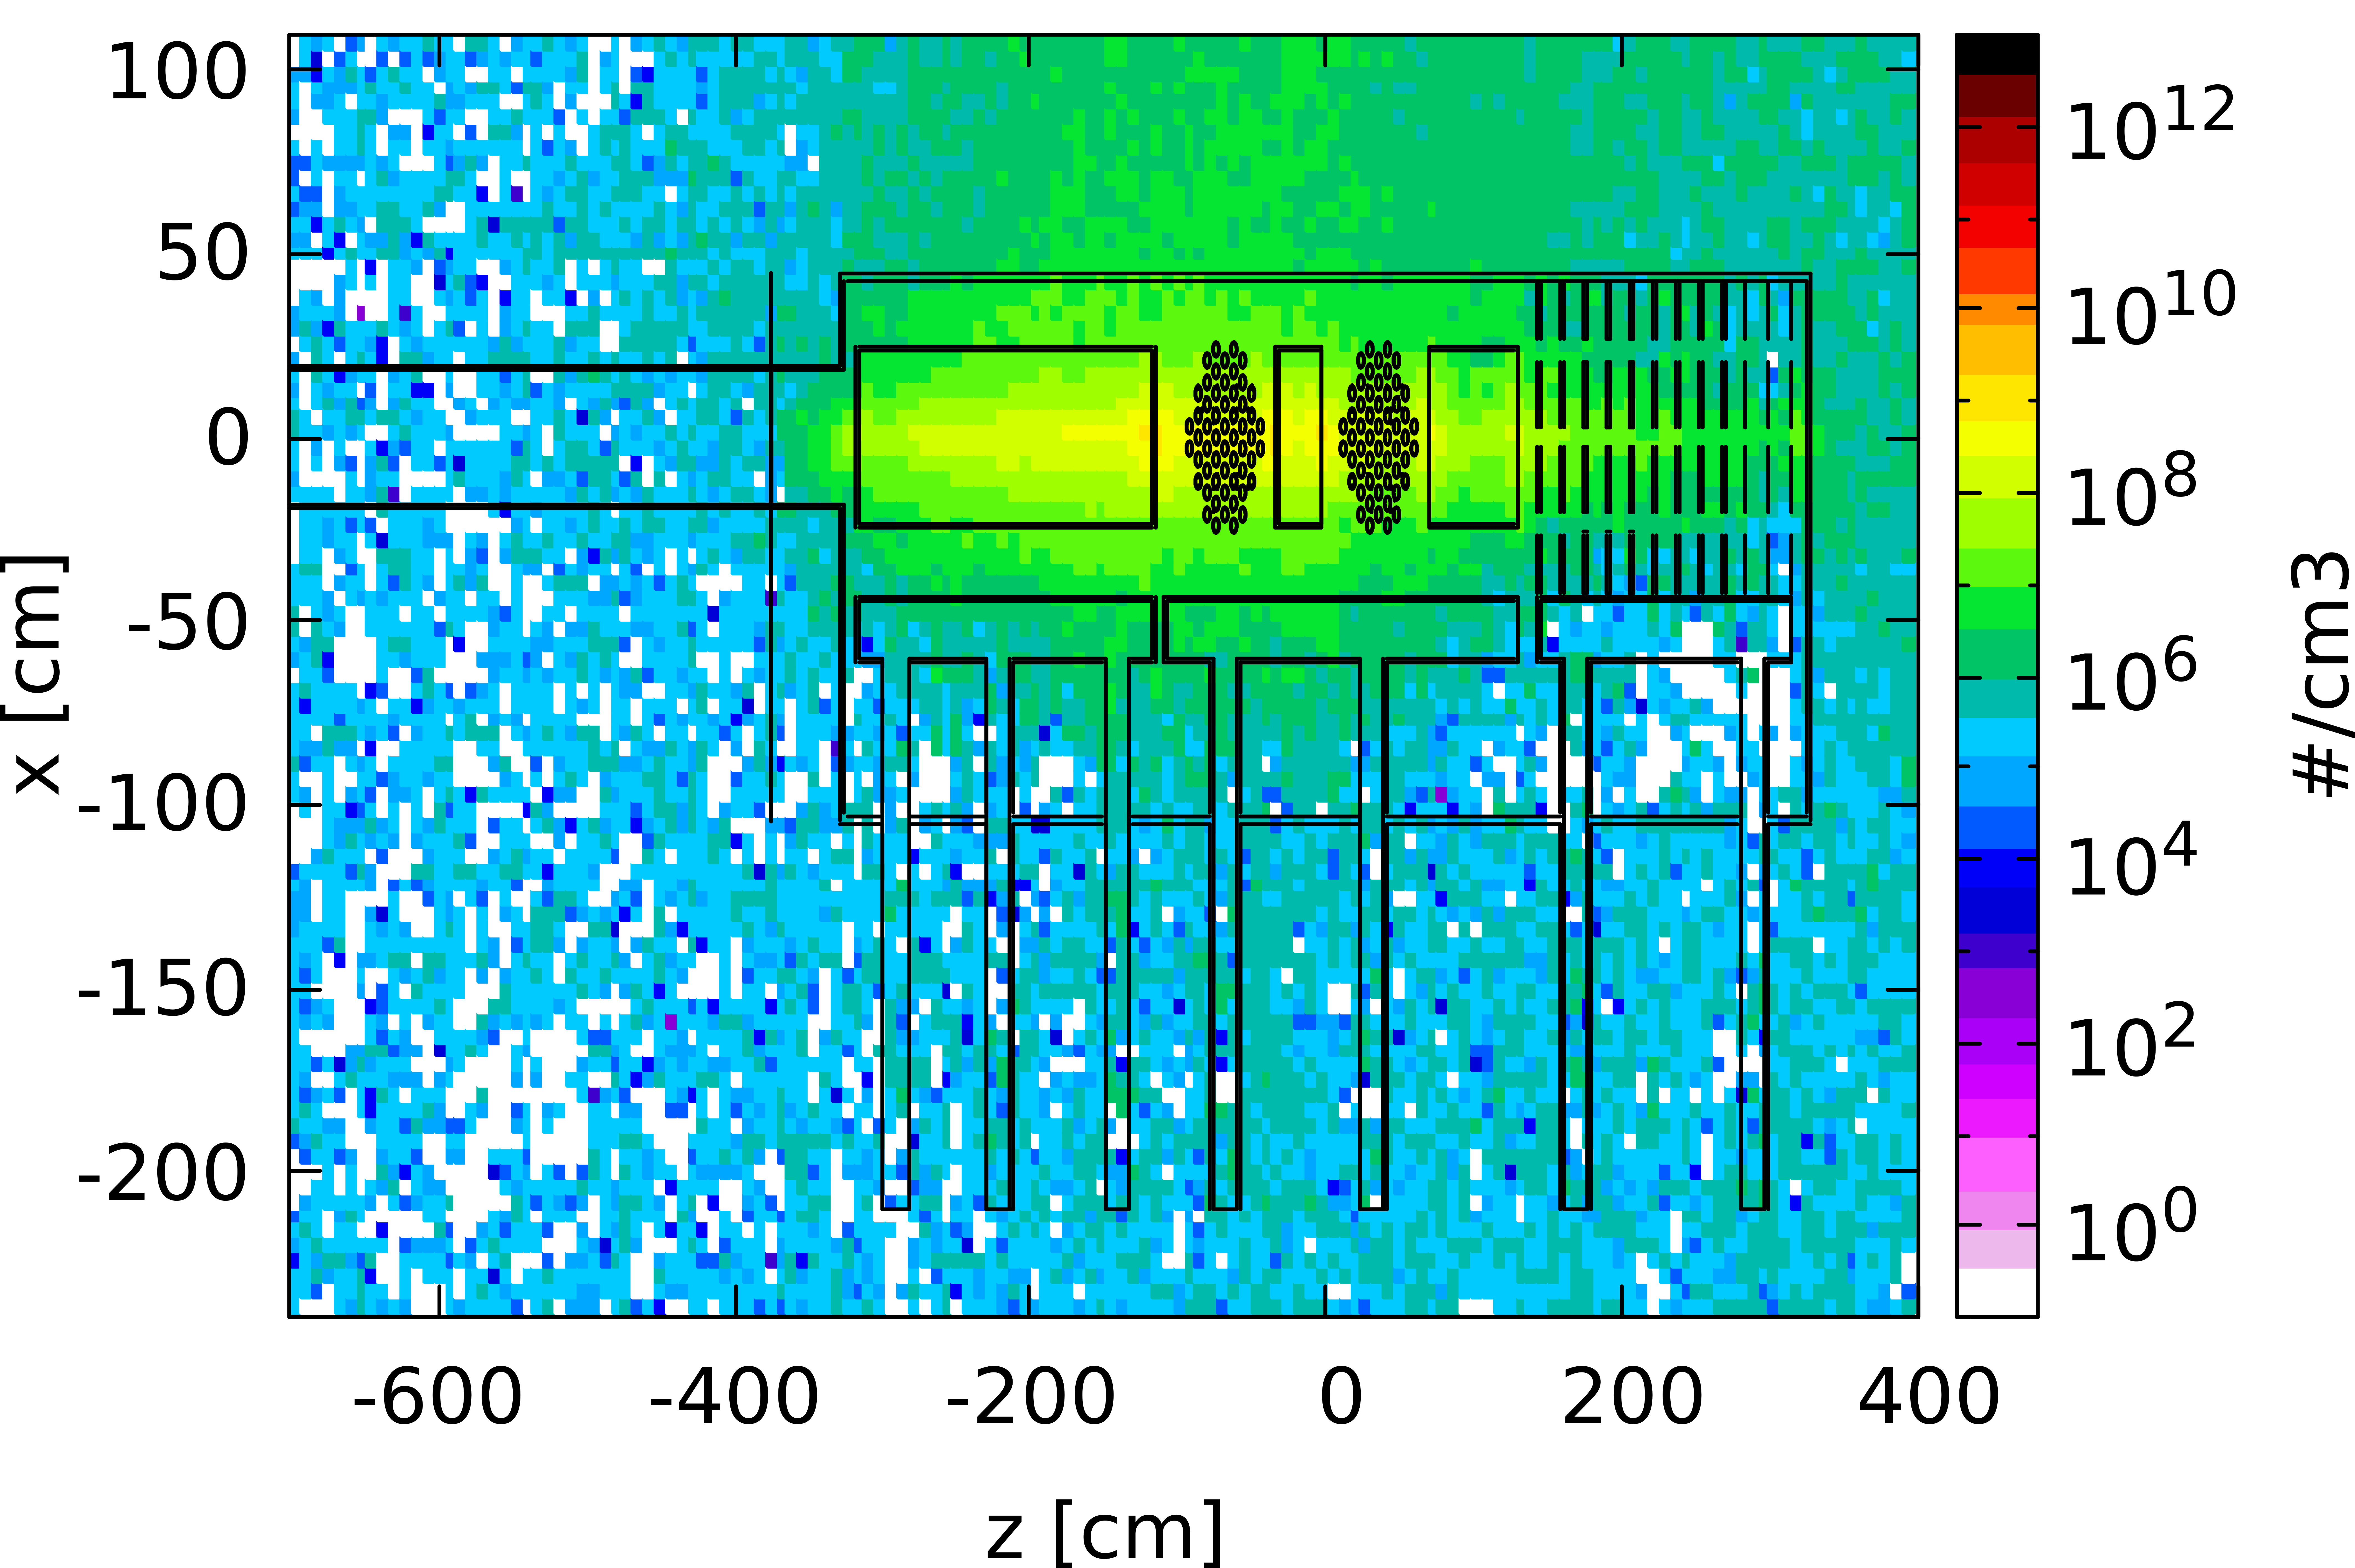
\includegraphics[width=\textwidth]{Figures/BeamDump/Neutron_flux_xz_Design2.png}
   \caption{\designtwo}
   \end{subfigure}
   \caption[Neutron flux in the ILC main beam dump]{\fluka result of the neutron flux from one beam bunch in the ILC beam dump \designone (a) and \designtwo (b) and their surroundings.
   The view is in the xz-plane of the beam dump.
   The color scale shows the flux in number of particles per \si[detect-all]{\centi\meter\cubed} per bunch.}
   \label{fig:BeamDumps:Neutrons}
\end{figure} 
\\By adding an imaginary scoring plane\footnote{Designated plane in the \fluka geometry model, at which physical quantities can be measured.} upstream of the beam dump vessel as indicated in Figure~\ref{fig:BeamDumps:NeutronScoring} (a), the neutrons escaping the beam dump in the direction of the extraction line can be counted.
\fluka then recorded the kinetic energy of the neutrons crossing this scoring plane under various angles to the z-axis.
The energy spectra can be seen in Figure~\ref{fig:BeamDumps:NeutronScoring} (b).
The spectra range from about \SI{1}{\meV} to \SI{500}{\MeV}, and indicate the number of neutrons under different angles. 
The graph ``0 - 45 degrees'' shows the energy spectrum for all neutrons crossing the boundary in the direction of the extraction line (the negative z-direction) under an angle of up to \SI{45}{\degree}.
The energy spectrum of the neutrons that cross the boundary under an angle between \SI{45}{\degree} and \SI{90}{\degree} to the negative z-direction is also displayed in Figure~\ref{fig:BeamDumps:NeutronScoring} (b).
The combination of both spectra is shown by the red graph, indicated with ``all angles'' in the figure legend.
The first peak in the meV range represents the thermal neutron energy peak.
At the eV range, resonance peaks from resonant elastic scattering of neutrons with a compound nucleus are visible.
These resonance peaks are element specific, so that the peaks indicate which materials the neutrons have interacted with.
%See email from Vasilis on 16.April ~12Uhr
The peaks visible in the plot mainly originate from elastic neutron scattering processes with iron and copper atoms, which leads to resonances in the neutron cross section at around \num{e-2} to \SI{e-1}{\MeV}~\cite{neutron_resonances,neutron_resonances2}.
Finally in the range of $\sim$\SI{100}{\MeV}, the so-called evaporation or fission peak of fast neutrons is visible.

All the neutrons that pass the scoring plane are oriented in the direction of the extraction line and hence in the direction of the interaction region and the detectors.
As can be seen in Section~\ref{BeamDumps:sim_EXT}, the neutrons do not reach the detectors freely.
Due to shielding walls and extraction line components, the number of neutrons is reduced.
\begin{figure}[hbp]
\centering
  \begin{subfigure}[b]{0.4\textwidth}
   \centering
    \raisebox{12mm}{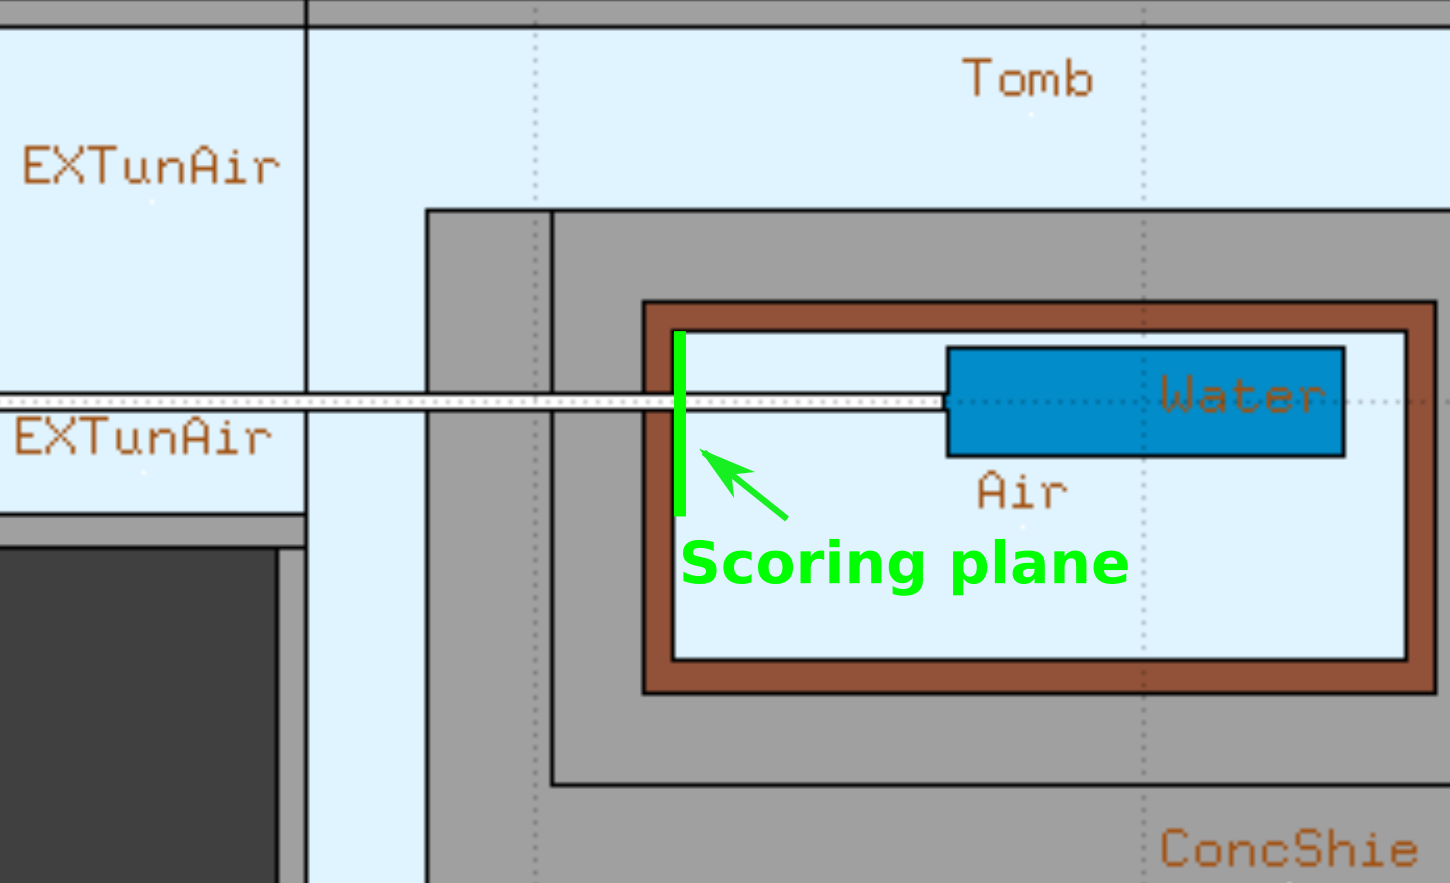
\includegraphics[width=0.99\textwidth]{Figures/BeamDump/Bird_view_BeamDump_Tomb_ScoringPlane.png}}
   \caption{Neutron scoring plane}
   \end{subfigure}
   \hfill
    \begin{subfigure}[b]{0.59\textwidth}
   \centering
    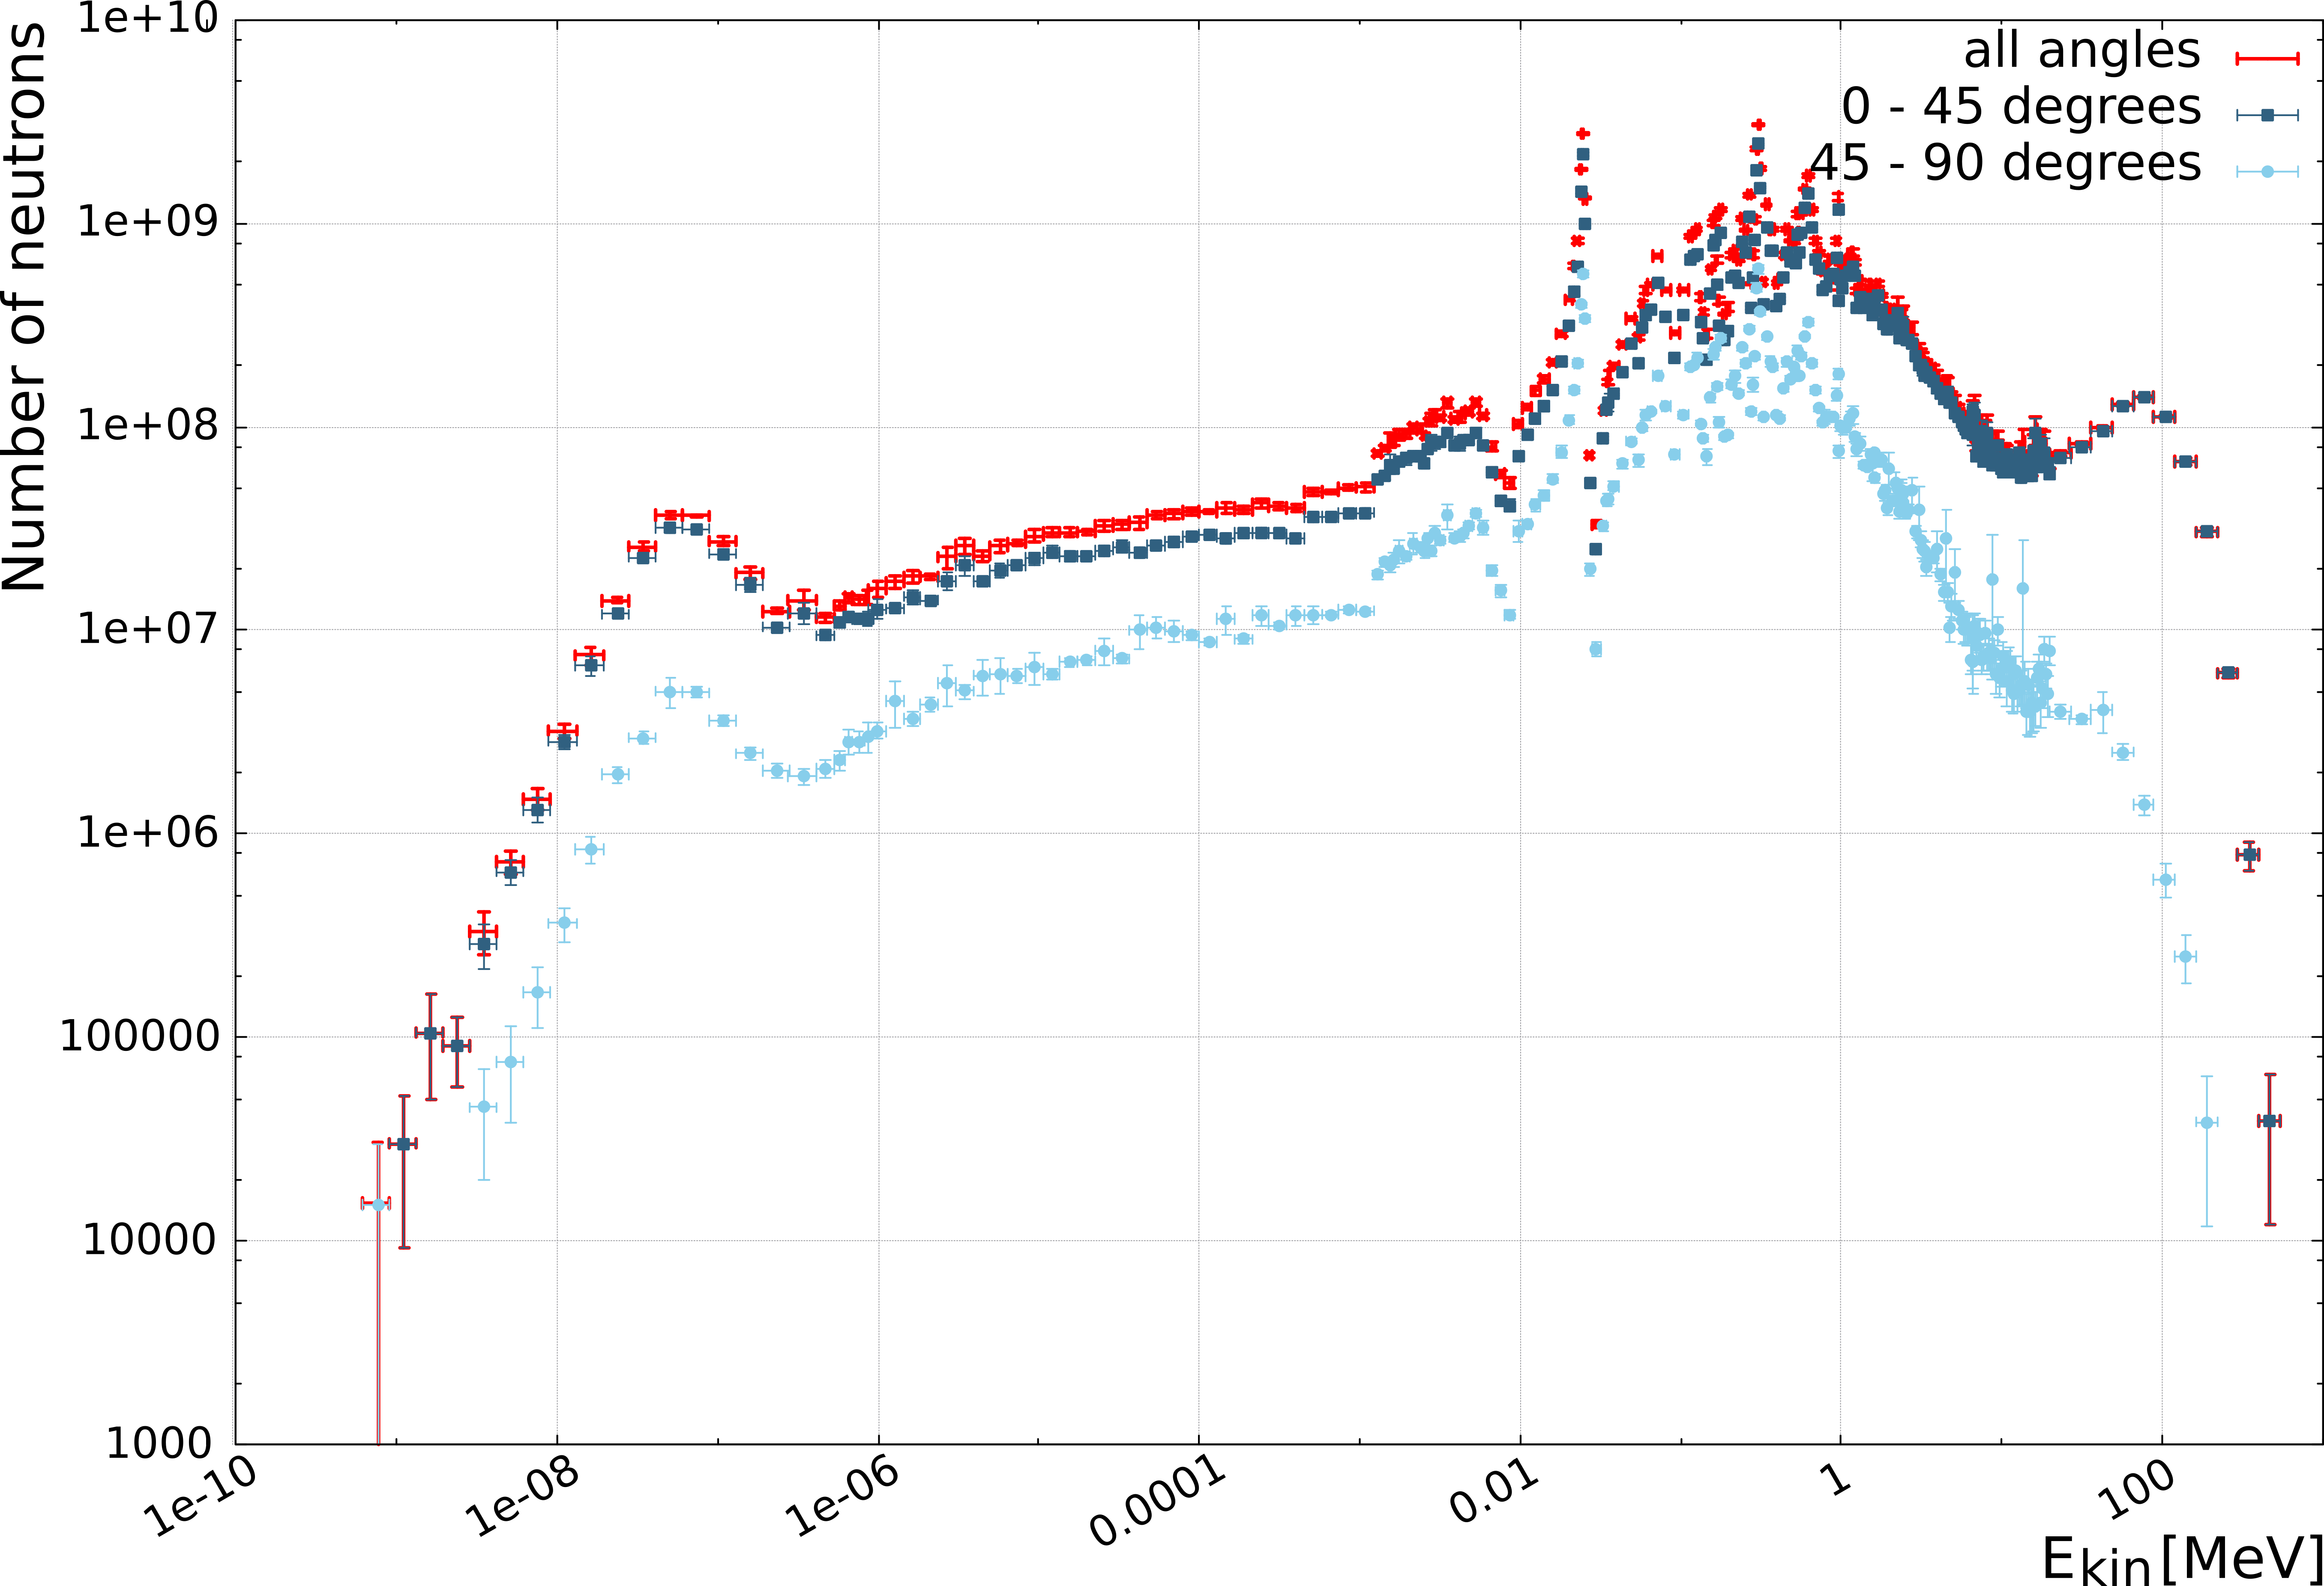
\includegraphics[width=\textwidth]{Figures/BeamDump/Neutron_spectrum_final_BeamDump_hall.png}
   \caption{Neutron energy distribution}
   \end{subfigure}
\caption[Neutron scoring plane in the main beam dump hall]{Scoring neutrons escaping the beam dump vessel in the direction of the extraction line.
\\Figure (a) shows the position of the scoring plane in \fluka in the xz-view of the beam dump hall.
At the boundary of the scoring plane, the neutron energy spectrum is recorded.
\\Figure (b) shows the energy spectra of the neutrons, which are produced in the beam dump \designone from one ILC beam bunch, and which cross the scoring plane indicated in Figure (a).
The different graphs stand for different crossing angles to the z-axis.
The red graph (``all angles'') is the combination of the other two graphs (``0 - 45 degrees'' and ``45 - 90 degrees'').}
\label{fig:BeamDumps:NeutronScoring}
\end{figure}

\clearpage
\section{Simulation studies of the extraction line}
\label{BeamDumps:sim_EXT}

The neutrons, which are created in the ILC beam dumps and directed towards the interaction region, are not freely traveling through the extraction line.
As mentioned before, the extraction line lattice consists of magnets and collimators, which for the neutrons represent shielding obstacles.
An accelerator lattice is the sequence of all beam line components.
\\The first device of the extraction line lattice is the focusing quadrupole QDEX1, closest to the IP.
Like the last quadrupole QD0 of the final-focus system, QDEX1 is also an integrated part of the two detector experiments.
Since the neutrons escaping the extraction line shall be input to a full detector simulation, the \fluka model of the EXT line therefore does not include QDEX1.
The model rather ends at \SI{9.3}{\meter} from the IP, which will then be the starting point of the escaping neutrons for the following \geant simulation of the \sid detector.
The component of the \fluka model closest to the IP is the cryostat containing QFEX2A, the only other superconducting magnet of the EXT lattice next to QDEX1.
The cryostat is followed by 13 quadrupole models, which prepare the spent beams for diagnostic measurements and which shall prevent any beam loss~\cites[p. 139 ff]{TDR32}{EXT_design, EXT_design2}.
The following eight dipole magnets are part of the energy diagnostic section.
The polarimeter section containing four dipole magnets, measures the polarization level of the beam.
Finally, the collimators located at various positions along the EXT line are protection collimators, shielding the beam line devices from irradiation.
\begin{figure}[!b]
 \centering
  \begin{subfigure}[b]{\textwidth}
   \centering
    
\includegraphics[width=\textwidth]{Figures/BeamDump/EXT_line.png}
   \caption{Full extraction line}
   \end{subfigure}\\
   \begin{subfigure}[b]{0.63\textwidth}
   \centering
    \includegraphics[width=\textwidth]{Figures/BeamDump/EXT_line_1.png}
   \caption{Zoom of the first magnet section}
   \end{subfigure}
   \hfill
    \begin{subfigure}[b]{0.35\textwidth}
   \centering
    \includegraphics[width=\textwidth]{Figures/BeamDump/EXT_line_2.png}
   \caption{3D-view of the dipole magnets}
   \end{subfigure}
   \caption[\fluka model of the ILC extraction line]{Pictures of the ILC extraction line, modeled within \flair.
   The full model is shown in a xz-view in Figure (a).
   Figures (b) and (c) show closeup views of the magnet section in the beginning of the extraction line.}
   \label{fig:BeamDumps:EXT}
\end{figure} 
\\The goal of this \fluka simulation is to obtain the number and the distribution of neutrons reaching the detectors.
The models of the EXT line components are therefore simplified models aimed at representing the shielding objects with the correct sizes and positions along the line.
The beam line infrastructure, like vacuum pumps and valves are not accounted for in the simulation.
Figure~\ref{fig:BeamDumps:EXT} shows the \fluka model of the extraction line.

\begin{figure}[!t]
\centering
  \begin{subfigure}[b]{\textwidth}
   \centering
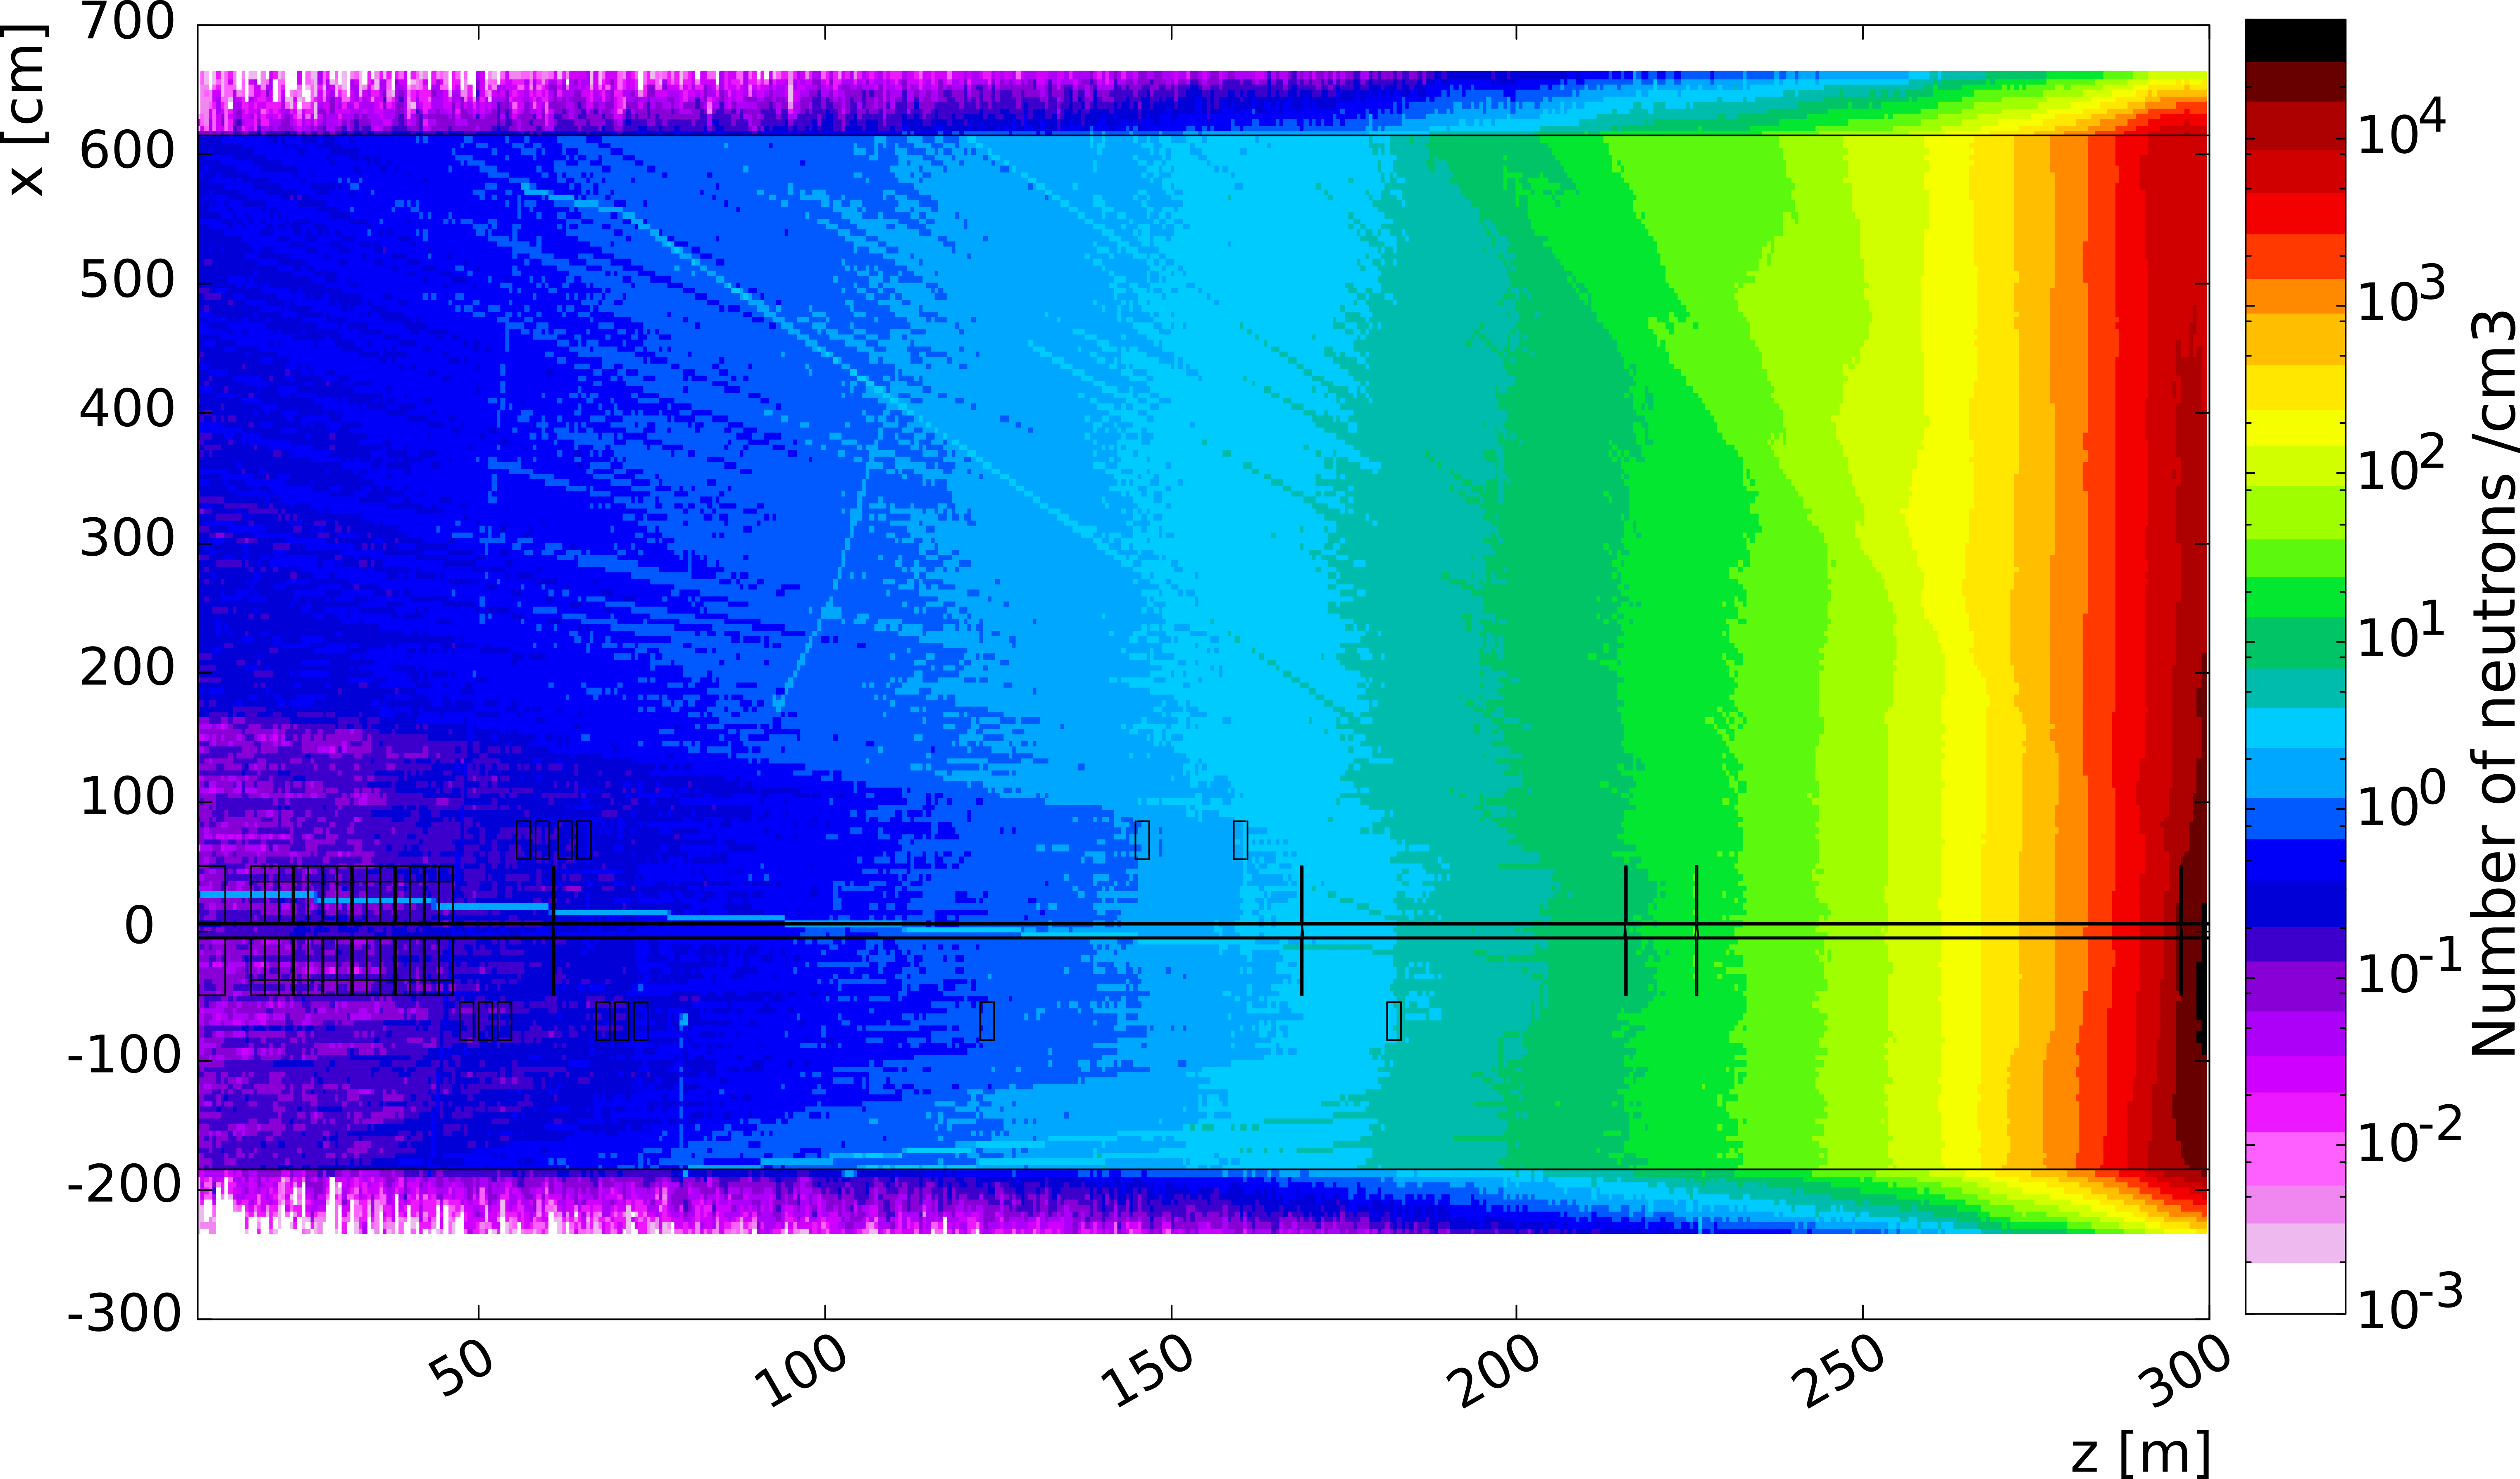
\includegraphics[width=0.88\textwidth]{Figures/BeamDump/Neutron_dis_in_full_EXT_tunnel.png}
\caption{Neutron density distribution}
   \end{subfigure}\\
    \begin{subfigure}[b]{\textwidth}
   \centering
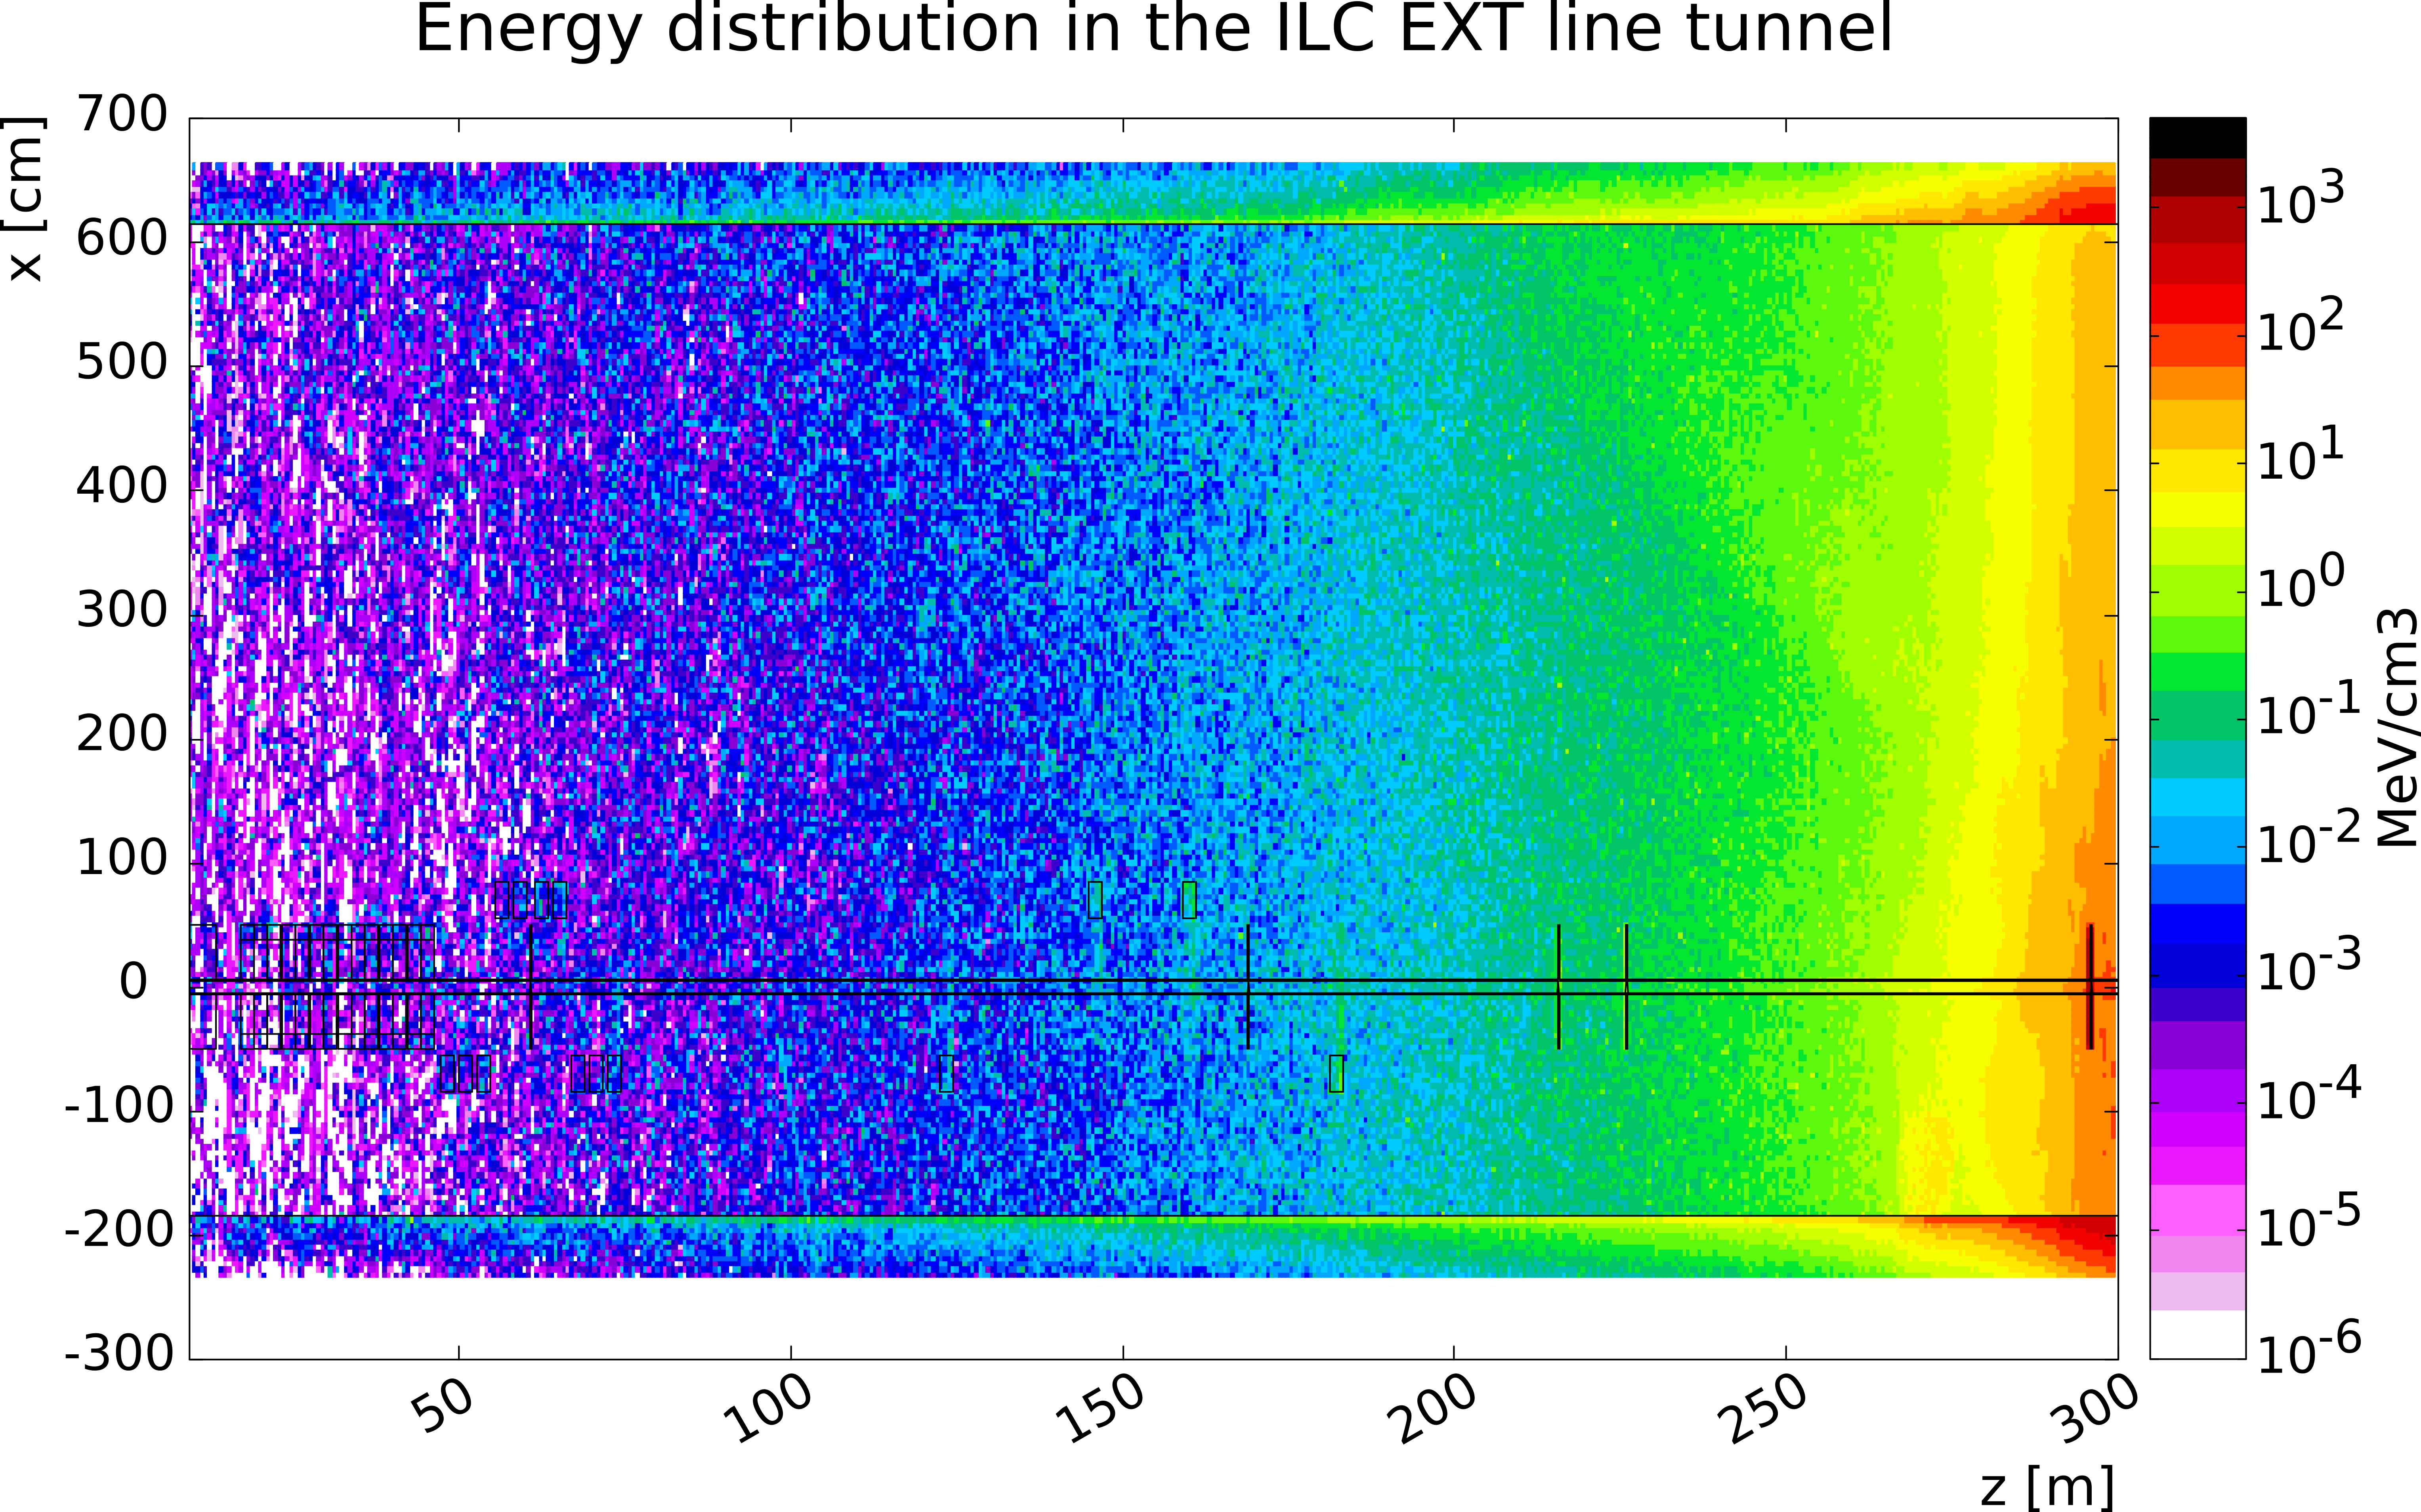
\includegraphics[width=0.88\textwidth]{Figures/BeamDump/Energy_dis_in_full_EXT_tunnel.png}
\caption{Deposited energy distribution}
\end{subfigure}
\caption[Spatial distribution of the neutron density and the deposited energy in the ILC extraction line tunnel]{
Figure (a) shows the spatial distribution of the neutrons in the ILC extraction line tunnel simulated with \fluka.
The color scale shows the number of neutrons per unit area, normalized to the rate resulting from one ILC beam bunch dumped in the water vessel.
\\Figure (b) shows the spatial distribution of the deposited energy in the ILC extraction line tunnel simulated with \fluka.
The color scale shows the deposited energy in \si[detect-all]{\MeV} per unit area, normalized to the results from one ILC beam bunch dumped in the water vessel.}
\label{fig:BeamDumps:NeutronEnergy_dis_EXT}
\end{figure}
\FloatBarrier
The tunnel stretches from \SI{9.3}{\meter} from the IP to \SI{300}{\meter}, where the entrance to the beam dump hall is located.
It has a width of \SI{8}{\meter}.
\\The design and locations of the beam line components are taken from the most recent ILC lattice drafts~\cite{EXT_lattice,EXT_lattice2}.
The magnets are simulated without their respective magnetic field maps, since the neutron tracks are not affected by magnetic fields.
The neutrons, which reach the extraction line past the beam dump shielding walls, are tracked through the extraction line geometry described above.
The resulting neutron density in the tunnel is shown in Figure~\ref{fig:BeamDumps:NeutronEnergy_dis_EXT} (a) in a view of the xz-plane.
Close to the beam dump hall, at around z = \SI{300}{\meter}, the neutron density reaches over \SI{e4}{\per\centi\meter\cubed}.
This density sinks to about \SI{1}{\per\centi\meter\cubed} close to the interaction region at z = \SI{9.3}{\meter}.
The beam line components shield the neutron flux such that the neutron density between about \SI{-200}{\centi\meter} and \SI{200}{\centi\meter} in x is reduced to about \SI{0.1}{\per\centi\meter\cubed}.
\\The resulting deposited energy is shown in the xz-plane in Figure~\ref{fig:BeamDumps:NeutronEnergy_dis_EXT} (b).
Due to the high density of neutrons close to the beam hall, the energy density here reaches up to 
\num{e2} - \SI{e3}{\MeV\per\centi\meter\cubed}.
Also according to the neutron density distribution, the deposited energy close to the interaction region drops to about \num{0.1} - \SI{1}{\keV\per\centi\meter\cubed}.
\\Here, at z = \SI{9.3}{\meter}, another imaginary scoring plane is placed in the \fluka simulation, to score the neutrons crossing the boundary between the extraction line and the interaction region.
These neutrons can directly be used in a \geant simulation of the \sid detector.
The results are presented in Section~\ref{BeamDumps:SiDocc}.

\section{SiD occupancy study of the beam dump neutrons}
\label{BeamDumps:SiDocc}
The scored neutron four-vectors at z = \SI{9.3}{\meter} of the extraction line tunnel are converted into stdhep format, and used as input to a full detector simulation of \sid.
For one original ILC beam bunch, which was dumped in the main beam dump, approximately \num{5.9e6} neutrons reach the end of the EXT tunnel.
Of these neutrons, about \num{1.67e6} enter the \sid detector and leave hits in the outer endcap layers.
Their momentum distributions are shown in Figure~\ref{fig:BeamDumps:NeutronMom}.
The momenta in x and y (P\textsubscript{x} and P\textsubscript{y}) reach about 40 - \SI{50}{\MeV}.
\begin{figure}[!b]
 \centering
  \begin{subfigure}[b]{0.32\textwidth}
   \centering
    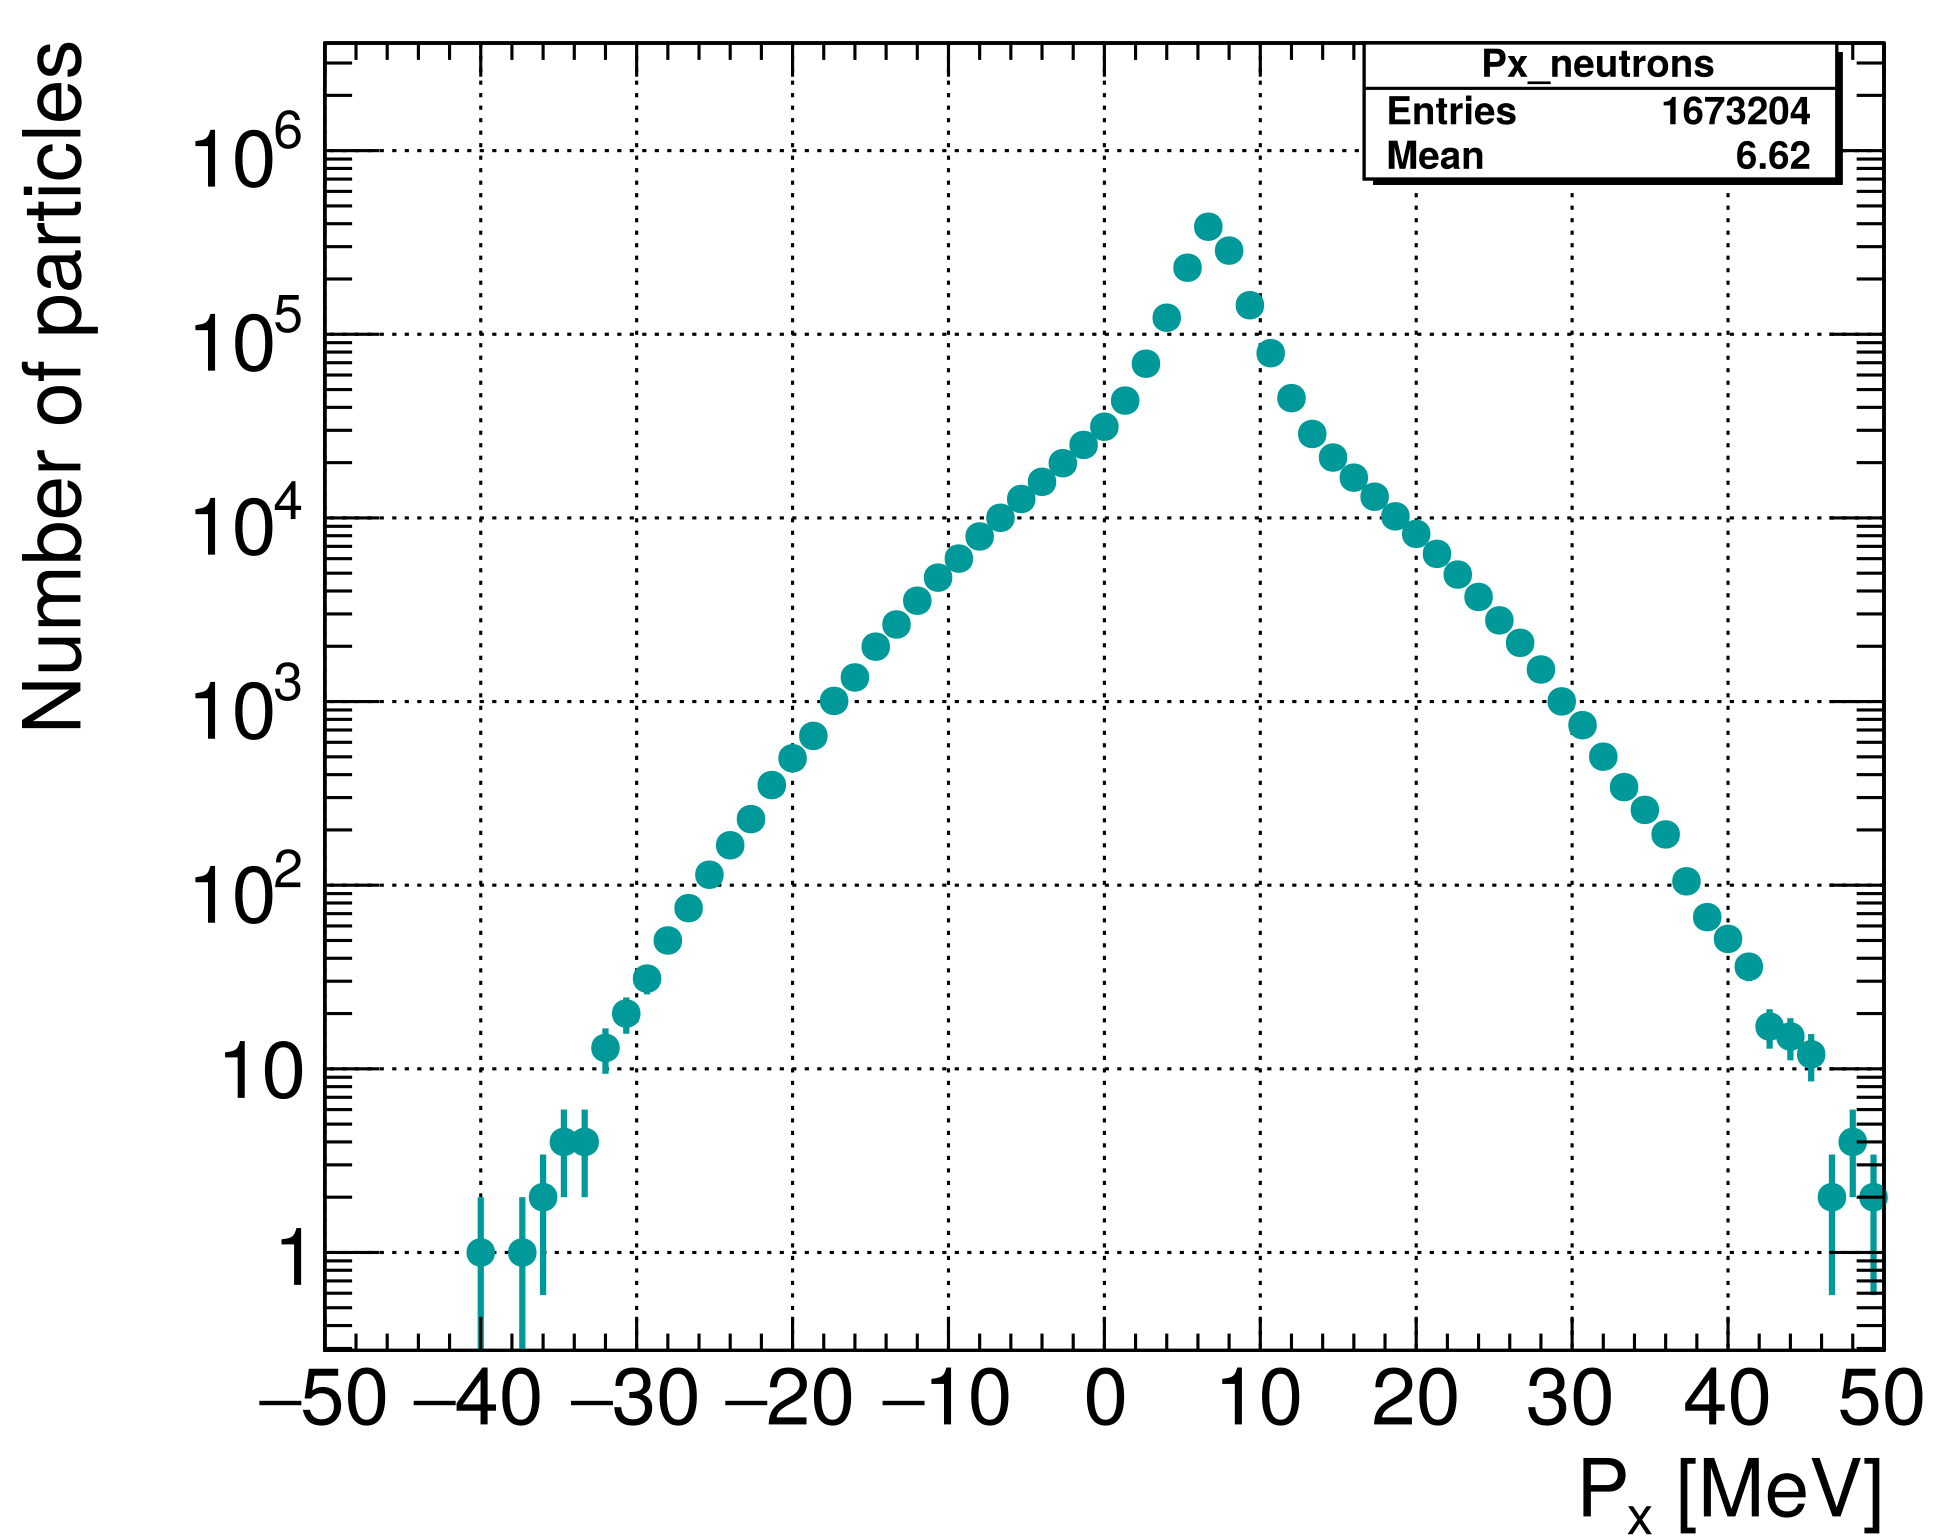
\includegraphics[width=\textwidth]{Figures/BeamDump/neutrons_Px.png}
   \caption{Momentum in x}
   \end{subfigure}
   \hfill
   \begin{subfigure}[b]{0.32\textwidth}
   \centering
    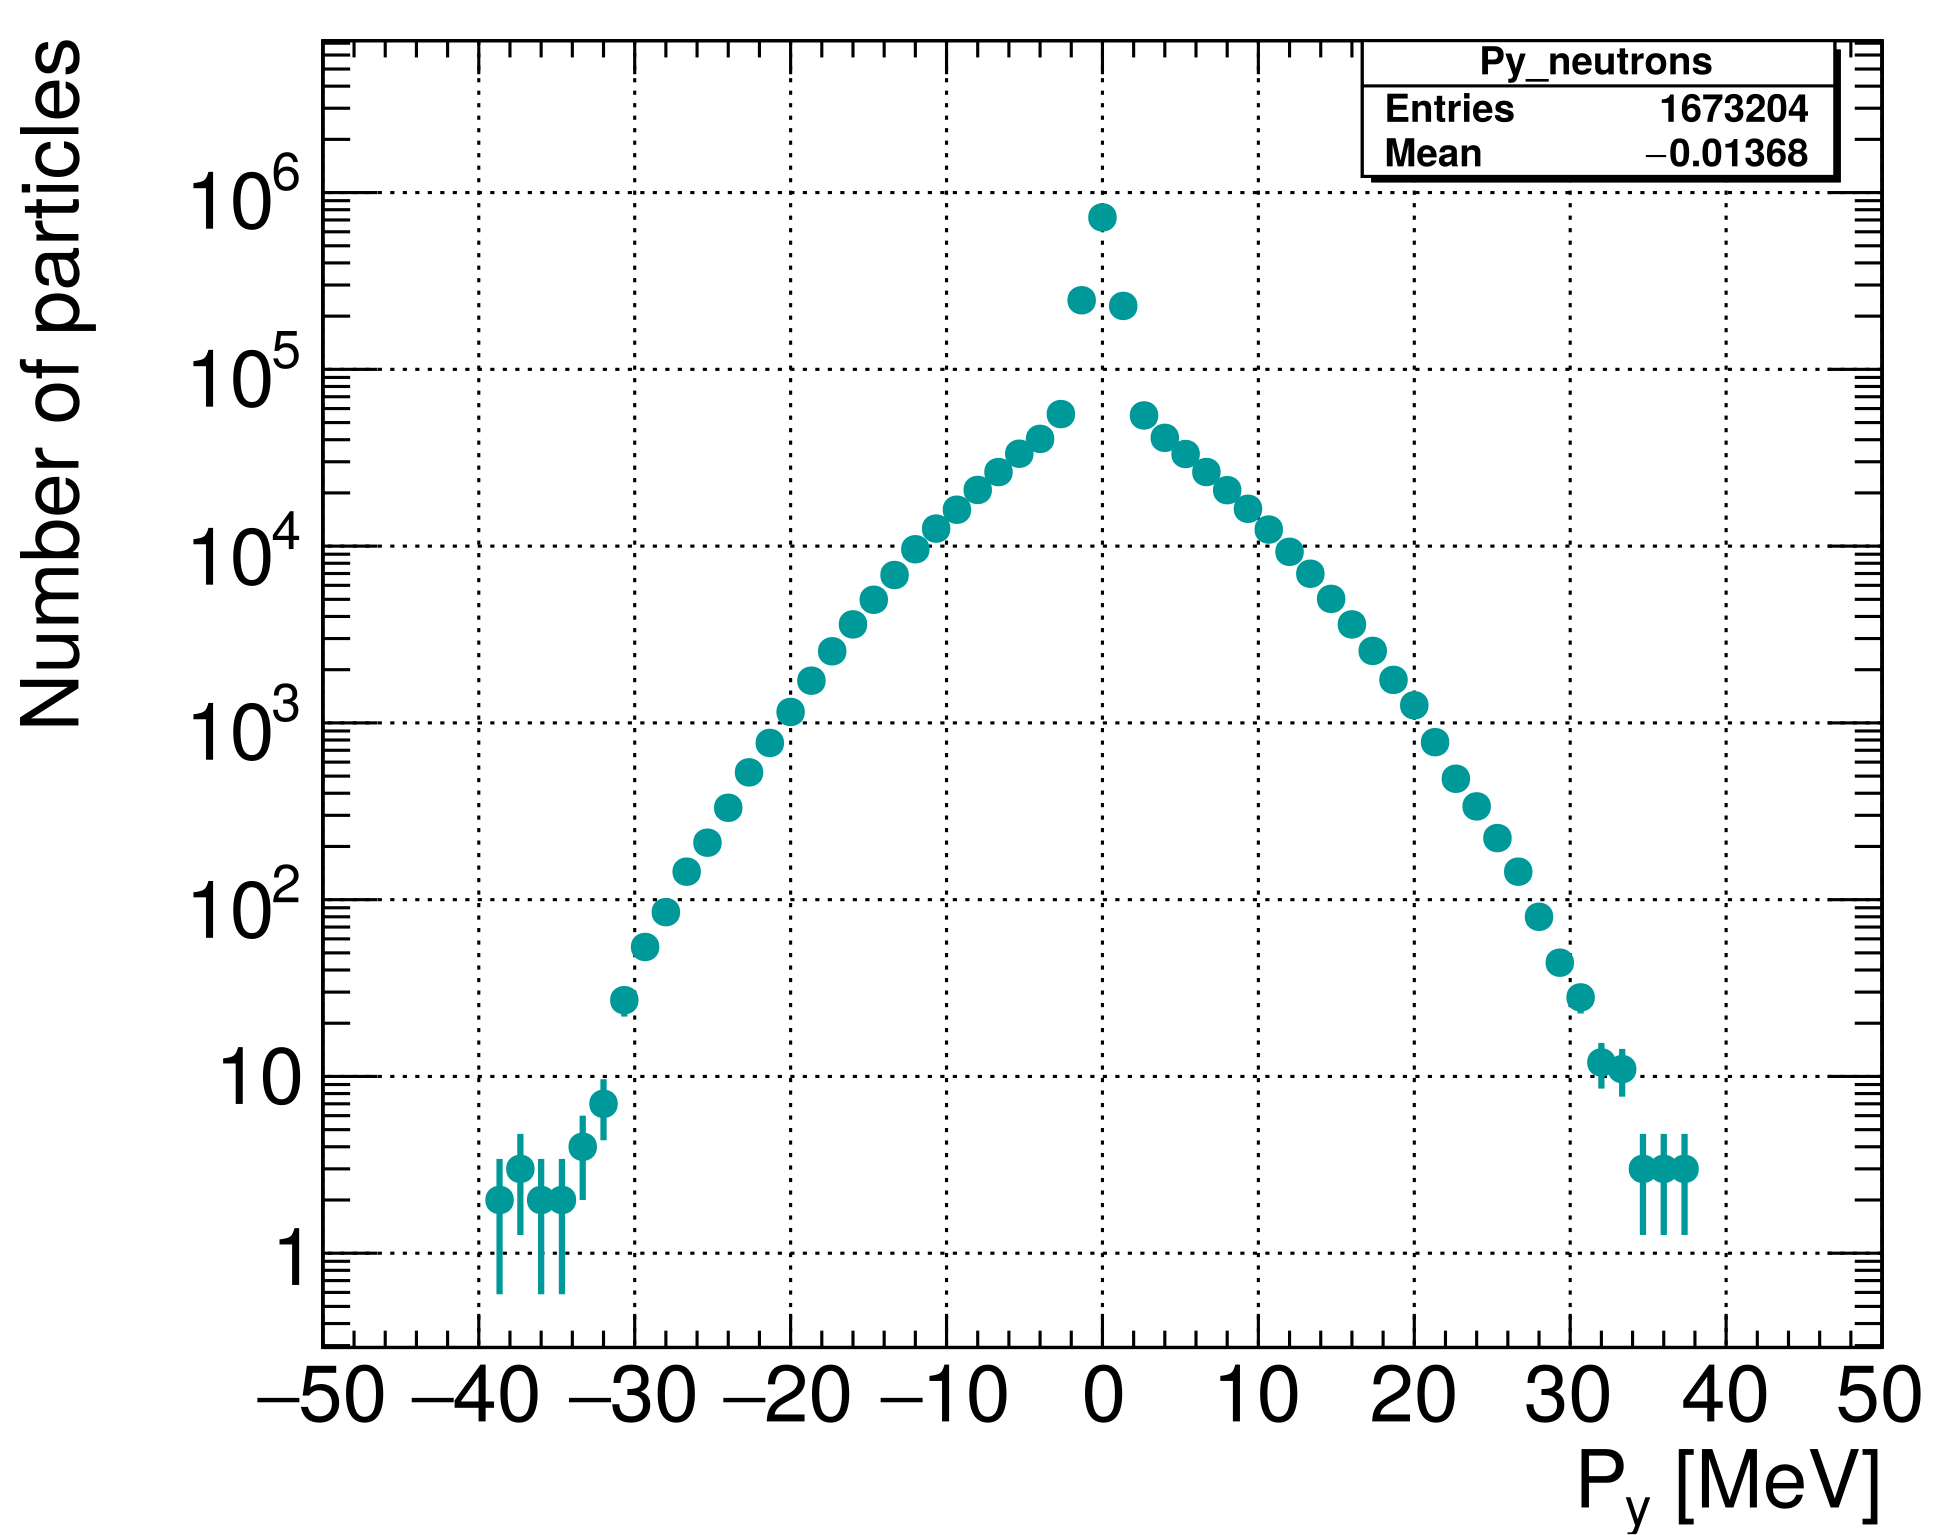
\includegraphics[width=\textwidth]{Figures/BeamDump/neutrons_Py.png}
   \caption{Momentum in y}
   \end{subfigure}
   \hfill
    \begin{subfigure}[b]{0.32\textwidth}
   \centering
    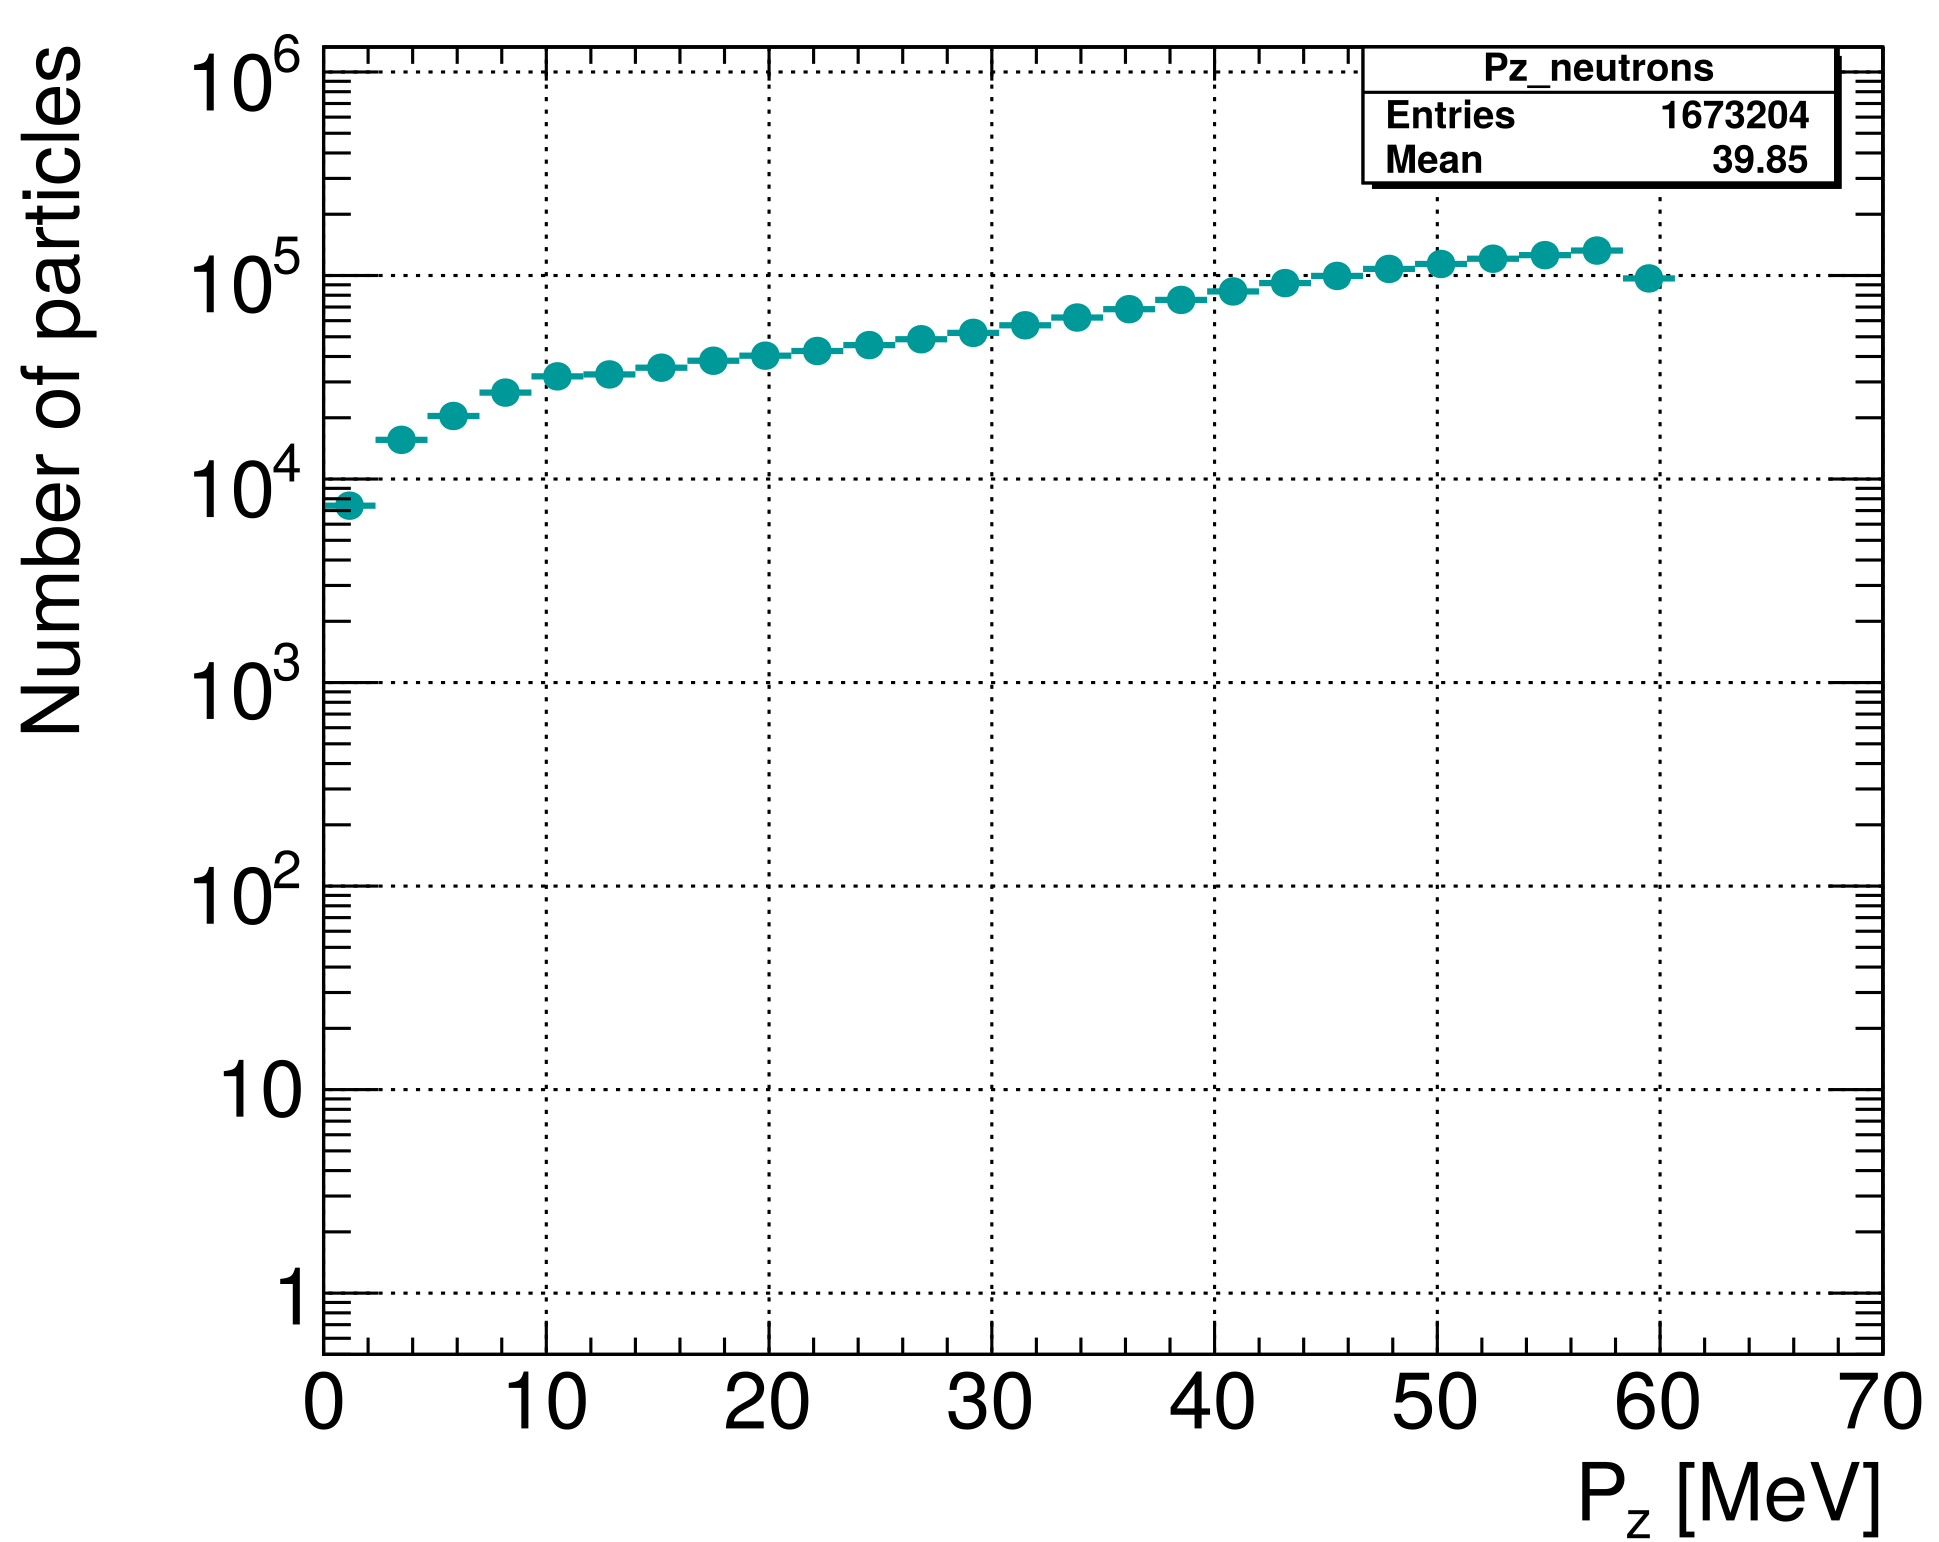
\includegraphics[width=\textwidth]{Figures/BeamDump/neutrons_Pz.png}
   \caption{Momentum in z}
   \end{subfigure}
   \caption[Beam dump neutron momenta in \sid]{Momentum distribution of neutrons in \sid, which originate from one extraction line side.
   The momentum distributions in x, y, and z are given in Figures (a), (b), and (c) respectively.}
   \label{fig:BeamDumps:NeutronMom}
\end{figure} 
The distribution for P\textsubscript{y} is symmetric around 0, P\textsubscript{x} is however shifted to positive values.
This is due to the geometry of the extraction line tunnel and the neutron spatial distribution at the exit of the tunnel.
The neutrons originate in the beam dump hall around the beam pipe axis, i.e. around (0,0) in the xy-plane.
Due to the shape of the extraction tunnel, neutrons with momenta directed in the negative x-direction are absorbed by the tunnel wall along the extraction line.
Additionally, the extraction line components shield the neutron flux around the beam line axis, cutting away further neutrons that are pointed in the negative x-direction.
Since the beam line axis is vertically in the center of the tunnel, which reaches from \SI{-2}{\meter} to \SI{2}{\meter}, the y-distribution of the neutron momenta is symmetrical around \SI{0}{\MeV}.
\\The P\textsubscript{z} distribution reaches from 0 to \SI{60}{\MeV}, with more particles at higher energies.
The low P\textsubscript{z} neutrons have missed the detector or have been absorbed in the non-active calorimeter layers and the Pacman shielding (see Section~\ref{ILC:SiD}).

\begin{figure}[!b]
 \centering
  \begin{subfigure}[b]{0.46\textwidth}
   \centering
    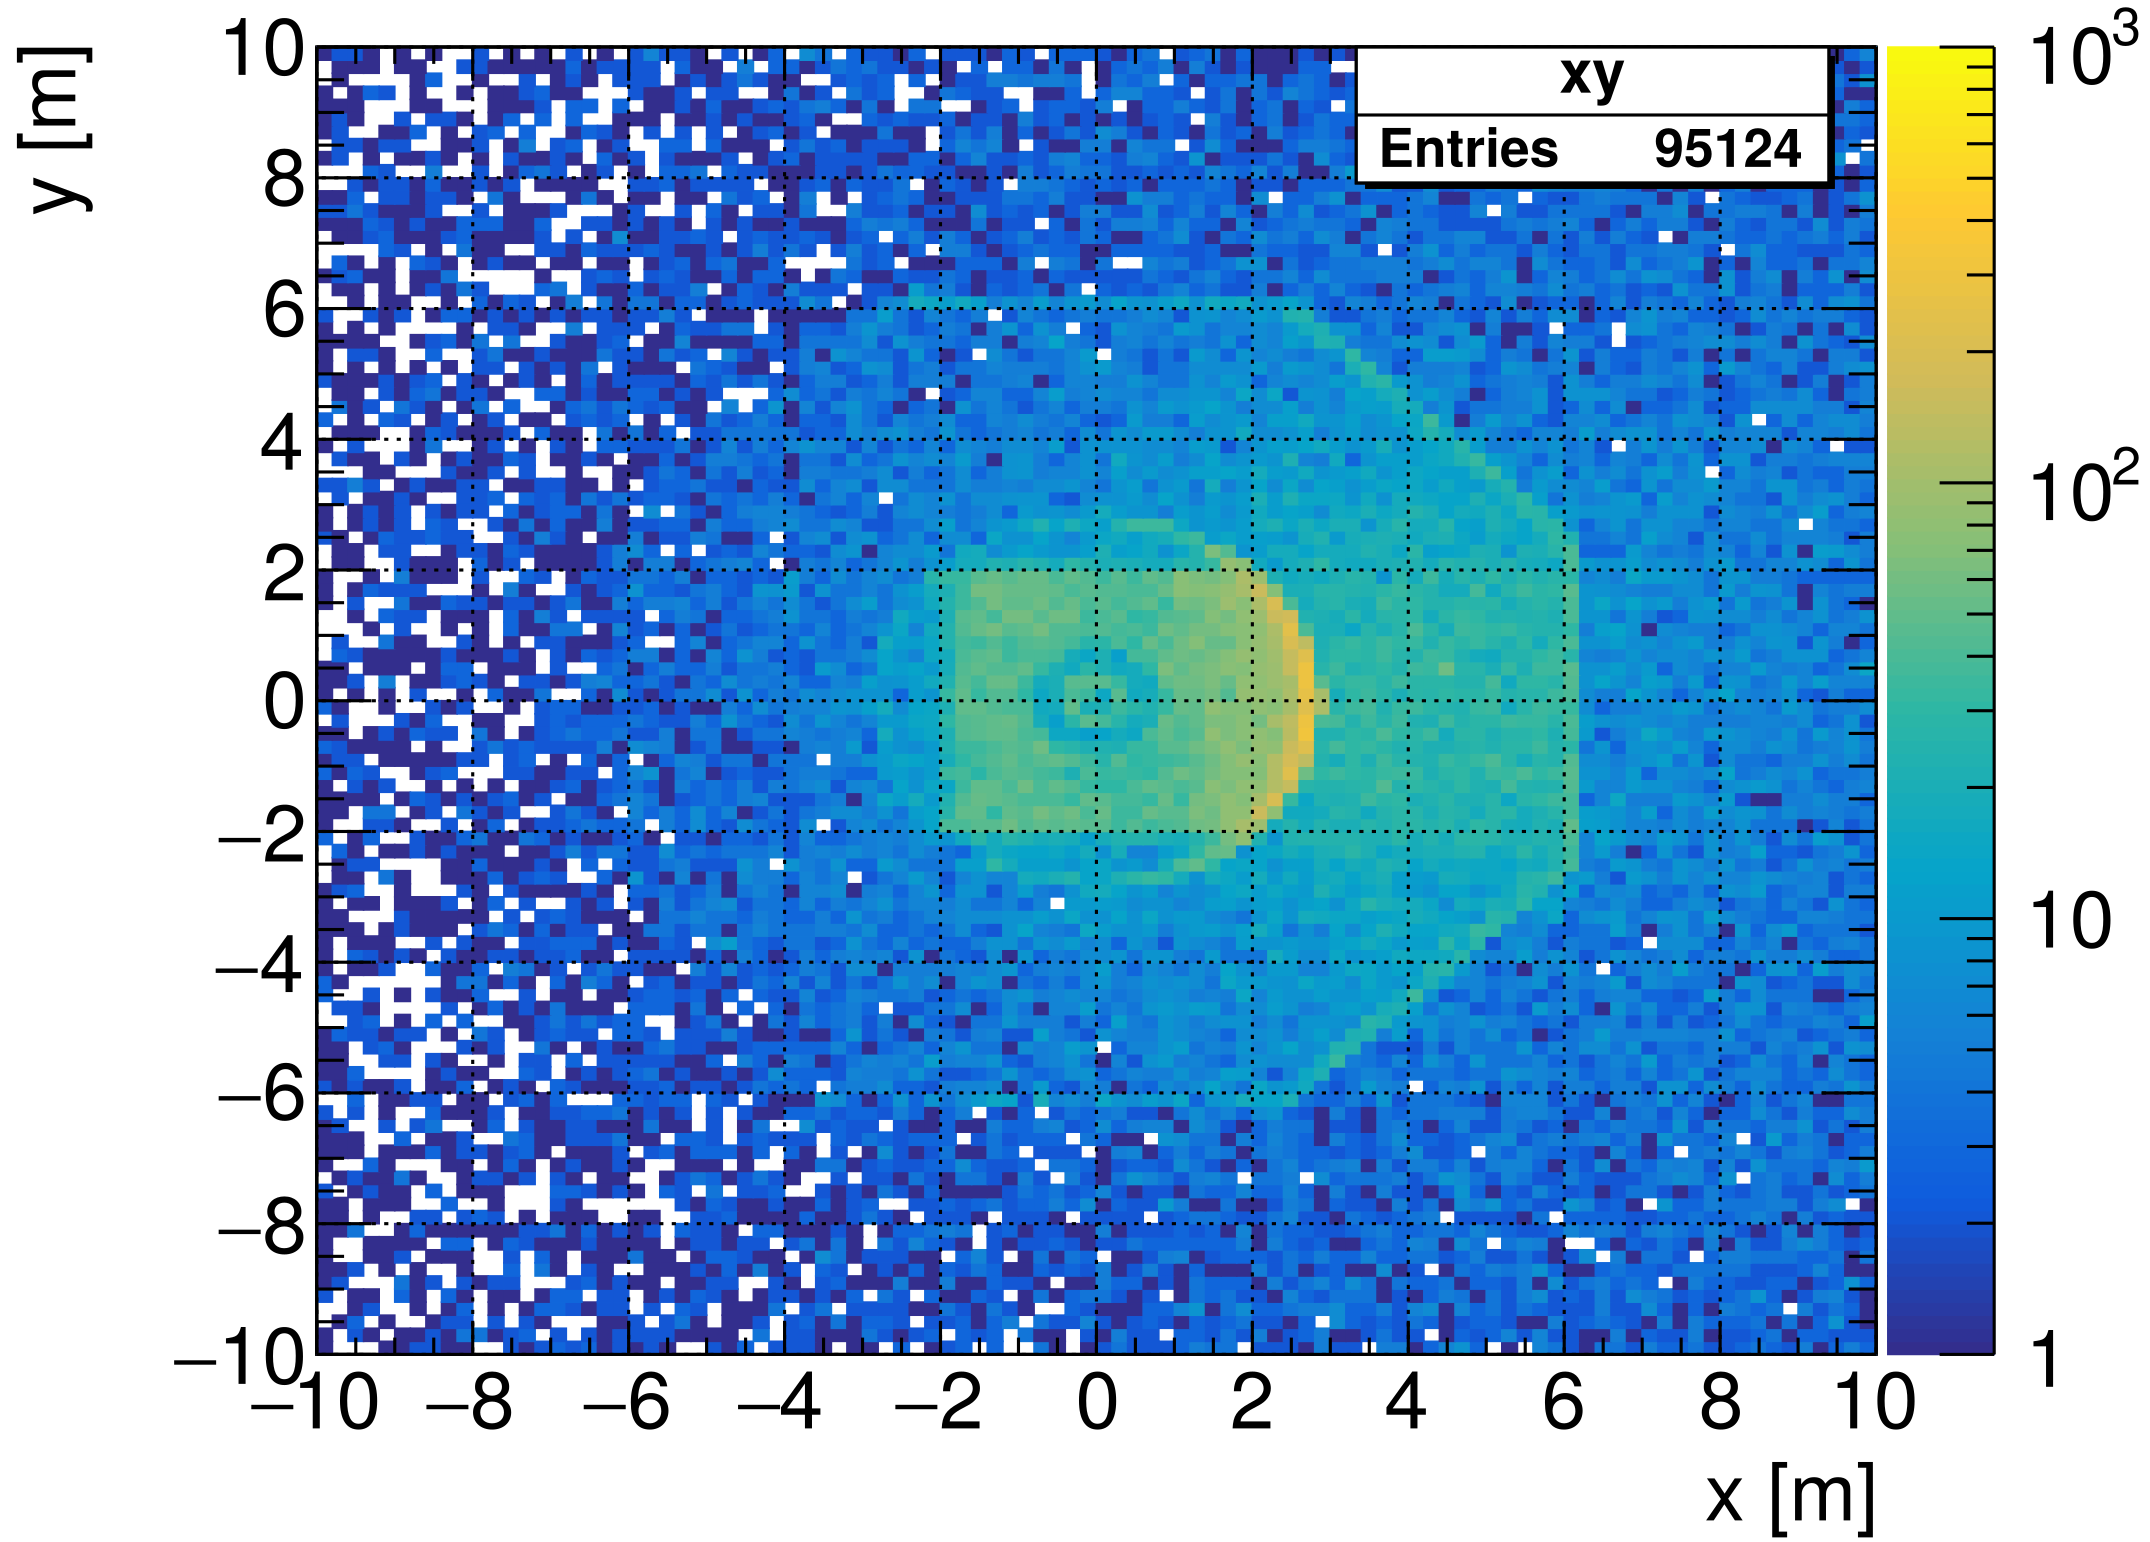
\includegraphics[width=\textwidth]{Figures/BeamDump/neutrons_EndpointMap_xy.png}
   \caption{xy-view}
   \end{subfigure}
   \hfill
   \begin{subfigure}[b]{0.46\textwidth}
   \centering
    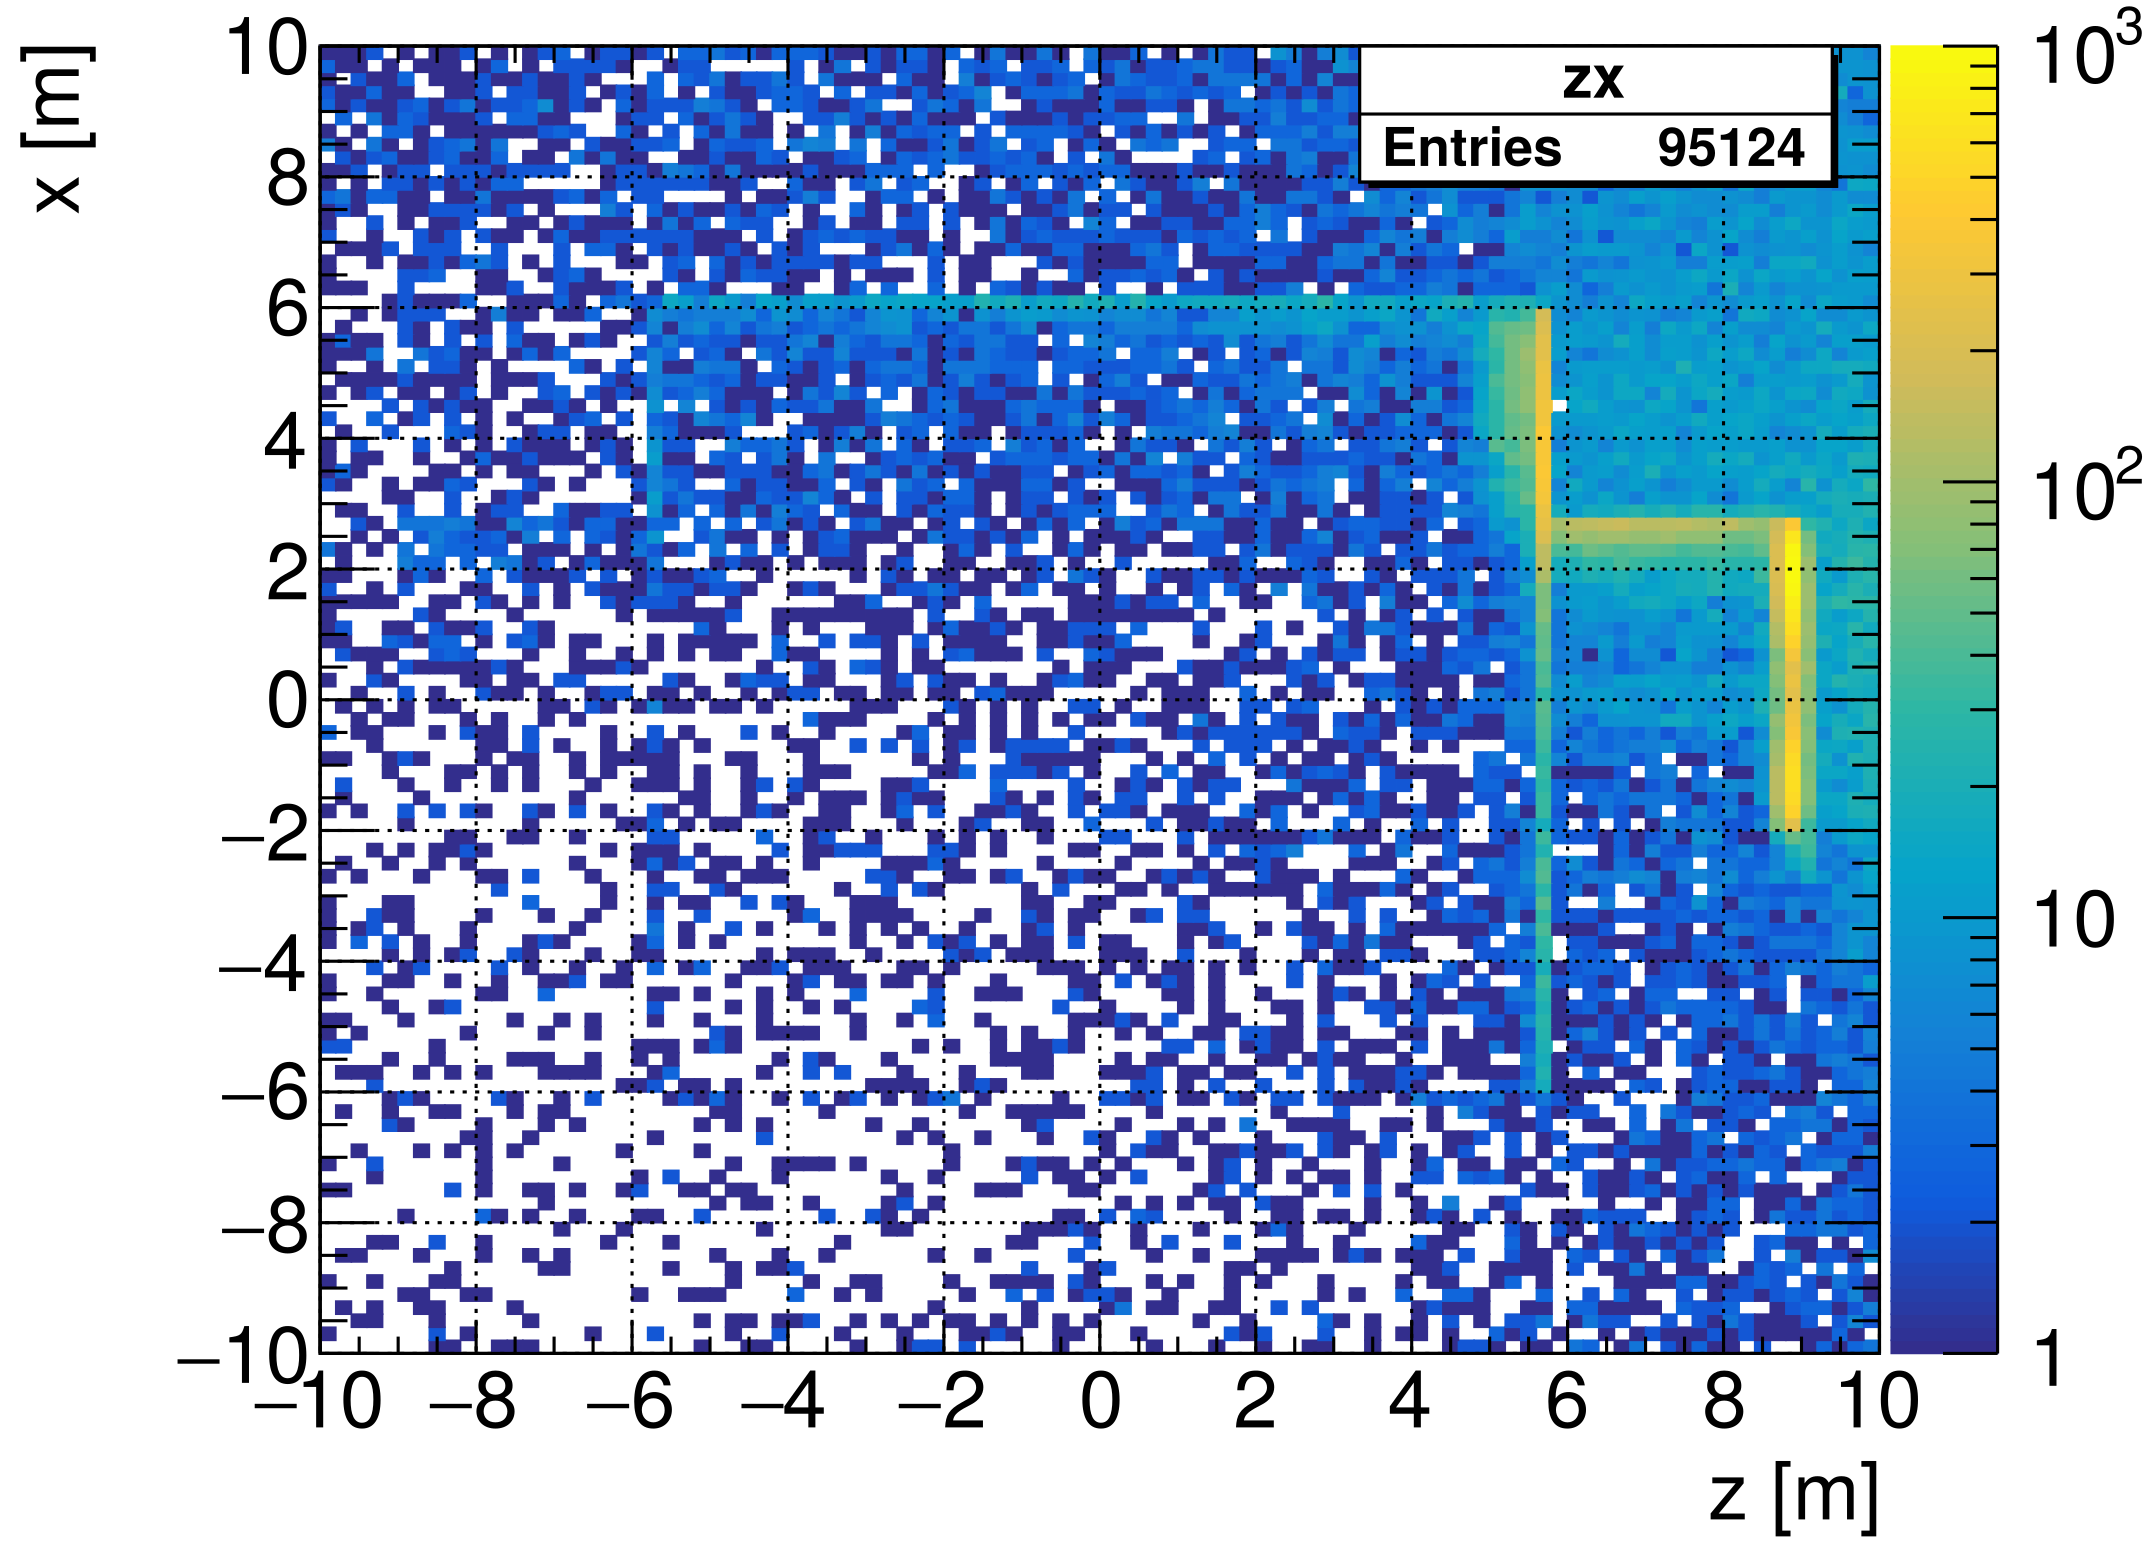
\includegraphics[width=\textwidth]{Figures/BeamDump/neutrons_EndpointMap_zx.png}
   \caption{zx-view}
   \end{subfigure}\\
    \begin{subfigure}[b]{0.46\textwidth}
   \centering
    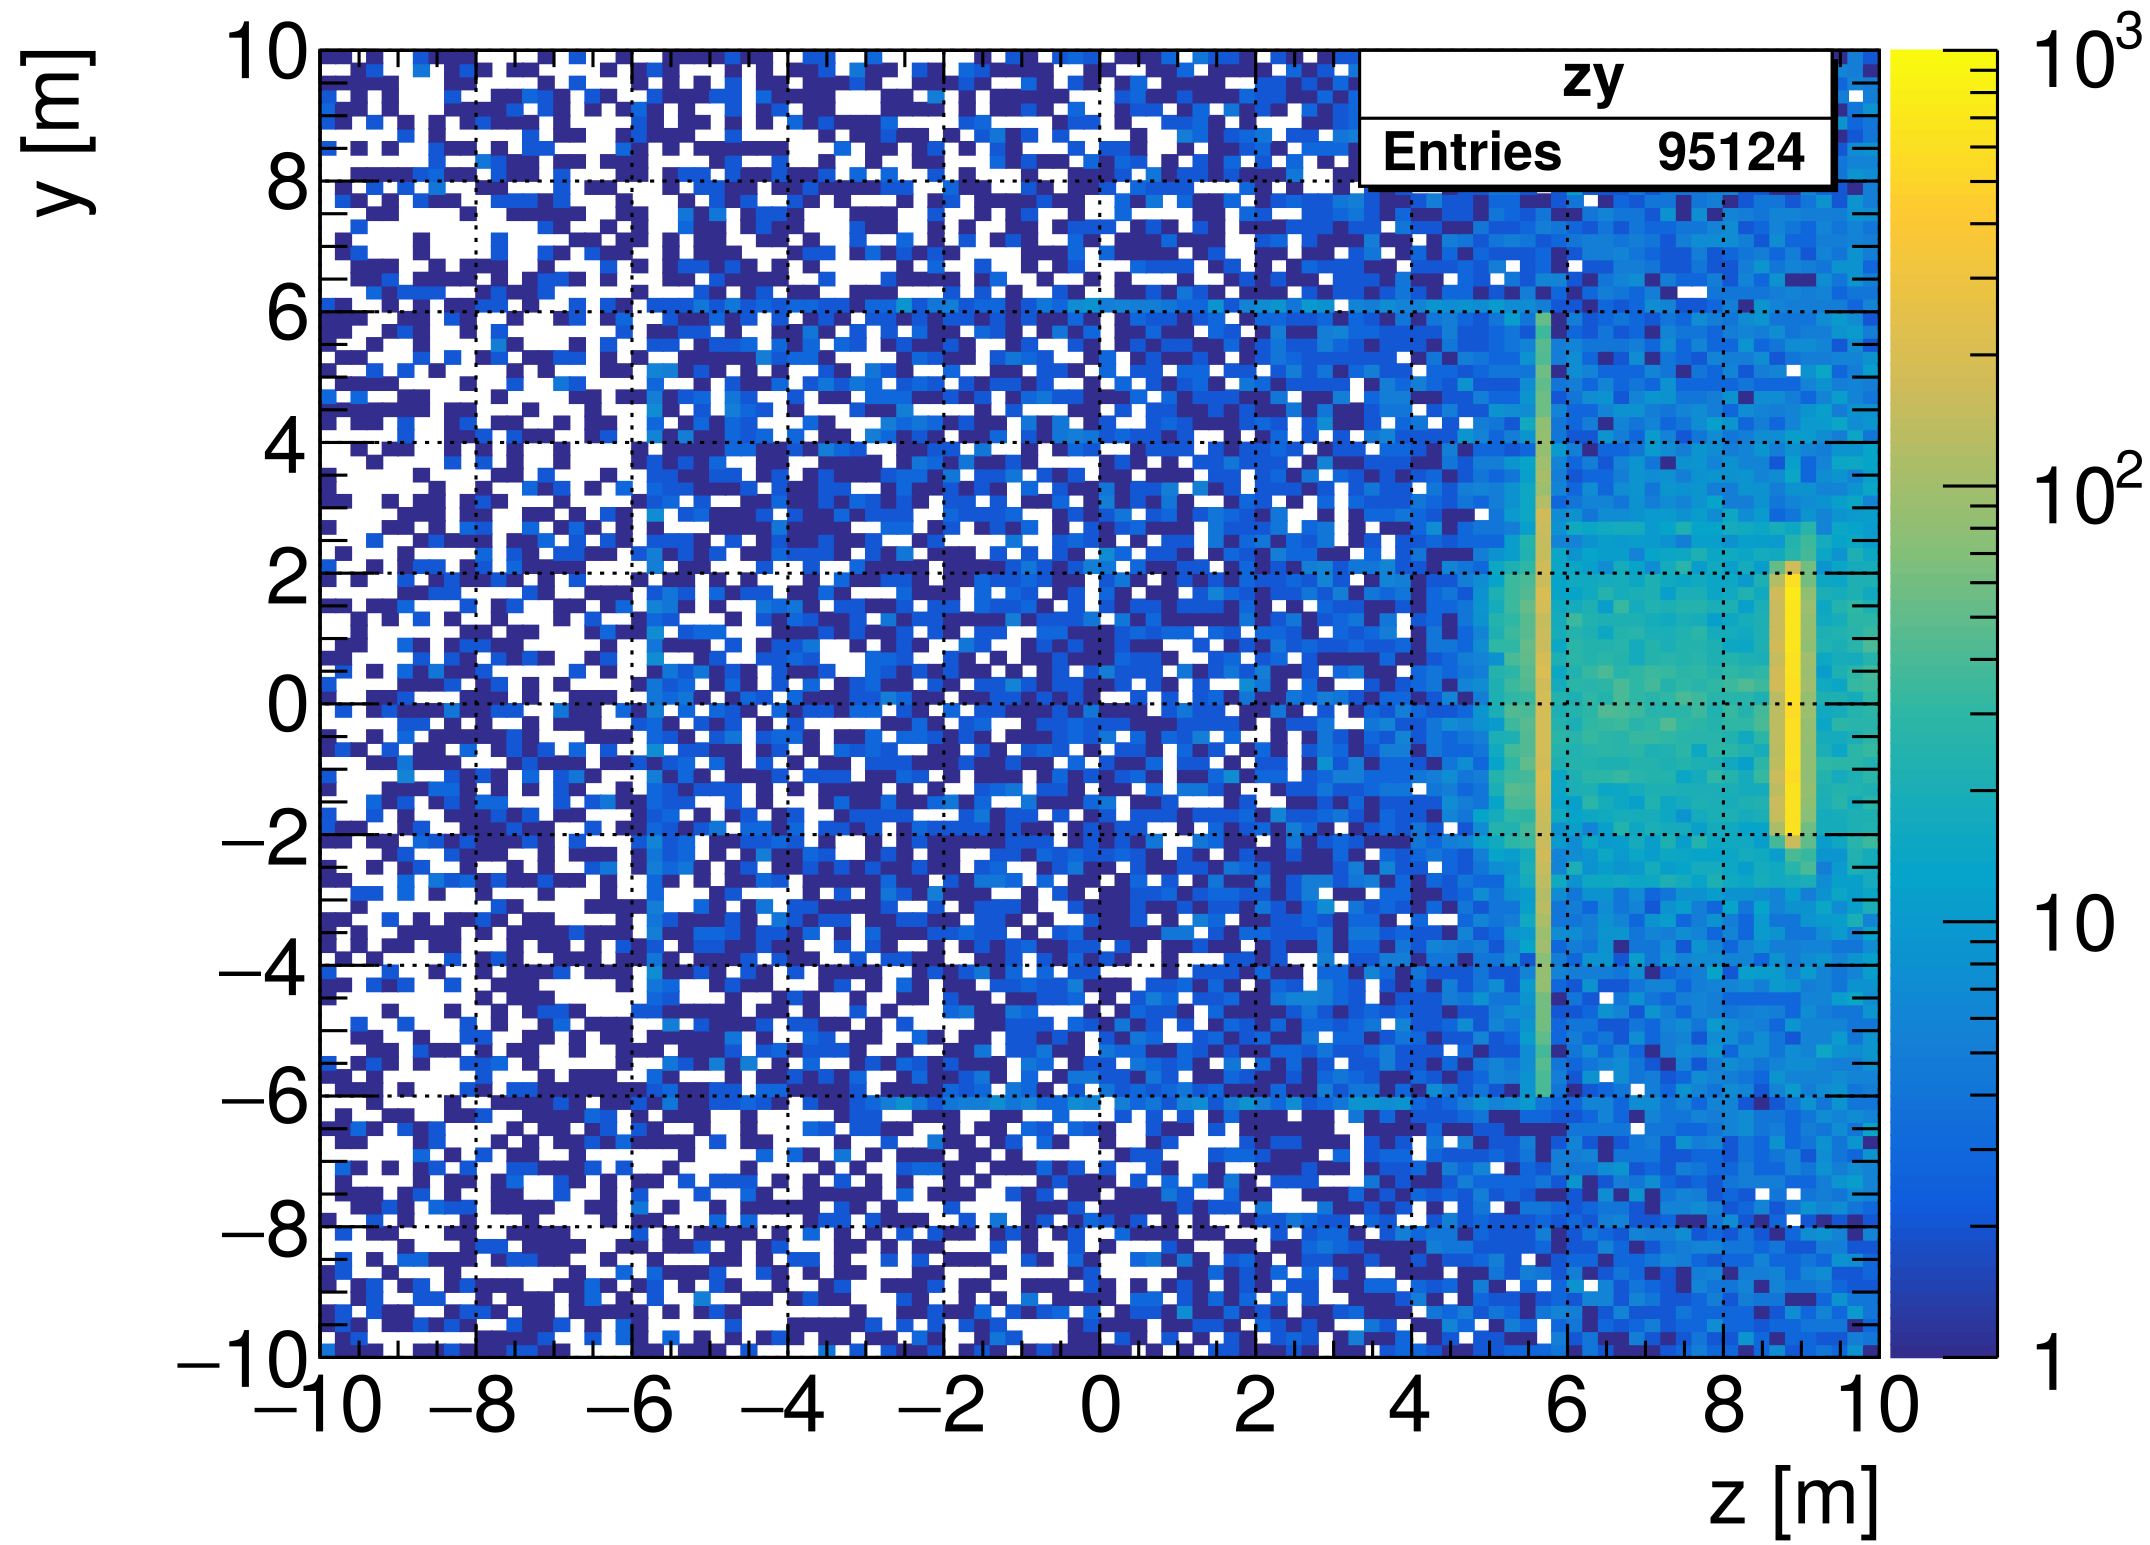
\includegraphics[width=\textwidth]{Figures/BeamDump/neutrons_EndpointMap_zy.png}
   \caption{zy-view}
   \end{subfigure}
   \hfill
   \begin{minipage}{0.45\textwidth}
   \hfill
    \end{minipage}
   \caption[Beam dump neutrons absorbed without leaving hit in \sid]{Maps of the positions in the simulated geometry model, where the beam dump neutrons that have not left any hits in \sid have been absorbed.
   The views of the xy-plane, zx-plane, and zy-plane are given in Figures (a), (b), and (c) respectively.
   The color scale shows the number of neutron endpoint positions per \SI[detect-all]{20}{\centi\meter}$\times$\SI[detect-all]{20}{\centi\meter}.}
   \label{fig:BeamDumps:NeutronMissedMaps}
\end{figure} 
\FloatBarrier
Figure~\ref{fig:BeamDumps:NeutronMissedMaps} shows the positions in the xy-, zx-, and zy-plane, where neutrons that have not left hits in the \sid detector have been absorbed.
The Pacman shielding, which is located behind the endcaps of the \sid muon system (stretching in z from about \SI{5.8}{\meter} to \SI{9.2}{\meter} from the IP), is clearly visible in all three Figures~\ref{fig:BeamDumps:NeutronMissedMaps} (a), (b), and (c).
Here, up to \num{e3} neutrons per unit area are absorbed in the boronated concrete of the Pacman shielding.
But also in the outermost non-active layers of the \sid muon system a significant amount of neutrons are stopped.

\begin{figure}[!b]
 \centering
  \begin{subfigure}[b]{0.4\textwidth}
   \centering
    \includegraphics[width=\textwidth]{Figures/BeamDump/Event_display_neutrons_in_SiD_xy_inverted.png}
   \caption{xy-view}
   \end{subfigure}
   \hfill
   \begin{subfigure}[b]{0.4\textwidth}
   \centering
    \includegraphics[width=\textwidth]{Figures/BeamDump/Event_display_neutrons_in_SiD_xz_inverted_Label.png}
   \caption{zx-view}
   \end{subfigure}\\
    \begin{subfigure}[b]{0.4\textwidth}
   \centering
    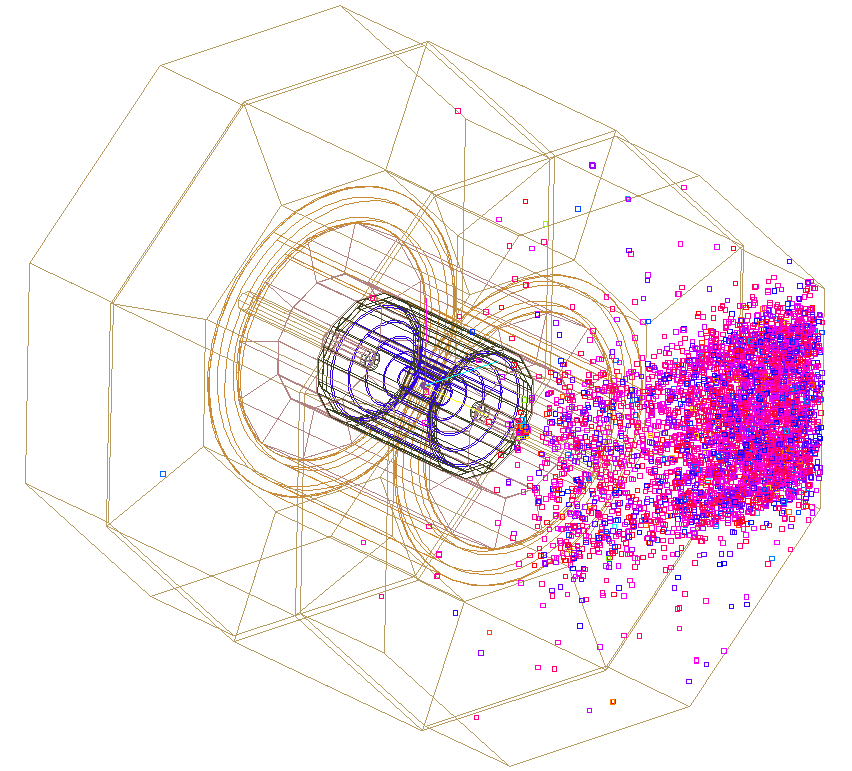
\includegraphics[width=\textwidth]{Figures/BeamDump/Event_display_neutrons_in_SiD_3D_inverted.png}
   \caption{3D-view}
   \end{subfigure}
   \caption[Event displays of the beam dump neutron hits in \sid]{Event displays created with WIRED4 of the \sid hits from ILC beam dump neutrons.
   The views of the xy-plane, zx-plane, and a 3D-view are given in Figures (a), (b), and (c) respectively.}
   \label{fig:BeamDumps:NeutronEventDisplays}
\end{figure} 
\FloatBarrier
\newpage
The spatial distributions of the neutrons, which hit the active layers of the \sid detector, are best seen in an event display of the \sid detector.
Figure~\ref{fig:BeamDumps:NeutronEventDisplays} shows the WIRED4 event displays in various views.
The hits are mainly restricted to the outer layers of the muon system.
Their spatial distribution is determined by the shape of the extraction line tunnel.
In Figure~\ref{fig:BeamDumps:NeutronEventDisplays} (b), hits in the \sid BeamCal are also visible.

From one ILC bunch dumped in the main beam dump, the number of hits in the \sid subdetectors from the resulting neutrons from one of the extraction line tunnels are given in a bar chart in Figure~\ref{fig:BeamDumps:HitsPerSubdetector}.
As already expected from the event displays in Figure~\ref{fig:BeamDumps:NeutronEventDisplays}, the \sid muon endcaps get the most hits with about \num{1.5e4}.
About two orders of magnitude fewer hits are counted in the muon barrel and the BeamCal.
Also the LumiCal subdetector is hit about \num{20} times by neutrons from one beam dump.
All other inner \sid subdetectors are shielded by the outer subdetectors and the Pacman shielding, and are not hit.
\\Figure~\ref{fig:BeamDumps:HitTime} shows the time of the hits in the \sid muon system and the BeamCal with respect to the time of their creation, which is the time of the ILC beam being dumped in the main beam dump.
Due to its high energy, the time of the beam arriving at the main beam dump can be approximated as the time of the bunch crossing.
Using this approximation, the neutrons arrive at the \sid detector up to \SI{100}{\micro\second} after the bunch crossing.
Since every bunch is separated by \SI{554}{\nano\second} (see Section~\ref{ILC:SiD:readout}), the neutrons coincide with the next 180 ILC bunches.
\begin{figure}[!h]
\centering
\begin{minipage}[t]{0.49\textwidth}
\centering
 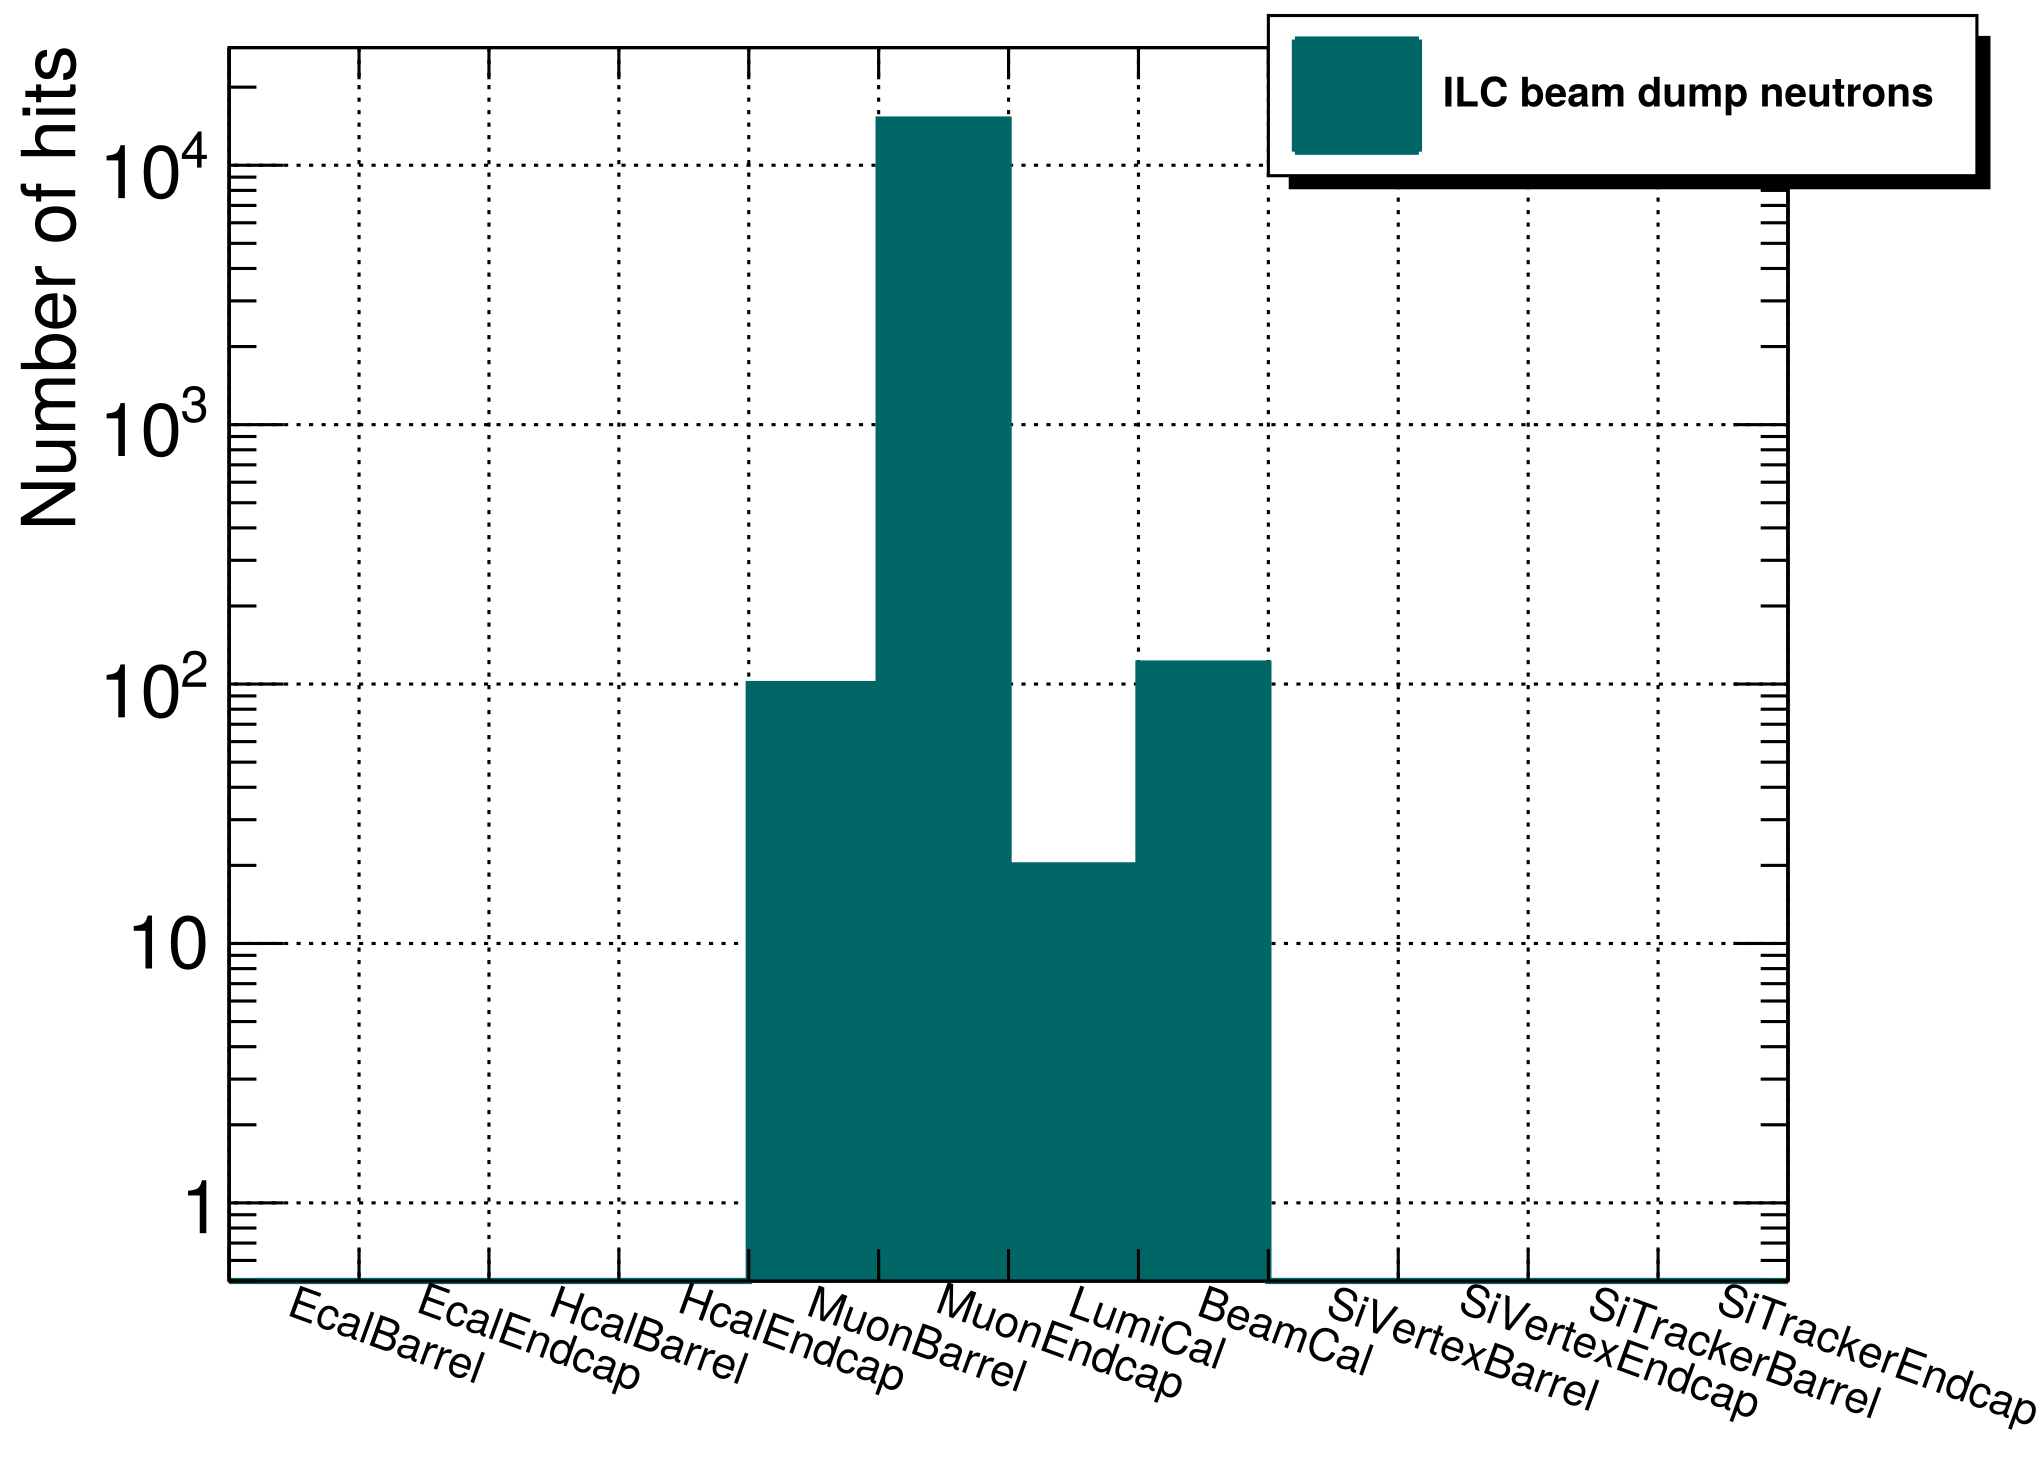
\includegraphics[width=\textwidth]{Figures/BeamDump/Hits_in_SiD_subdetectors.png}
\caption[Number of hits in the \sid subdetectors of the ILC main beam dump neutrons]{Bar chart of the number of hits in the individual \sid subdetector from neutrons coming from one ILC main beam dump, after a beam bunch has been dumped.}
\label{fig:BeamDumps:HitsPerSubdetector}
\end{minipage}
\hfill
\begin{minipage}[t]{0.49\textwidth}
\centering
 \includegraphics[width=\textwidth]{Figures/BeamDump/neutrons_hittime.pdf}
\caption[Neutron hit time in the \sid subdetectors]{Hit time distribution in the \sid subdetectors that are hit by neutrons coming from one ILC main beam dump, after a beam bunch has been dumped.}
\label{fig:BeamDumps:HitTime}
\end{minipage}
\end{figure}
\\By counting the number of hits per cell in the BeamCal and the muon barrel and endcaps, the number of dead cells is calculated for the assumed buffer depths in the subdetectors.
This was done in the same way as described in Sections~\ref{PairBkg:occupancy} and~\ref{BDS_Muons:sidocc}.
A cell is called ``dead'', when all its buffers are filled and no further hits can be stored.
Figure~\ref{fig:BeamDumps:NeutronOcc} shows the fraction of dead cells as a function of the assumed buffer depth in the \sid muon system and the \sid BeamCal.
Since the muon endcaps collect the most neutron hits, the fraction of dead cells were calculated for up to a buffer depth of five.
In the muon barrel, however, all hit cells are hit only one time, because of which only the first bin is filled in this plot (Figure~\ref{fig:BeamDumps:NeutronOcc} (a)).
Similarly for the BeamCal, the cells are hit up to two times.
\\Although these studies are done for neutrons from one ILC bunch only and the occupancy would rise for a bunch-train-worth of neutrons accordingly, the actual number of hits in the scintillating active layers of the muon system would depend on the scintillator material, and the noise threshold of the readout silicon photomultipliers (SiPM).
\\Rather than increasing the detector occupancy, the neutron background will more importantly affect the subdetectors with respect to the radiation damage it causes.
From the presented \geant simulation, it was calculated that the neutron flux for the outermost layer of the muon endcaps is about 530 neutrons \si{\per\meter\squared\per\second}.
For the BeamCal, the flux is about 4 neutrons \si{\per\centi\meter\squared\per\second}.
The expected neutron flux in the BeamCal from secondary photons, which excite giant nuclear dipole resonances~\cite{GDR} and hence cause the emission of neutrons, is considered to be \num{5e13} neutrons \si{\per\centi\meter\squared\per\year}~\cite[p. 134]{TDR4}, which is about \num{1.6e6} neutrons \si{\per\centi\meter\squared\per\second}.
Due to this, the BeamCal will be designed to use radiation hard materials regardless of the additional neutron flux from the main beam dumps.
\begin{figure}[!h]
 \centering
  \begin{subfigure}[b]{0.49\textwidth}
   \centering
    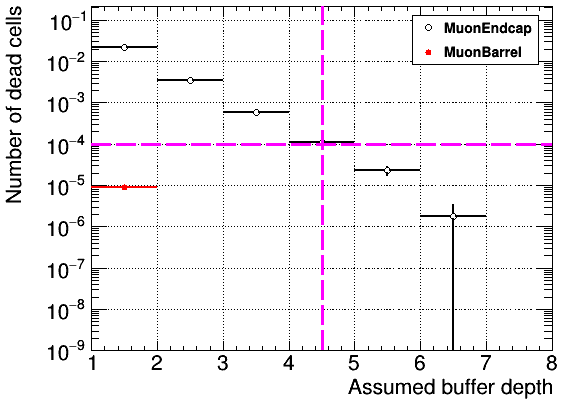
\includegraphics[width=\textwidth]{Figures/BeamDump/Occupancy_Comparison_All_layers_deadcells_BeamDump_Neutrons_MuonSystem.png}
   \caption{\sid muon system}
   \end{subfigure}
   \hfill
   \begin{subfigure}[b]{0.49\textwidth}
   \centering
    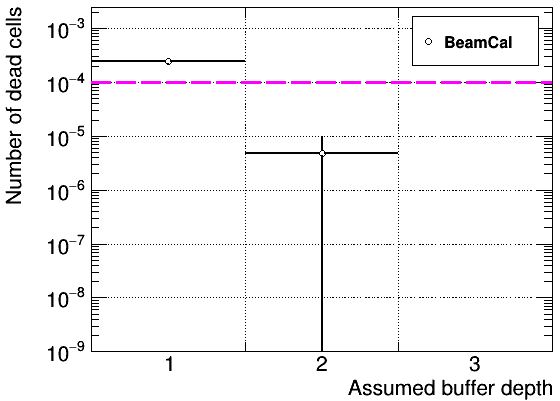
\includegraphics[width=\textwidth]{Figures/BeamDump/Occupancy_Comparison_All_layers_deadcells_BeamDump_Neutrons_BeamCal.png}
   \caption{\sid BeamCal}
   \end{subfigure}
   \caption[Neutron occupancy in the \sid muon system and BeamCal]{Fraction of dead cells in the \sid muon barrel and muon endcap (Figure (a)) and in the \sid BeamCal (Figure (b)) in all layers combined, for neutrons originating form one ILC beam bunch being dumped.
   The fraction is calculated by computing the number of dead cells for a given buffer depth, and normalizing the numbers by the total number of cells in the respective subdetector.
   \\The dashed lines indicate the buffer depth of four for the current sensor design, and the guideline of \num{e-4} for a critical acceptance limit.}
   \label{fig:BeamDumps:NeutronOcc}
\end{figure} 

\section{Alternative beam dump design}
\label{BeamDumps:Alternative}
The current ILC main beam dump designs are based on a water vessel.
The previous sections have shown that due to the high material density, the ILC beam bunches are stopped over a distance of about \SI{12}{\meter}.
This leads to a large energy dissipation in the beam dump and its surroundings.
The resulting high dose rates from the irradiation limits the time the maintenance staff will be allowed to be in the proximity of the beam dumps.
There are, however, other beam dump designs, which do not lead to restricting dose rates of the dumps surroundings.
\\In the following paragraphs, results from a \fluka study are presented concerning the effect of using a gaseous beam dump for the ILC beam.
Such gas dumps have been studied before in the context of the TESLA accelerator~\cite{TESLA_acc, TESLA_beamdump_studies}.
A vessel filled with noble gas requires a dump length of at least \SI{1}{\kilo\meter} in order to dissipate and absorb the beam energy.

\subsection{Deposited energy and irradiation dose}
In the \fluka model of this simple gaseous beam dump, a copper vessel with a length of \SI{1}{\kilo\meter} and a diameter of \SI{150}{\centi\meter} has been assumed.
The vessel has a wall thickness of \SI{55}{\centi\meter}, in order to act as shielding simultaneously, and is filled with nitrogen gas.
Figure~\ref{fig:BeamDumps:GasDump} shows the deposited energy and the resulting instantaneous dose equivalent from one ILC beam bunch, which has the same characteristics as before in Section~\ref{BeamDumps:sim_surrounding}.
From the plots, it becomes apparent that the maximum deposited energy reaches \SI{e8}{\GeV\per\centi\meter\cubed} as well as in the water beam dumps before (see Section~\ref{BeamDumps:sim_surrounding:Energy}).
This is, however, restricted to the back wall of the vessel.
In the surroundings, no observable energy is deposited.
\\The maximum dose equivalent in the gaseous dump is smaller by over one order of magnitude compared to the results for the water vessels (see Section~\ref{BeamDumps:sim_surrounding:Dose}).
Again, the dose is restricted to the gas vessel.
In the direct surroundings, a dose equivalent level of about \SI{e-4}{\milli\sievert\per\centi\meter\cubed} is reached, which is a difference of two to three orders of magnitude compared to the water beam dump.
\begin{figure}[!h]
 \centering
  \begin{subfigure}[b]{0.49\textwidth}
   \centering
    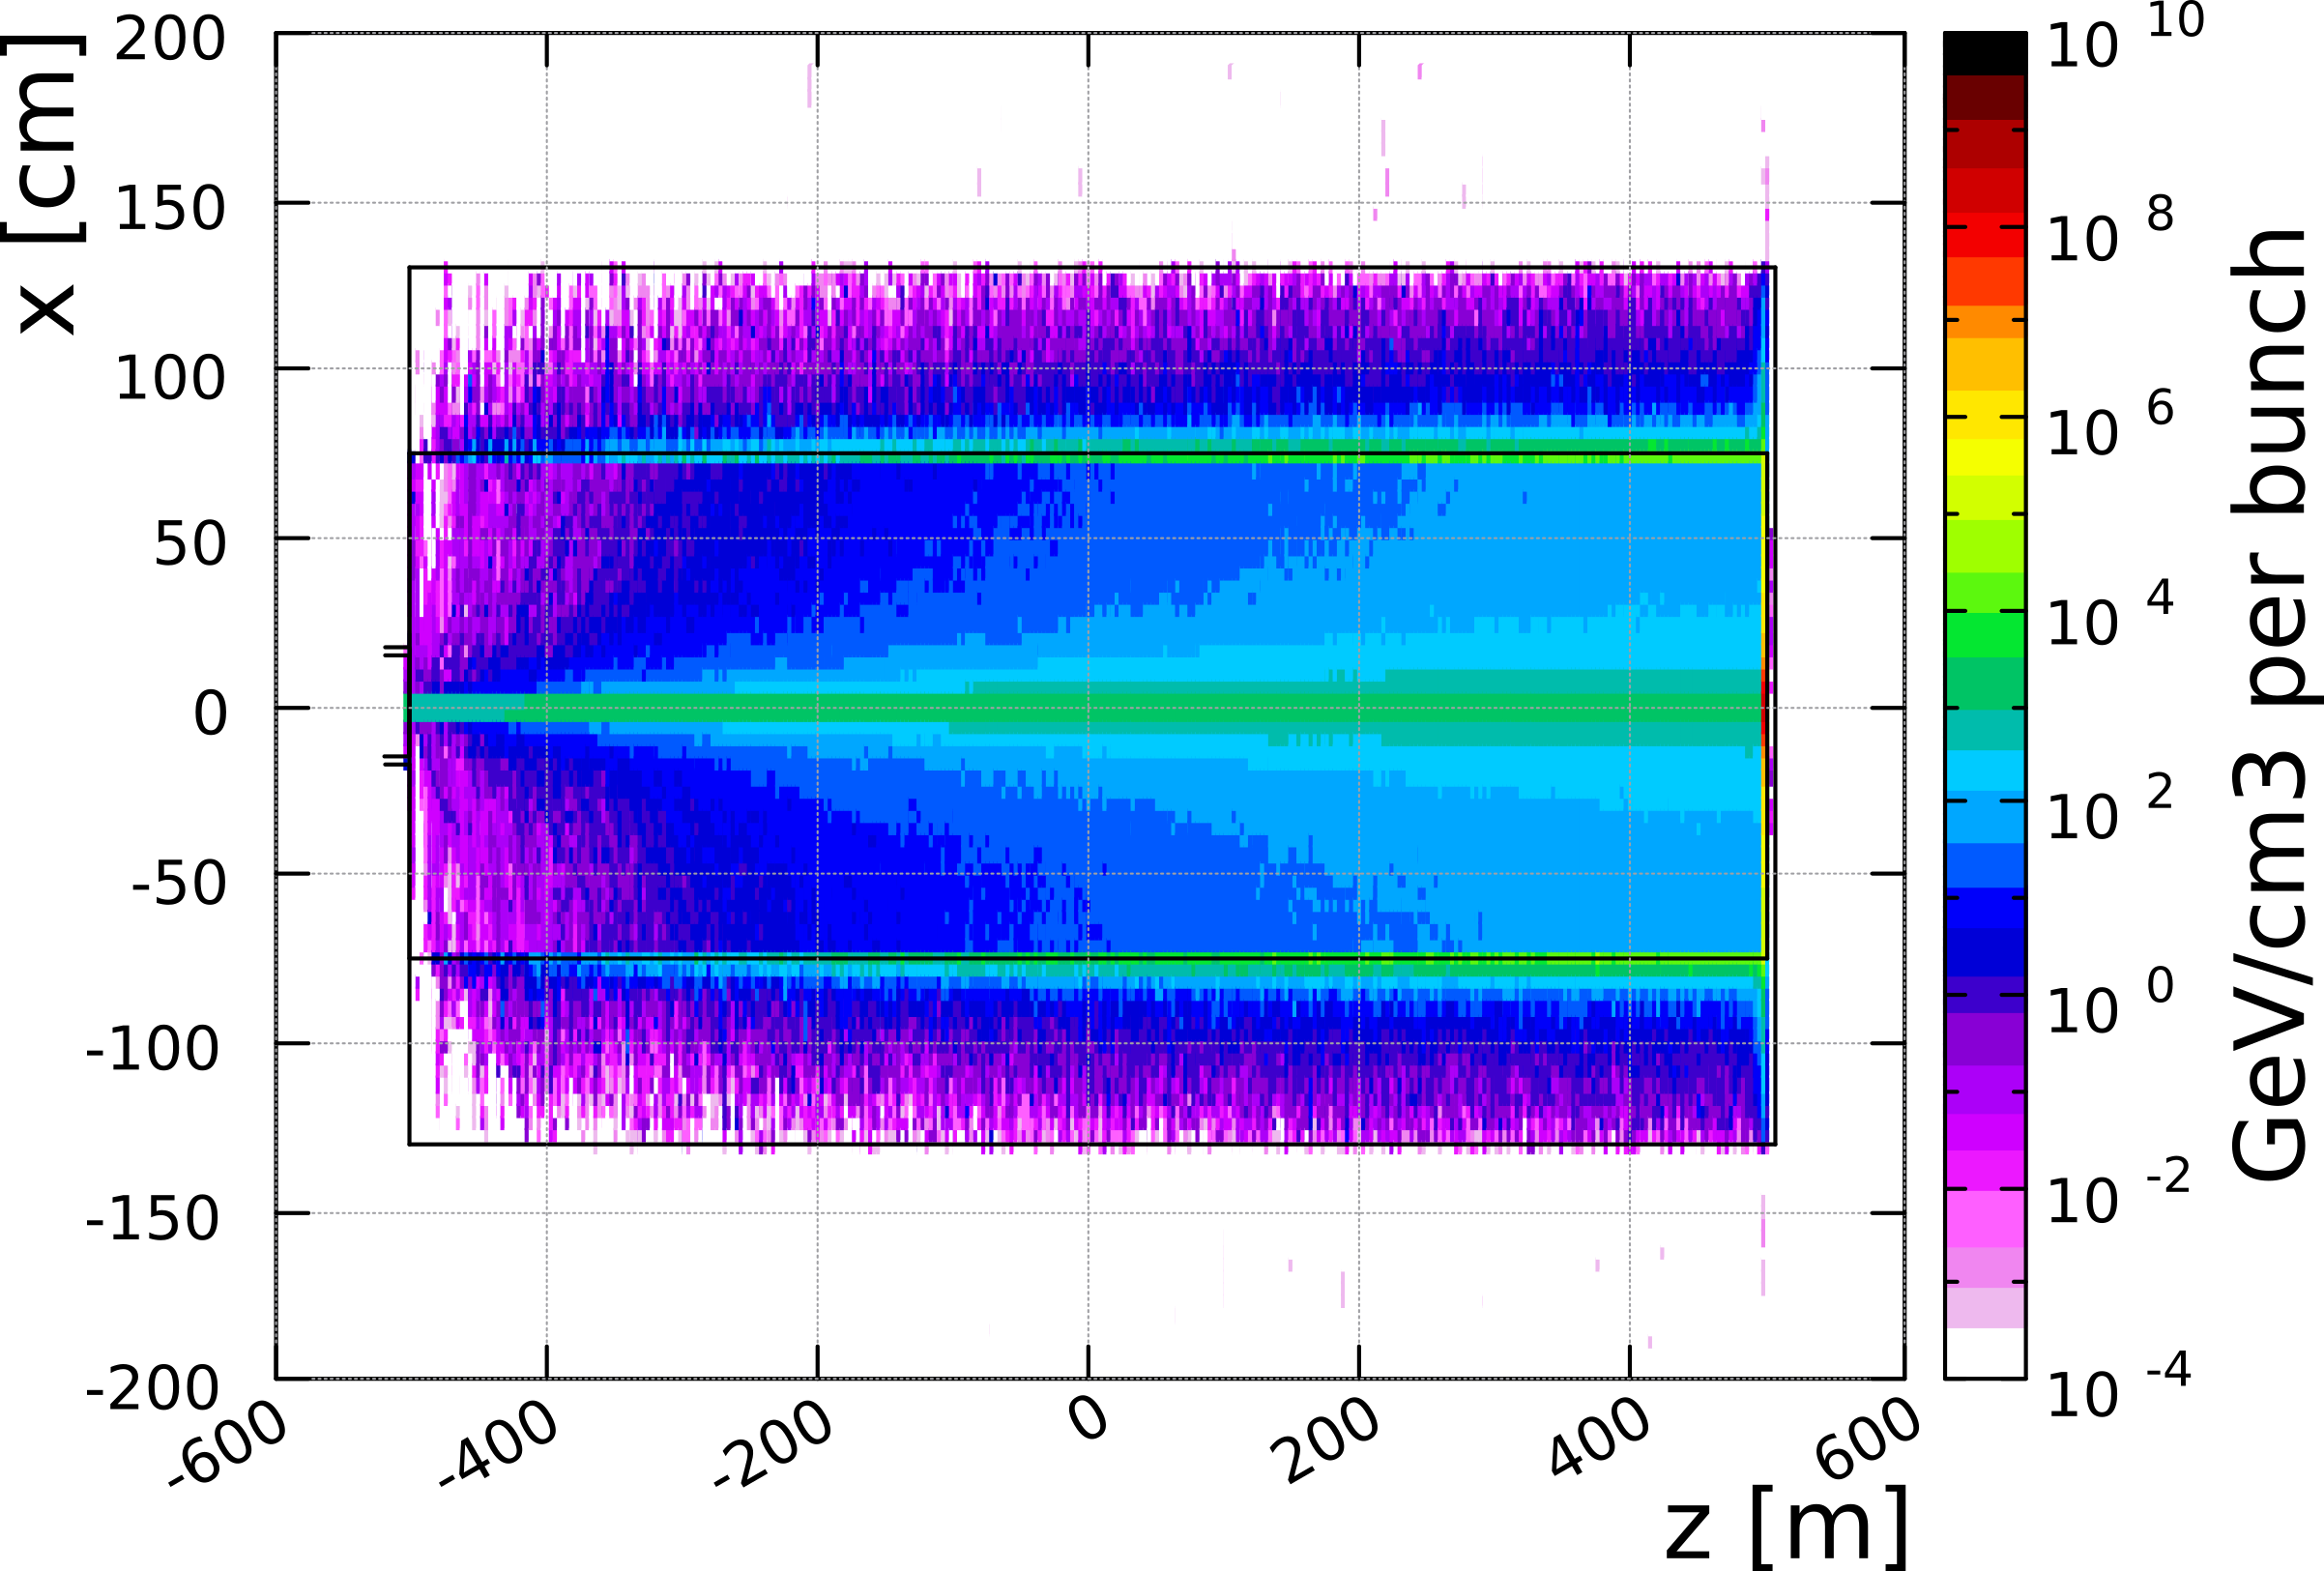
\includegraphics[width=\textwidth]{Figures/BeamDump/Gasdump/Energy.png}
   \caption{Deposited energy}
   \end{subfigure}
   \hfill
   \begin{subfigure}[b]{0.49\textwidth}
   \centering
    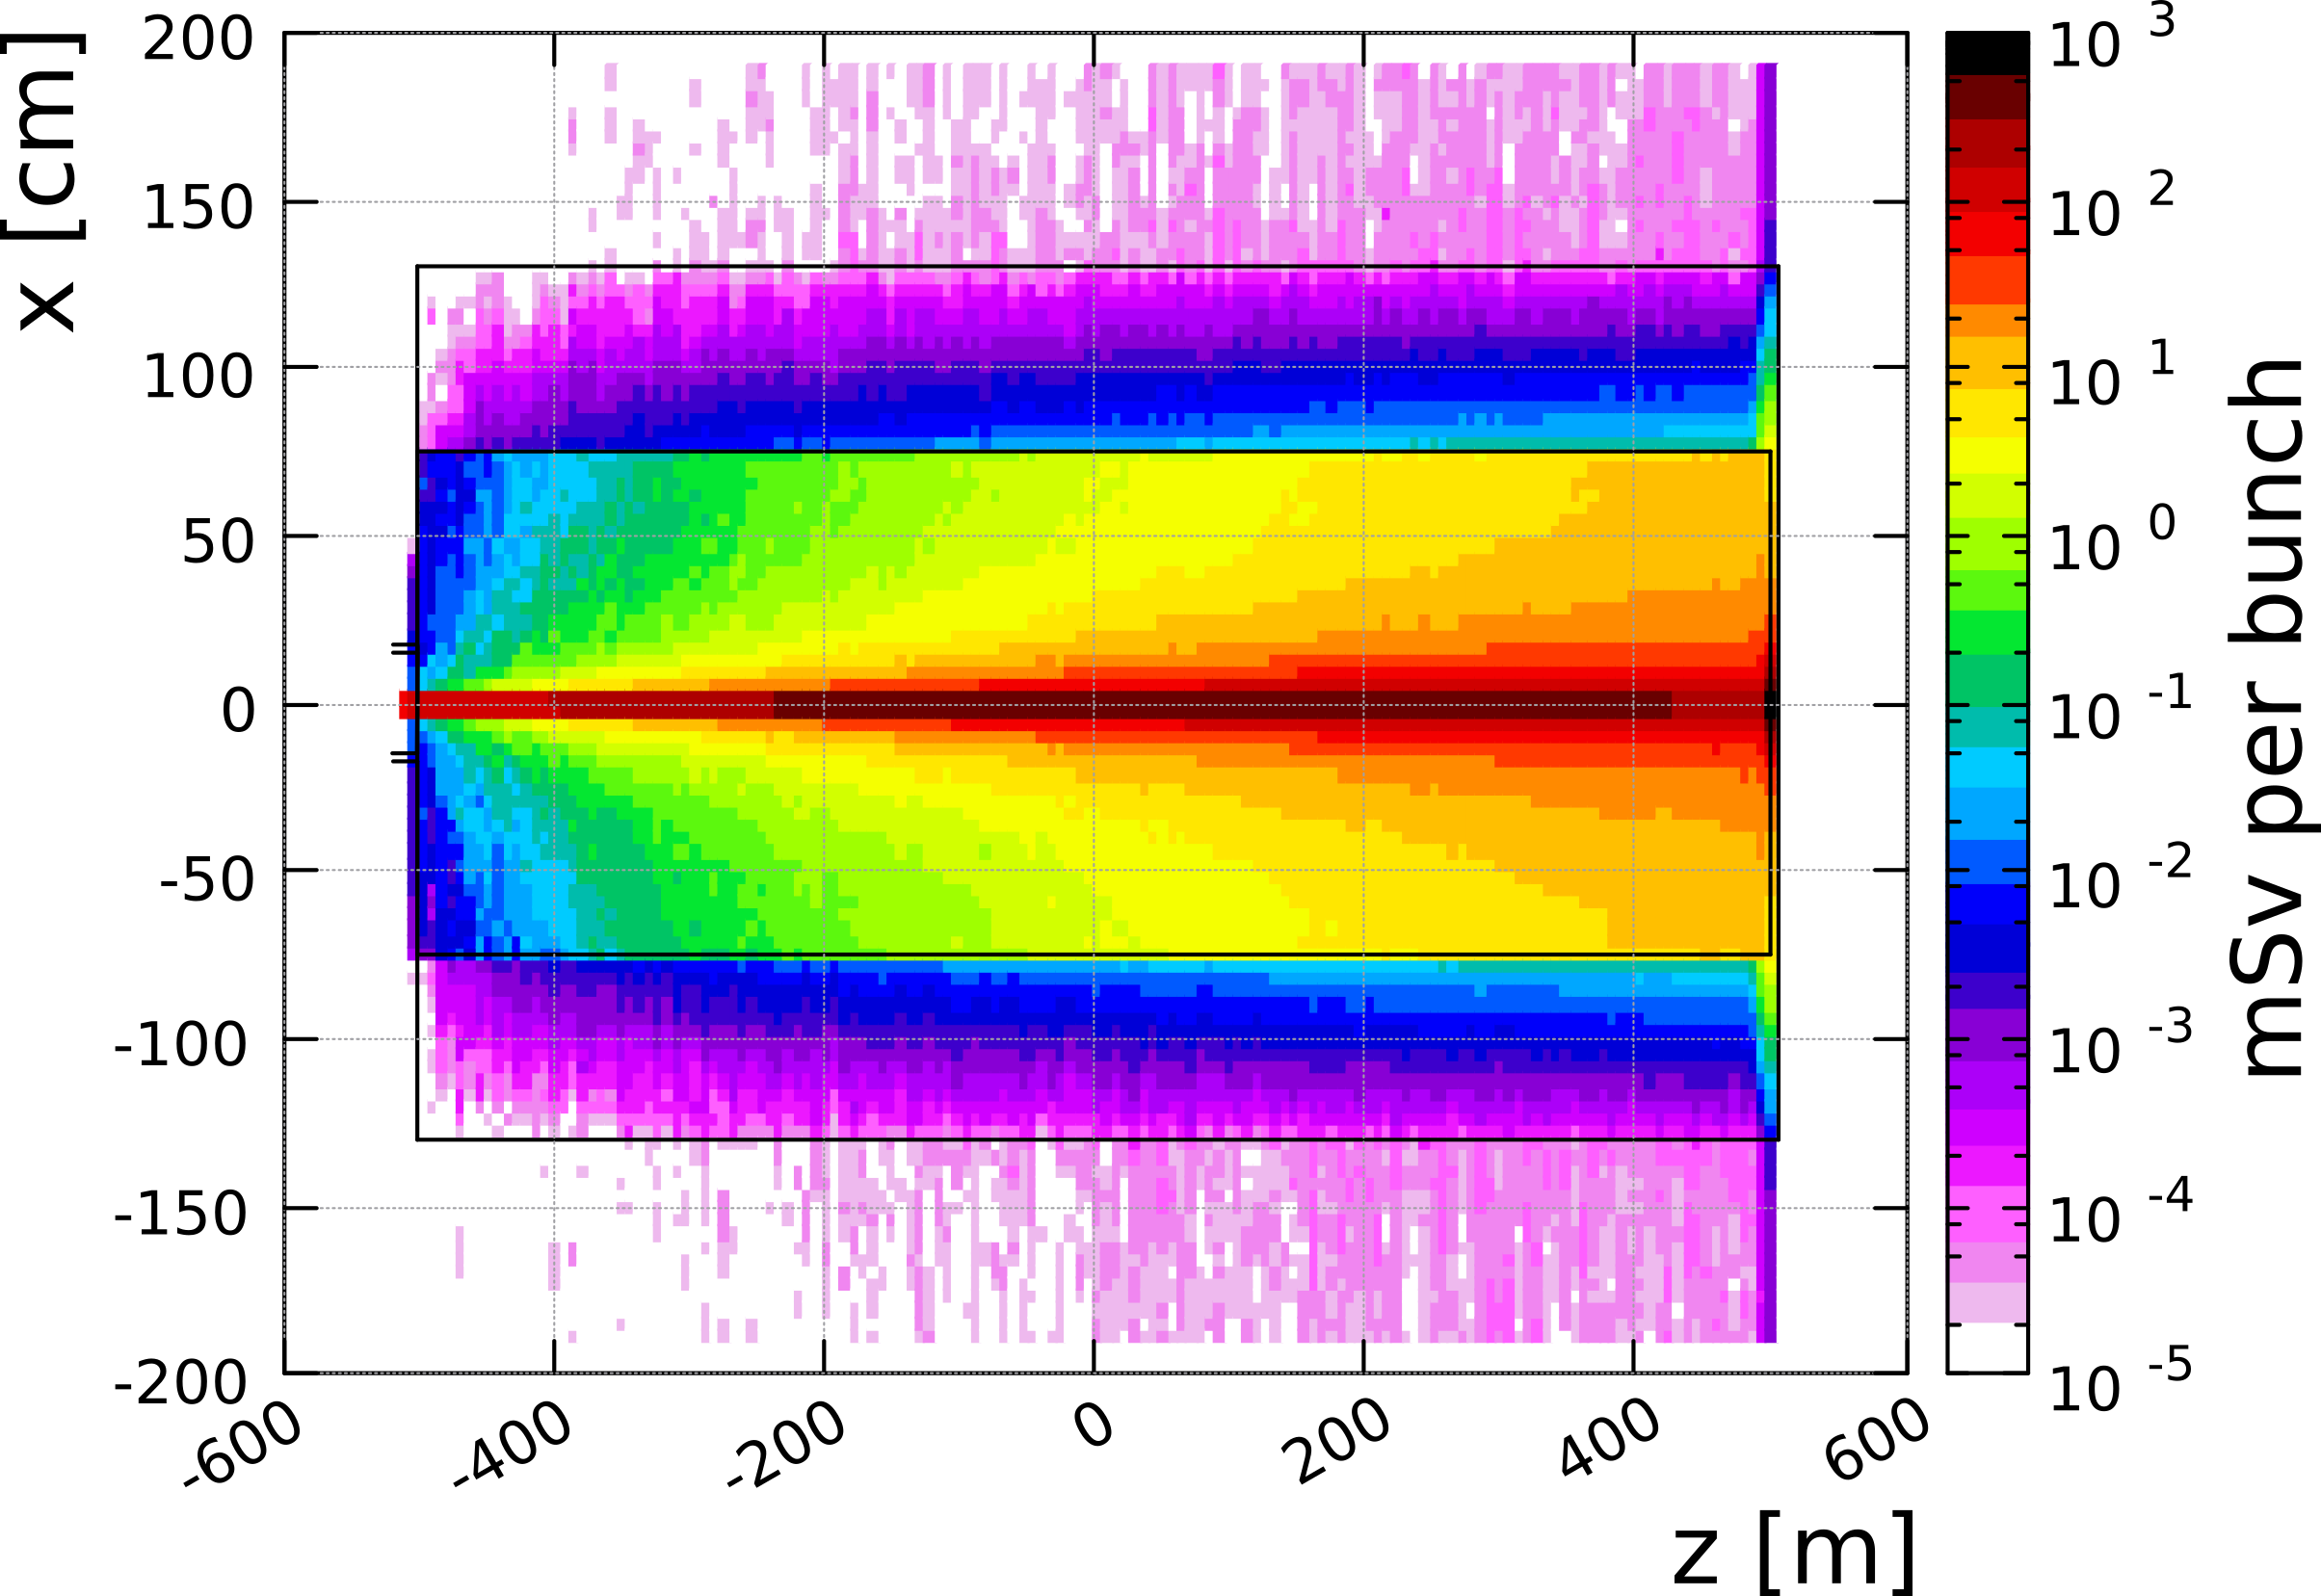
\includegraphics[width=\textwidth]{Figures/BeamDump/Gasdump/Dose_eq.png}
   \caption{Instantaneous dose equivalent}
   \end{subfigure}\\
    \begin{subfigure}[b]{0.49\textwidth}
   \centering
    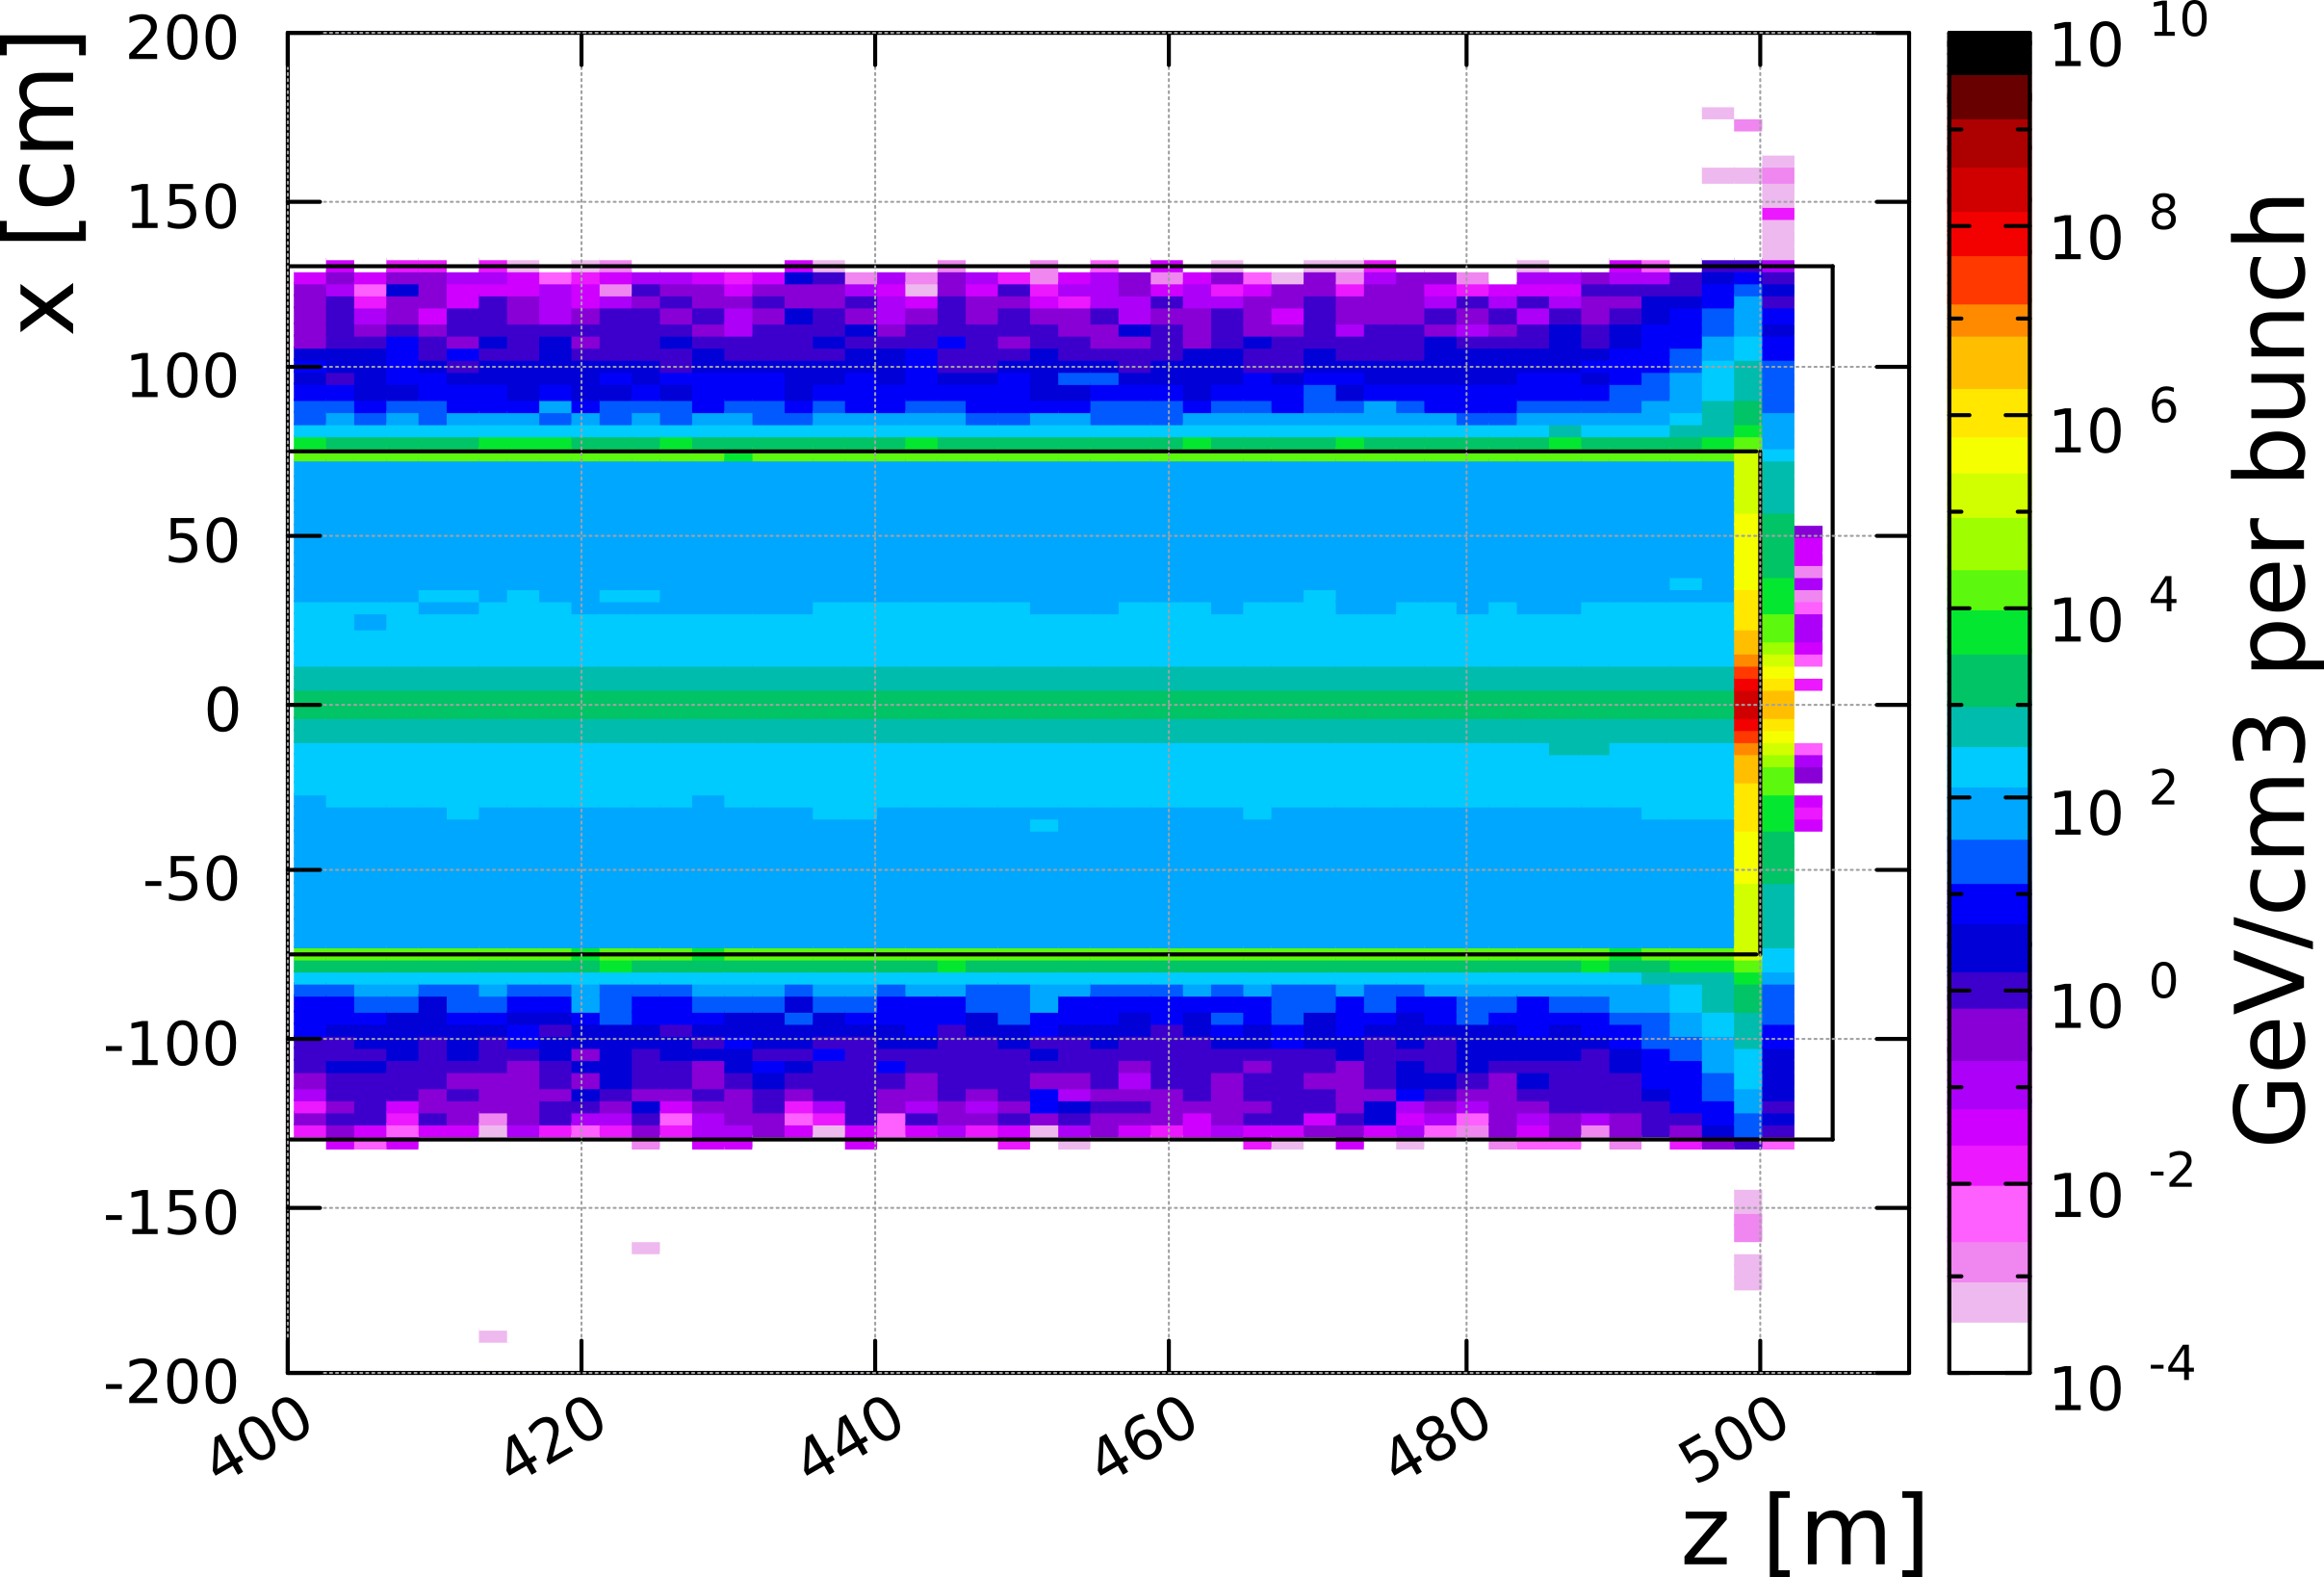
\includegraphics[width=\textwidth]{Figures/BeamDump/Gasdump/Energy_zoom.png}
   \caption{Deposited energy, zoom on vessel end}
   \end{subfigure}
   \hfill
   \begin{subfigure}[b]{0.49\textwidth}
   \centering
    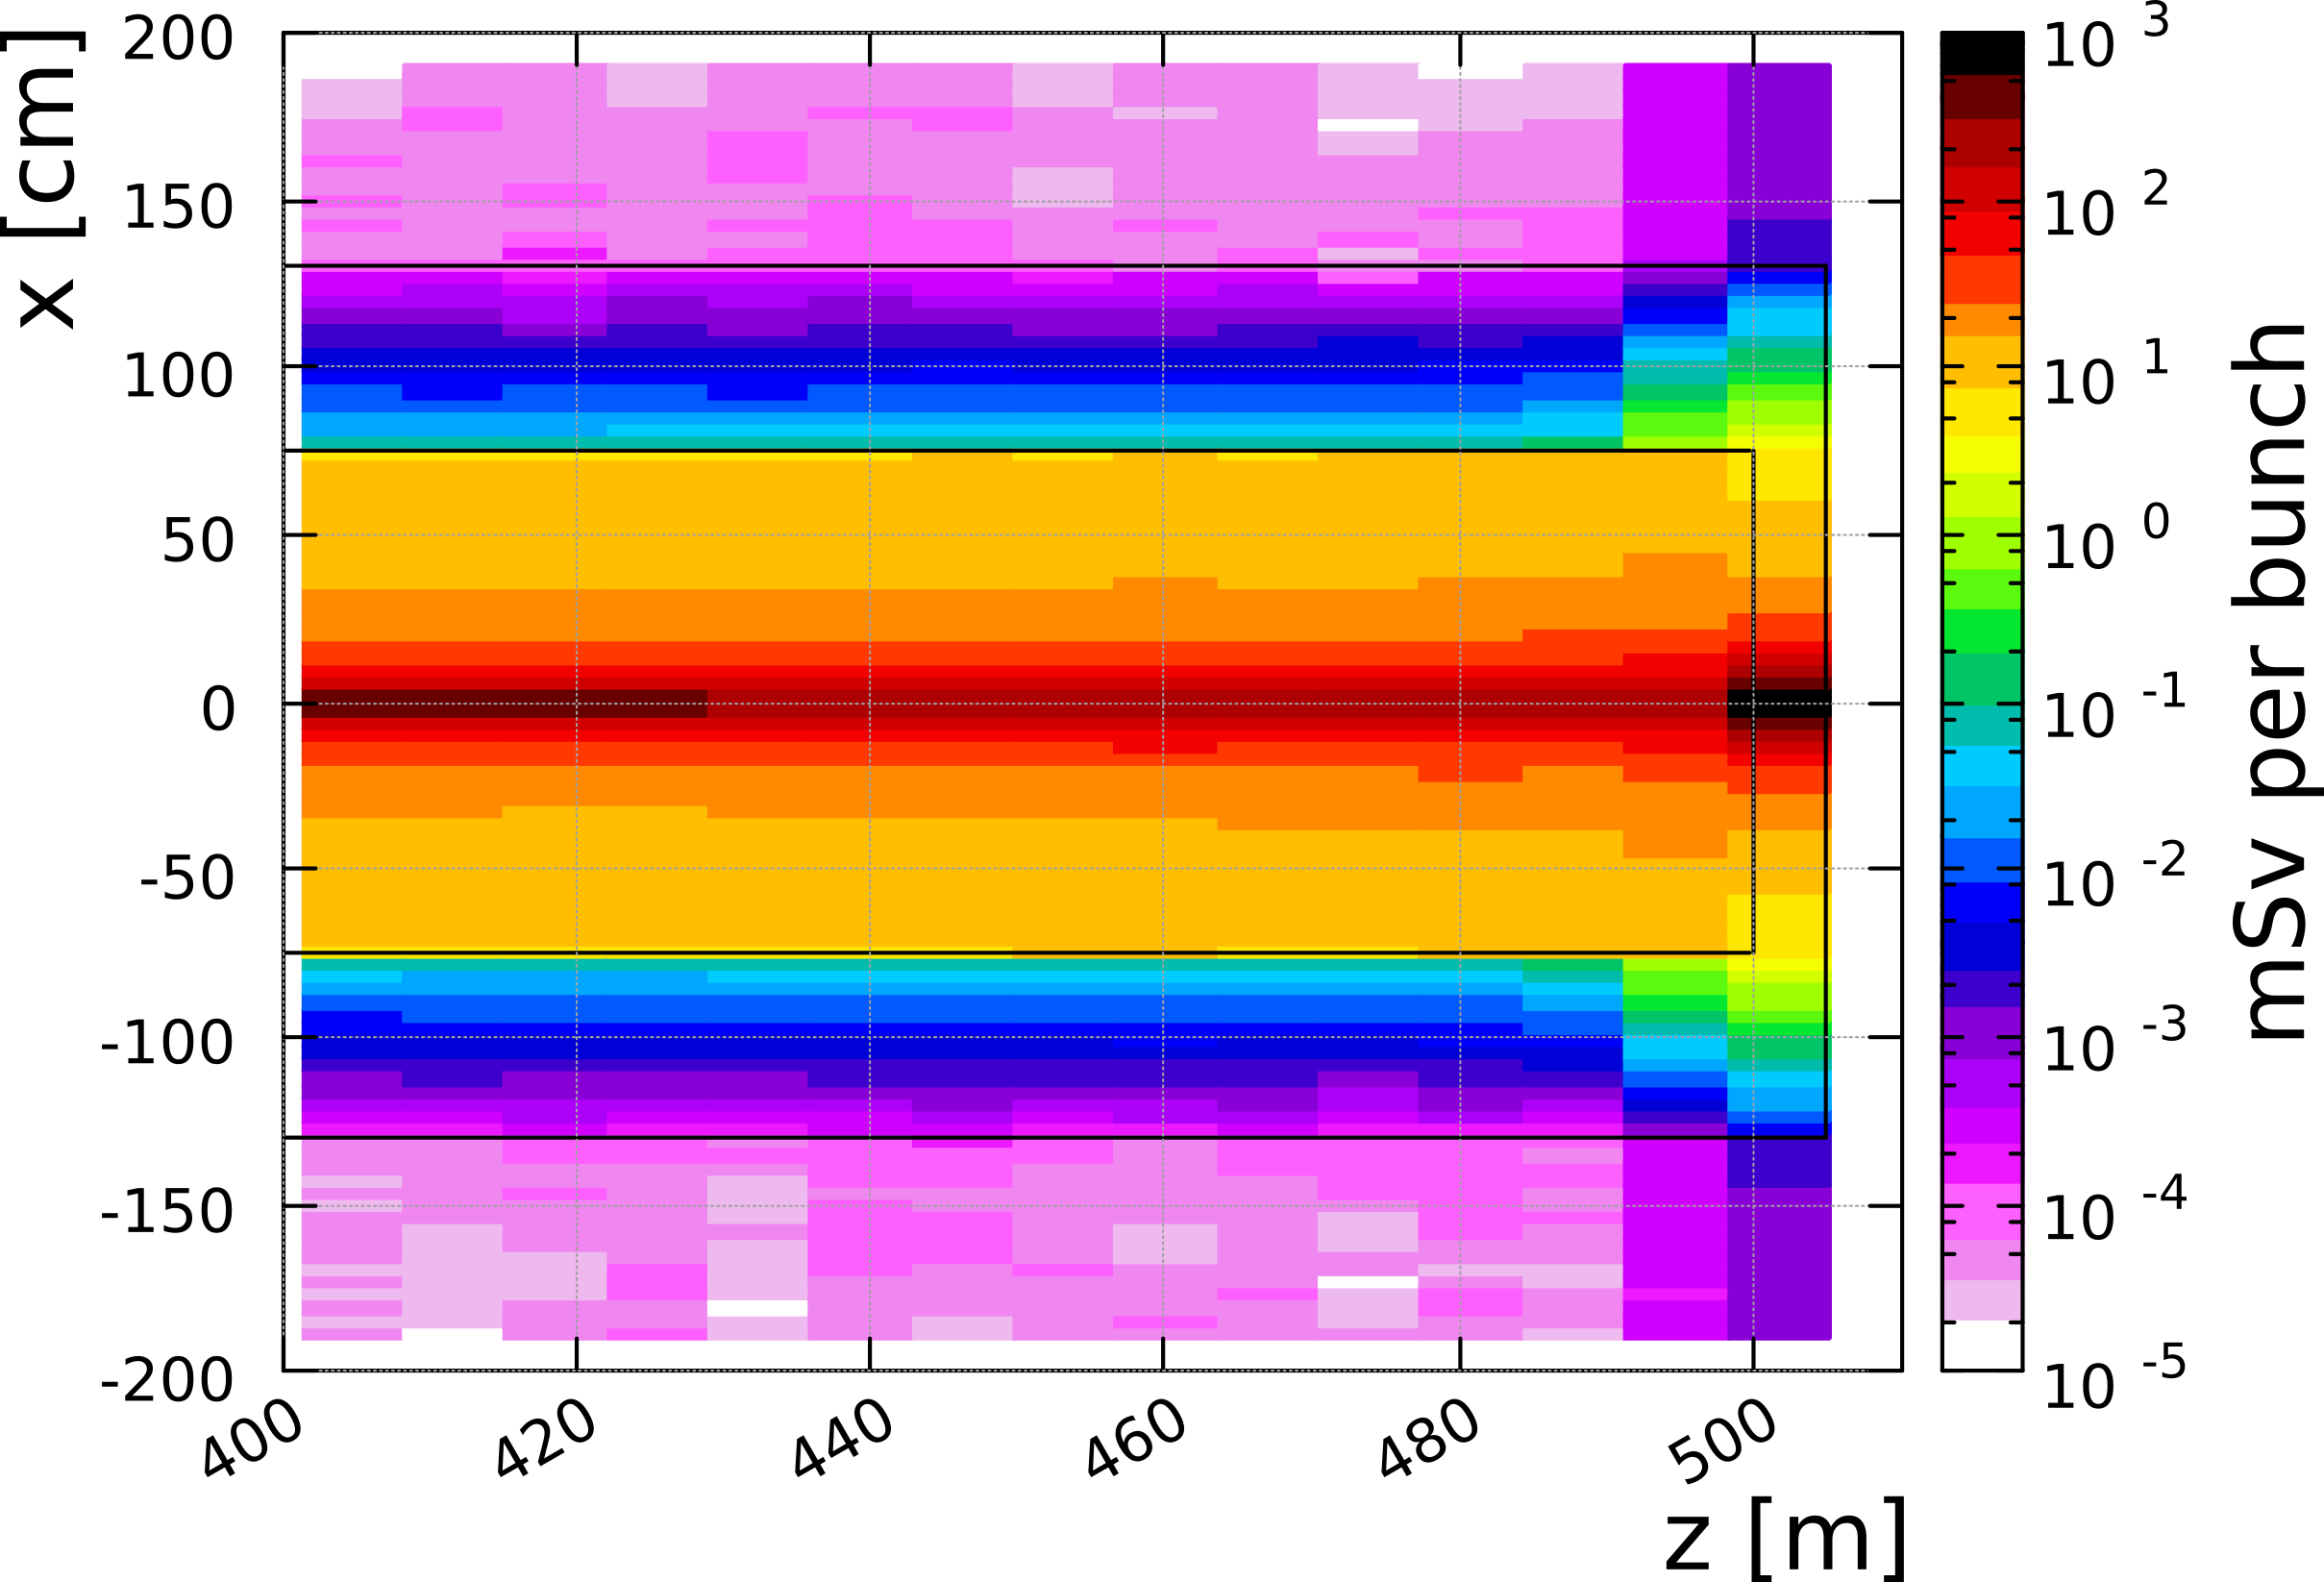
\includegraphics[width=\textwidth]{Figures/BeamDump/Gasdump/Dose_eq_zoom.png}
   \caption{Instantaneous dose equivalent, zoom on vessel end}
   \end{subfigure}
   \caption[Deposited energy and dose equivalent in a gaseous beam dump]{
   \fluka simulation results of a gaseous beam dump vessel.
   \\Figures (a) and (c) show the deposited energy per ILC bunch in the xz-plane.
   The color scale indicates the energy in \si[detect-all]{\GeV}/\si{\centi\meter\cubed}.
   \\Figures (b) and (d) show the resulting dose equivalent in the xz-plane.
   The color scale indicates the dose equivalent in \si[detect-all]{\milli\sievert}/\si{\centi\meter\cubed}.}
   \label{fig:BeamDumps:GasDump}
\end{figure} 

\subsection{Neutron flux}
In addition, a scoring plane has been added to the \fluka model of the gaseous beam dump in a similar way and position as in Section~\ref{BeamDumps:sim_surrounding:Particle}.
The aim was to score neutrons, which are created in the vessel and are oriented in the direction of the extraction line.
\\In this gas vessel design, however, there is no observable flux of neutrons that travel back towards the interaction region.

\section{Conclusion and outlook}
This chapter has presented several studies concerning the ILC main beam dumps.
The two studied designs that were described in Section~\ref{BeamDumps:designs} are based on a \SI{12}{\meter} long water vessel.
Both vessel designs, which had been developed for the currently foreseen ILC main beam dumps, contain sophisticated vortex flow systems for dissipating the deposited energy of the beam bunches.
Additional copper plates in the end of the vessels present enough radiation lengths to fully absorb the beam.
The high material densities, however, have been identified with the presented \fluka simulations of the dump designs (Section~\ref{BeamDumps:sim_surrounding}) to lead to high levels of deposited energy inside and outside of the beam dump.
In the water but also in the vessel and shielding materials, radioactive nuclei are produced, which activate the water and the surroundings.
Activation studies in Section~\ref{BeamDumps:sim_surrounding:Dose} have shown that the resulting dose rates after one year of cooling time still reach up to \SI{10}{\milli\sievert\per\second} in the surroundings of the dumps, which represents a large risk for maintenance personnel and demands a restriction of their duration of stay.

Furthermore, particle fluxes have been studied in Section~\ref{BeamDumps:sim_surrounding:Particle}, especially the neutron flux that originates in the water vessel and reaches back towards the extraction line.
Section~\ref{BeamDumps:sim_EXT} presented a second \fluka simulation of the neutrons traveling through the extraction line towards the interaction region, which yielded the four-vectors of the \num{5.9e6} neutrons arriving at the \sid detector.
\\In a full \geant detector simulation, the hits of the neutrons in the \sid subdetectors have been counted, and the arising occupancy has been shown (Section~\ref{BeamDumps:SiDocc}).
Due to the neutron momenta and their spatial distribution, the hits are contained within the outermost layers of the \sid muon system and the BeamCal.

The results of the activation study but also of the neutron background study suggest to consider a different approach for the ILC main beam dumps.
In an additional \fluka simulation explained in Section~\ref{BeamDumps:Alternative}, a model of a gaseous beam dump has been studied with respect to the deposited energy, the dose equivalent, and the arising neutron flux.
In all three matters, the gaseous beam dump design yields results that are several orders of magnitude better than the water dump designs.
The beam energy is dissipated throughout the length of the gas dump, and is then fully absorbed at the end of the \SI{1}{\kilo\meter} long vessel.
This leads to a spatial restriction of the irradiation to the gas volume and the vessel back wall.
In addition, no measurable neutron flux at the entrance to the beam dump hall was observed in the \fluka simulation.

Overall, a gaseous dump seems to be more suitable with respect to the irradiation and the radiation safety.
Due to the required length of the vessel, in order to fully dissipate and absorb the beam power, the cost for the necessary tunnel is a clear disadvantage of this approach.
For calculating the construction cost of the ILC main linac tunnel, an estimation of \num{22000}\,\euro\,per one meter of tunnel length has been used~\cite{TunnelCost}.
Using this estimation, the cost for the two required gaseous beam dump tunnels (each is \SI{1}{\kilo\meter} long) would be in total \num{44}\,million\.\euro.
Due to the ILC cost constraints, a gaseous beam dump has not been considered as an option for the ILC.
The clear advantages, however, are not to be neglected.
Even if the gaseous beam dumps are a large cost addition, they would save the expenses of costly radiation safety measures for the water dump surroundings, such as the remote handling systems which have been mentioned above.